% University of Michigan Dissertation LaTeX Template for 2019 -- 2020
% Created by John Meluso and Shreyas Kousik
% 9 Jul 2020

% Use the University of Michigan thesis class.
\documentclass[thesis]{thesis-umich}
%%% Packages included in thesis-umich class
%\RequirePackage[margin=1in,footskip=8pt,headsep=0.4cm,headheight=\baselineskip]{geometry}
%\RequirePackage{amsmath}
%\RequirePackage{amsfonts}
%\RequirePackage{amssymb}
%\RequirePackage{graphicx}
%\RequirePackage{subcaption}
%\RequirePackage{times}
%\RequirePackage{natbib}
%\RequirePackage{verbatim}
%\RequirePackage{upquote}
%\RequirePackage{textcomp}
%\RequirePackage{setspace}
%\RequirePackage{ifthen}
%\RequirePackage{soul}
%\RequirePackage{float}
%\RequirePackage[printonlyused]{acronym}
%\RequirePackage{makeidx}
%\RequirePackage{fancyhdr}
%\RequirePackage{multicol}

\usepackage{blindtext} % Example package which populates the ever-popular lorem ipsum text.

%
\usepackage{siunitx, textgreek, chemformula}
\sisetup{group-digits=integer,group-separator={,}}

% cleveref
\usepackage{cleveref}
\renewcommand{\thesubfigure}{\Alph{subfigure}}
\newcommand{\myref}[1]{\Cref{#1}}
\newcommand{\mysubref}[1]{\subref{#1}}
\newcommand{\phantomsubfiglabel}[1]{
    \begin{subfigure}[t]{0\textwidth} % hidden, reference-only
         \phantomcaption
         \label{#1}   
    \end{subfigure}
}


% use French spacing
\frenchspacing

% \justifying
\usepackage{ragged2e}

\usepackage{seqsplit}
\newcommand{\gene}[1]{\textit{\uppercase{#1}}}
\newcommand{\GE}[1]{\textit{#1}}% other genetic elements
\newcommand{\bacterialgene}[1]{\textit{#1}}
\newcommand{\protein}[1]{\uppercase{#1}}
\newcommand{\Latin}[1]{\textit{#1}}
\newcommand{\Oligo}[1]{\texttt{5'-\uppercase{\seqsplit{#1}}-3'}}
\newcommand{\MixedOligo}[1]{\texttt{5'-\seqsplit{#1}-3'}}
\newcommand{\Peptide}[1]{\texttt{\seqsplit{#1}}}



% need cite/citation/reference?

% If you are using the alpha bibliography style, keep these next three lines in your preamble, so that the references are left-aligned; or, you can comment it out and see what happens
\makeatletter
\renewcommand{\@biblabel}[1]{[#1]\hfill}
\makeatother

% Title of the thesis
\title{Quantitative and mechanistic studies on the spindle assembly checkpoint in human cells imply the origin of its sensitivity}

% Author name
\author{Chu Chen}

% Department
\department{Biophysics}

% Year of completion
\year=2022

% Author email
\email{chenchu@umich.edu}

% Author ORCID iD
\orcid{0000-0002-5075-5722}

% Frontispiece
%\frontispiece{\includegraphics[width=4in]{front_materials/frontispiece.png}}

% Default style for front pages
\frontpagestyle{7} % 7 is preferred by Rackham, but should be set individually for each front page

% Dedication (the input [7] determines the style -- 7 is Rackham's preferred style)
% \hidededication{%
\dedication[7]{I would like to dedicate this work to my grandparents. I was not able to stay by their side during their last days because I have been studying far away from my hometown since 2011. They were always caring about me and had a tremendous impact on me and the path that I chose. May them rest in peace.}

% Acknowledgments (the input [7] determines the style -- 7 is Rackham's preferred style)
\acknowledgments[7]{I would like to express my deepest gratitude to my advisor, Dr. Ajit Joglekar. Pursuing a Ph.D. degree is arduous, especially for me as an international student during a challenging time. Ajit has always been supporting me in many aspects.

I am grateful to all members of my thesis committee, who have kindly offered their time and expertise to give me guidance, suggestions, and comments on my research for nearly six years.

I would like to acknowledge all of my lab colleagues (Dr. Arti Dumbrepatil, Martin Fernandez, Frank Ferrari, Adrienne Fontan, Simon Han, Lauren Humphrey-Stark, Soubhagyalaxmi Jema, Shriya Karmarkar, Sisira Kavuri, Dr. Alex Kukreja, Andrew Livingston, Sean McGuire, Anna Olson, Juan Orozco, Rebekah Ronan, Dr. Babhrubahan Roy, Janice Sim, Dr. Vikash Verma, and Alex Vita) who have supported my work in the lab by directly participating in my research (which is credited in corresponding parts of the main text of this thesis), offering valuable suggestions, and building up a healthy work environment.

Our collaborators have taught me a lot about science and have greatly enhanced the breadth and impact of our research. They include (but are not limited to): Dr. Iain Cheeseman (Whitehead Institute); Dr. John Tyson and Dr. Anand Banerjee (Virginia Tech); Dr. Geert Kops (Hubrecht Institute, Netherlands); Dr. Song-Tao Liu and Dr. Yibo Luo (University of Toledo); Dr. Andrea Musacchio and Dr. Valentina Piano (MPI of Molecular Physiology, Germany).

Many other friends and colleagues have helped me greatly in this endeavor, either by directly solving my technical problems or offering key suggestions over the years. They include (but are not limited to): Dr. Mara Duncan (experimental techniques); Dr. J. Damon Hoff (fluorescence spectroscopy and associated data analysis); Dr. Dawei Yang (image processing and pattern recognition); Dr. Uhn-Soo Cho as well as Dr. Sojin An and Dr. Jennifer Chik (molecular cloning and protein purification); Dr. Diane Fingar and Dr. Dubek Kazyken (kinase assay); Dr. Fengrong Wang and Dr. Takamasa Inoue (immunoprecipitation); Dr. Chengxin Zhang (structure prediction); Dr. Xiangtian Tan (bioinformatics); Dr. Nigel Michki and Dr. Kyoung Jo (fluorescence imaging); Dr. Zhejian Ji (spindle assembly checkpoint). Many others provided me with necessary reagents and instruments, whose assistance was or will be acknowledged in my published paper \cite{eSAC} and other manuscripts in preparation or under review.

I would like to thank my mentors during my first-year rotations (Dr. Tom Kerppola and Dr. Wei Cheng). Although I did not join their labs, I am thankful for their close guidance at the early stage of my academic pursuit.%Also, I have broadened my view through exchanges with many members from Dr. Ryoma Ohi's lab and Dr. Uhn-Soo Cho's lab.

Last but not least, I could not have reached so far without the support and inspiration from my family and friends. They are my pole star and lighthouses in this memorable voyage.}

% Preface
% \preface[7]{\input{front_materials/preface}}

% Committee
\committee{
Associate Professor Ajit P. Joglekar, Chair \\
Professor Julie S. Biteen \\
Assistant Professor Aaron T. Frank \\
Professor David K. Lubensky \\
Professor Yukiko Yamashita, Whitehead Institute \\
Assistant Professor Qiong Yang \\
}

% Chair must be entered separately for formatting reasons.
\chair{Professor First Name}
%\cochair{Co-chair One \& Co-chair Two}

% Commands to hide or show lists of figures, tables, etc.
\showlistoftables
%\showlistofprograms
%\showlistofappendices


% Definition of any acronyms used.
\acronyms{
\acro{a.a.}{amino acid(s) (number)}
\acro{ABBA motif}{A-type cyclins, BUBR1, BUB1, and Acm1 consensus motif}
\acro{DMEM}{Dulbecco's modified Eagle's medium}
\acro{FCS}{fluorescence correlation spectroscopy}
\acro{FRB*}{FRB with a T2098L point mutation}
\acro{FRET}{F{\"{o}}rster resonance energy transfer}
\acro{HD}{heterodimerization domain (a.a. 432-484) of \protein{BubR1}}
\acro{HD$^{short}$}{heterodimerization domain (a.a. 440-460) of \protein{BubR1}}
\acro{KARD}{kinetochore attachment regulatory domain of \protein{BubR1}}
\acro{LUT}{lookup table}
\acro{MCC}{mitotic checkpoint complex (consisting of \protein{Cdc20}, \protein{Mad2}, \protein{BubR1}, and \protein{Bub3})}
\acro{MELT$^n$}{the $n$-th MELT motif among the 19 putative MELT motifs in human \protein{Knl1}}
\acro{MIM}{MAD2-interacting motif (also named as MAD2-binding motif or MBM in previous literature)}
\acro{mNG}{mNeonGreen}
\acro{NEBD}{nuclear envelope breakdown}
\acro{NPC}{nuclear pore complex}
\acro{RACE}{rapid amplification of cDNA ends}
\acro{RMCE}{recombination-mediated cassette exchange}
\acro{RT}{reverse transcription}
\acro{RWD domain}{RING finger-containing proteins, WD repeat-containing proteins, and DEAD-like helicases domain}
\acro{RZZS}{ROD-Zwilch-ZW10-Spindly}
\acro{SAC}{spindle assembly checkpoint}
\acro{SEM}{standard error of the mean}
\acro{TRE}{tetracycline-responsive promoter element}
\acro{TSS}{transcription start site}
\acro{UTR}{untranslated region}
\acro{WT}{wildtype}
}

% Some abstract text
\abstract{
Equal distribution of replicated genetic materials packed in chromosomes from a dividing parent cell to two daughter cells is the hallmark of mitosis. This task is carried out by the spindle, whose microtubules attach to chromosomes through adaptors named kinetochores. Failure to achieve faithful chromosome segregation is often associated with cancers and many pathological syndromes.

My thesis investigates a surveillance mechanism named the spindle assembly checkpoint (SAC) that safeguards faithful chromosome segregation. The SAC is activated at kinetochores lacking end-on spindle microtubule attachment to stall the progression of mitosis. The SAC can robustly arrest a mammalian cell in mitosis in the presence of either many unattached kinetochores or merely one. Although the biochemical events associated with the SAC have been mostly elucidated, how the SAC reaches such ``sensitivity'' to effectively arrest a cell in mitosis in the presence of a single unattached kinetochore remains unclear. Here, I will describe how multiple proteins and reactions cooperate at various layers to enable this sensitivity.

First, to study the origin of the sensitivity of the SAC, we need a quantitative readout of the input (the phosphorylation of the scaffold protein KNL1 which recruits SAC proteins and activates the SAC at signaling kinetochores) and the output (the duration of the mitotic arrest caused by the SAC). In Chapter 2, we engineer a cytosolic probe that ectopically activates the SAC, which solves the technical challenge to gauge the phosphorylation of KNL1 in live cells. Dose-response analyses using the probe reveal that under certain conditions, the SAC signaling activity is stronger with a smaller number of phosphorylated KNL1 proteins. This striking observation strongly indicates positive cooperativity in the SAC, which may underlie the sensitivity of the SAC.

Next, I validate some of the preconditions of this cooperativity model above in the context of the endogenous kinetochore-based SAC in Chapter 3. We demonstrate %that the cytosolic pools of SAC proteins were diminished due to their recruitment to signaling kinetochores and
that the numbers of SAC proteins recruited per signaling kinetochore are inversely correlated with the total number of signaling kinetochores in the cell. Additionally, I show that the localization at signaling kinetochores of BUBR1, an important constituent of the mitotic checkpoint complex (MCC, the effector molecule that stalls the progression of mitosis made up of BUBR1, BUB3, CDC20, and MAD2), strengthens the SAC activity. These observations reinforce the idea that cooperative signaling contributes to the sensitivity of the SAC.

Finally, in Chapter 4, I explore the catalytic mechanism of the rate-limiting step in the assembly of the MCC -- the formation of CDC20-MAD2. Unveiling this catalytic mechanism is fundamental to understanding how an unattached kinetochore can produce an adequate signal to stall mitosis. Given that both CDC20 and MAD2 bind to the catalyst MAD1, I hypothesize that the structural flexibility of MAD1 helps to position CDC20 and MAD2 closely, thereby coordinating the formation of CDC20-MAD2. Our data show that disrupting the structural flexibility of MAD1 impairs the SAC signaling activity, based on which I propose a model for the catalytic mechanism of the formation of CDC20-MAD2 scaffolded by MAD1.

My thesis research reveals the role of cooperative synergy in shaping the sensitivity of the SAC. It also establishes the foundation for future studies aiming for a complete understanding of the origin of its sensitivity.
}
%\hideabstractpagenumber

%% DOCUMENT AREA
\begin{document}

\chapter{Introduction}
\label{chpt:introduction}

%  How the SAC blocks the progression of mitosis in the presence of a single unattached kinetochore and releases the block promptly once all attachment is secured remains unclear. Here, I summarize our discovery that the SAC, like many other biochemical switches, exploits cooperativity to achieve such sensitivity. Furthermore, I look into potential molecular mechanisms of this cooperativity.

% Unattached kinetochores catalyze MCC formation by recruiting SAC proteins in a well-defined signaling cascade (Fig. 1A) (Faesen et al., 2017; Ji et al., 2017; Lara-Gonzalez et al., 2021a; London and Biggins, 2014; London et al., 2012; Piano et al., 2021; Primorac et al., 2013; Shepperd et al., 2012). This cascade is activated when the kinetochore protein Knl1 is phosphorylated by the Mps1 kinase at the ‘MELT’ motifs, so called because of their consensus amino acid sequence in humans and other eukaryotes (Primorac et al., 2013; Tromer et al., 2015; Vleugel et al., 2013). Each MELT motif serves as the scaffold for recruiting downstream signaling proteins (Chen et al., 2019; Primorac et al., 2013).

% Accurate chromosome segregation during cell division requires that the sister kinetochores on each replicated chromosome are stably attached to microtubules emanating from opposite spindle poles before the cell divides. If one or more kinetochores fail to attach to microtubules, they activate a biochemical signaling cascade known as the spindle assembly checkpoint (SAC). This cascade produces an anaphase-inhibitory signal known as the ‘‘mitotic checkpoint complex’’ (MCC). MCC in- hibits the anaphase promoting complex/cyclosome (APC/C) to prevent the cell from transitioning from prometaphase to anaphase, thus avoiding chromosome mis-segregation [2].

\begin{figure}
    \centering
    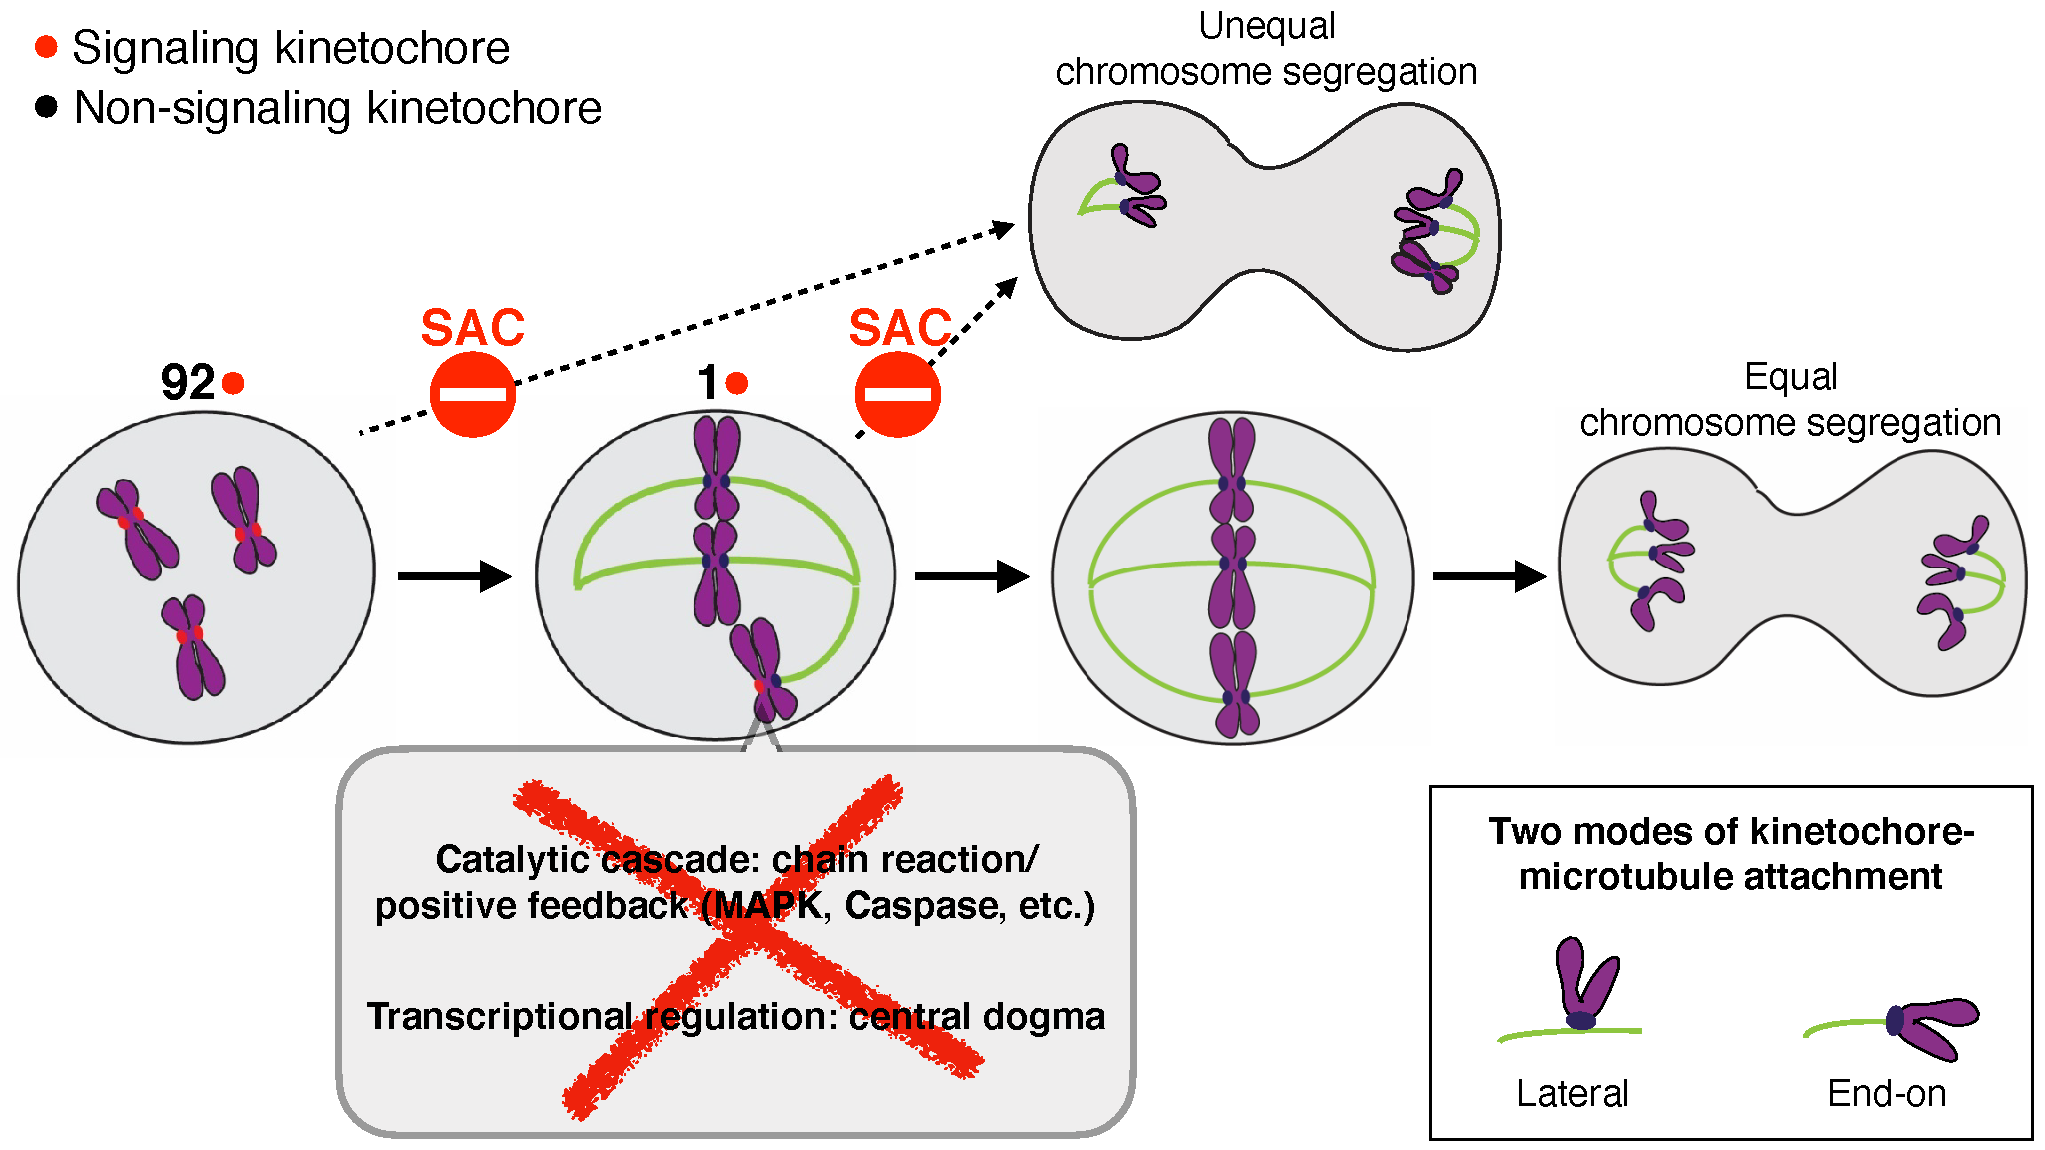
\includegraphics[width=0.9\textwidth]{chapters/figures/SACRole.pdf}
    \caption{\textbf{The role and properties of the SAC.}}
    \noindent\justifying The sensitivity of the SAC is unlikely to be facilitated by an enzymatic amplification cascade, given our current understanding of the biochemical pathway of the SAC \cite{InhibitorUltrasensitivity, Caspase}. Transcriptional regulations that amplify signals via the central dogma and the potential oligomerization of the involved transcriptional factors \cite{TFMultimerization} are also unlikely because the genome is highly condensed in the chromosome during mitosis.
    \label{SACRole}
\end{figure}

\section{MELT motifs and their arrangement in human \protein{Knl1}}

Alternative splicing is common in intrinsically disordered regions mediating protein-protein interactions \cite{DisorderedRegionsAlternativeSplicing}. However, in many mammals, all of Knl1's MELT motifs within a single exon which is one of the longest internal exons in these mammals (\myref{ExonLength}). No alternatively splicing has been recorded for this region. The splicing machinery has to deploy specific mechanisms to splice long exons like this correctly \cite{InternalExon}.

\begin{table}[H]
    \renewcommand{\arraystretch}{1.5}
    \caption{\textbf{The exon encoding all MELT motifs in \protein{Knl1} ranks among the top 0.03\% by length among all curated internal exons in human and mouse.}}
    \noindent\justifying All putative MELT motifs identified in \cite{MELTEvolution} reside within a single exon and all recorded alternative splice variants of \protein{Knl1} contain this exon in listed mammals. Coordinates of exons (of mouse and human) in the CCDS Database \cite{CCDS} were accessed on May 21, 2020. Exons from coding sequences with either a ``Public'' or a ``Reviewed, update pending'' status were pooled. Redundant entries were removed (because various coding sequences may share a common exon) and the ranking of the MELT motif-encompassing exon was calculated. Due to the lack of data for untranslated regions, only internal exons were included in the analysis. It should be noted that the maximum length of an exon is restricted by the length of the respective protein, and \protein{KNL1} is a long protein of \SI{2342}{} amino acids (the canonical isoform). In a non-canonical isoform of human \protein{Knl1}, this MELT motif-encompassing exon is 166 bases shorter, but still includes all 19 putative MELT motifs.
    \label{ExonLength}
    \begin{center}
        \begin{tabular}{c c c}
            \hline
            Species & Exon length (bases) & Ranking among all curated internal exons\\
            \hline
            Human & 5001 & $99.973\%$\\
            Mouse & 4497 & $99.975\%$\\
            Rat & 3439 & N/A\\
            Cattle & 4020 & N/A\\
            Elephant & 4023 & N/A\\ % What kind of elephant?
            Giant panda & 4017 & N/A\\
            Dog & 3837 & N/A\\
            Bonobo & 3927 & N/A\\
            \hline
        \end{tabular}
    \end{center}
\end{table}

\section{The sensitivity and responsiveness of the SAC}

% Just like one will not completely understand how a machine works just by knowing all the gears involved, we cannot claim to have completely comprehended how the SAC works by just knowing all associated biochemical reactions individually.
% the sensitivity of the SAC
% responsiveness (releasing the block promptly once all attachment is secured)
% How the number of signaling kinetochores changes the strength of the signaling output is not fully understood. This knowledge will help us comprehend how the SAC prevents premature anaphase onset in the presence of a decreasing number of signaling kinetochores from the nuclear envelope breakdown to the metaphase during normal mitotic progression.

\section{Cooperativity and ultrasensitivity}

Originally, ``cooperativity'' was used to described the binding of oxygen molecules to the multi-subunit hemoglobin \cite{KNF, MWC}. Cooperativity may amplify the signal or at least sensitize the output by reducing the dampening effect of any changes in the input \cite{CooperativityQA}. To explain such dampening effect, suppose that the output $f(x) \geq 0$ is a monotonically increasing and strictly concave function of the input $x$ for all $x \geq 0$ (like the Langmuir adsorption equation or the Michaelis-Menten kinetics) and that the output is 0 if and only if the input is 0. Comparing the outputs [$f(x_2)$ and $f(x_1)$] corresponding to the inputs ($x_2 > x_1 > 0$), we have

\begin{equation*}
    1 < \dfrac{f(x_2)}{f(x_1)} = \dfrac{f(x_2)}{f[\dfrac{x_1}{x_2} \cdot x_2 + (1-\dfrac{x_1}{x_2}) \cdot 0]} < \dfrac{f(x_2)}{\dfrac{x_1}{x_2}f(x_2) + (1-\dfrac{x_1}{x_2})f(0)} = \dfrac{x_2}{x_1},
\end{equation*}

\noindent which states that the contrast between the outputs is less than the contrast between the inputs \cite{InhibitorUltrasensitivity}. Due to the wide applicability of the Langmuir adsorption equation or the Michaelis-Menten kinetics in biochemical interactions or reactions, the dampening effect may actually be very common.

There are many well-studied mechanisms (including cooperativity) deployed by signaling cascades exhibiting a switch-like sigmoidal dose-response relationship (ultrasensitivity) to circumvent the dampening effect. Regarding the SAC signaling, certain mechanisms (like the cascade amplification mechanism; see \myref{SACRole}) may be excluded based on our current understanding of mitosis and the biochemical pathway of the SAC, while the multi-step/multi-site phosphorylation mechanism has been implied in the SAC by experimental evidence \cite{MultistepUltrasensitivity, Ji2017eLife} (see the magenta arrows and texts in \myref{CoreSAC}). My thesis will focus on the implied role of cooperativity in the SAC signaling. The term ``positive cooperativity'' (henceforth simply referred to as ``cooperativity'') describes the phenomenological synergy which I attribute to increased local concentration of SAC proteins due to their co-localization on the same signaling scaffold (see my models in \myref{ProzoneEffectModel,FinalKnittingModel}. This is reminiscent of the theoretical explanation of the avidity between antibodies and antigens \cite{AvidityMath}, another well-characterized example of cooperativity.

\section{Methods of studying the SAC quantitatively \Latin{in vivo} and technical challenges}
% The understanding of the entire picture is hindered by multiple difficulties. First, the biochemical reactions that lead to MCC formation are spatially localized within the nanoscale volume of a kinetochore. Second, the concentrations of many SAC proteins are tightly regulated and may be influenced by each other. Third, that the biochemical cascade involves complex parallel recruitment pathways of certain SAC proteins and regulating kinases/phosphatases. 

%To study the quantitative relationship between the strength of the SAC signaling and the number of signaling kinetochores/the amount of SAC proteins localized to signaling kinetochores, The SAC was then activated by treating the cells with either GSK923295 or a high dosage of nocodazole. GSK923295 inhibits the ATPase activity of \protein{Cenp-E}, thereby disrupting chromosome congression and yielding small numbers of chromosomes near spindle poles in mammalian cells \cite{GSK923295}.
% when applied at 75 nM -- 236 nM used in this study
%These polar chromosomes typically possess one kinetochore that is unattached or laterally attached to spindle microtubules, both of which activate the SAC in mammalian cells \cite{GSK923295MonastrolCotreatment,GSK923295LateralAttachmentEM,LateralAttachmentSAC}.
% Monastrol co-treatment may have created the bias towards unattachment instead of lateral attachment.
%Nocodazole affects the dynamics of microtubules and distorts spindles at \SI{330}{nM} in human cells \cite{TypeIIISpindle_330nMNoc, RPE1+Noc}, turning on SAC signaling at almost all kinetochores based on the recruitment of SAC proteins (see below). We applied various fluorescence microscopy and spectroscopy techniques to quantify SAC proteins and their influence on the SAC in live cells \cite{eSAC}. % Small numbers of signaling kinetochores and relative enrichment of SAC proteins on them.

%This chromosome congression-promoting function complicates the quantitative study of the SAC signaling output in live cells.
\chapter{Ectopic activation of the spindle assembly checkpoint reveals its dose-response characteristics}
\label{chpt2}

Ideally, the SAC should respond to a single unattached (or laterally attached) kinetochore in a dividing cell. Indeed, a single unattached kinetochore delays anaphase onset in mitotic PtK1 cells \cite{PtK1SingleUnattachedKT}. However, the SAC may be less stringent in the first few cleavages of mammalian zygotes \cite{MouseEmbryoSAC, ParentalGenomeUnification}. To understand how the SAC responds to the changing number of signaling kinetochores over the progression of mitosis (\myref{SACRole}), it is necessary to quantify its dose-response characteristics. However, it is technically demanding to maintain a specific number of signaling kinetochores in the cells \cite{Ablation}, especially when a large number of cells are required to counter the noise.

This chapter describes a novel ectopic SAC (eSAC) activator, which activates the SAC independently of the status of kinetochore-microtubule attachment in human cells. By exploiting heterogeneous expression of eSAC activators in a large population of cells, we defined the dependence of the eSAC activator-induced mitotic arrest on the abundance of the eSAC activator to reveal the dose-response characteristics of the core SAC signaling cascade. The critical role of cooperativity is implied in modulating how the SAC responds to the changing number of signaling kinetochores to achieve aforementioned sensitivity in the mitosis of somatic cells.

This chapter is paraphrased and adapted from \cite{eSAC}, with the addition of new references and some of my unpublished data. Key experiments and data mentioned in this chapter to which I am not a main contributor are referred back to the published paper and credited accordingly (those figures are not reproduced here). Certain statements in the original discussion have been adjusted to reflect the up-to-date understanding of the SAC. However, the basic ideas and main conclusions stay the same as in the original paper.

\section{Engineering an ectopic SAC (eSAC) activator}
The SAC signaling is initiated by the phosphorylation of MELT motifs in \protein{Knl1} by \protein{Mps1} at unattached (or laterally-attached) kinetochores \cite{MPS1-KNL1_London2012, MPS1-KNL1_Shepperd2012, MPS1-KNL1_Yamagishi2012, GSK923295MonastrolCotreatment, GSK923295LateralAttachmentEM, LateralAttachmentSAC}. It should be possible to bypass the involvement of kinetochores and activate the SAC signaling by bringing \protein{Mps1} into close proximity with \protein{Knl1}. Previous studies have shown that the SAC can be activated ectopically (independently of the status of kinetochore-microtubule attachment) by overexpressing Mps1 in the budding yeast \cite{Mps1pOverexpressionActivatesSAC}, anchoring \protein{Mad1} to metaphase kinetochores in human cells \cite{HeLa-A12_Ballister2014}, or dimerizing Knl1 with Mps1 in the budding yeast \cite{BuddingYeasteSAC} or the fission yeast \cite{FissionYeasteSAC}. Inspired by these results, we engineered an ectopic SAC (eSAC) activator consisting of a recombinant \protein{Knl1} phosphodomain and a recombinant \protein{Mps1} kinase domain (\myref{eSAC}). They are fused with the chemical-induced dimerization system, wherein FKBP and FRB bind to each other in a rapamycin-dependent manner with high specificity and affinity \cite{FKBP-Rapamycin-FRB}.

\begin{figure}
    \centering
    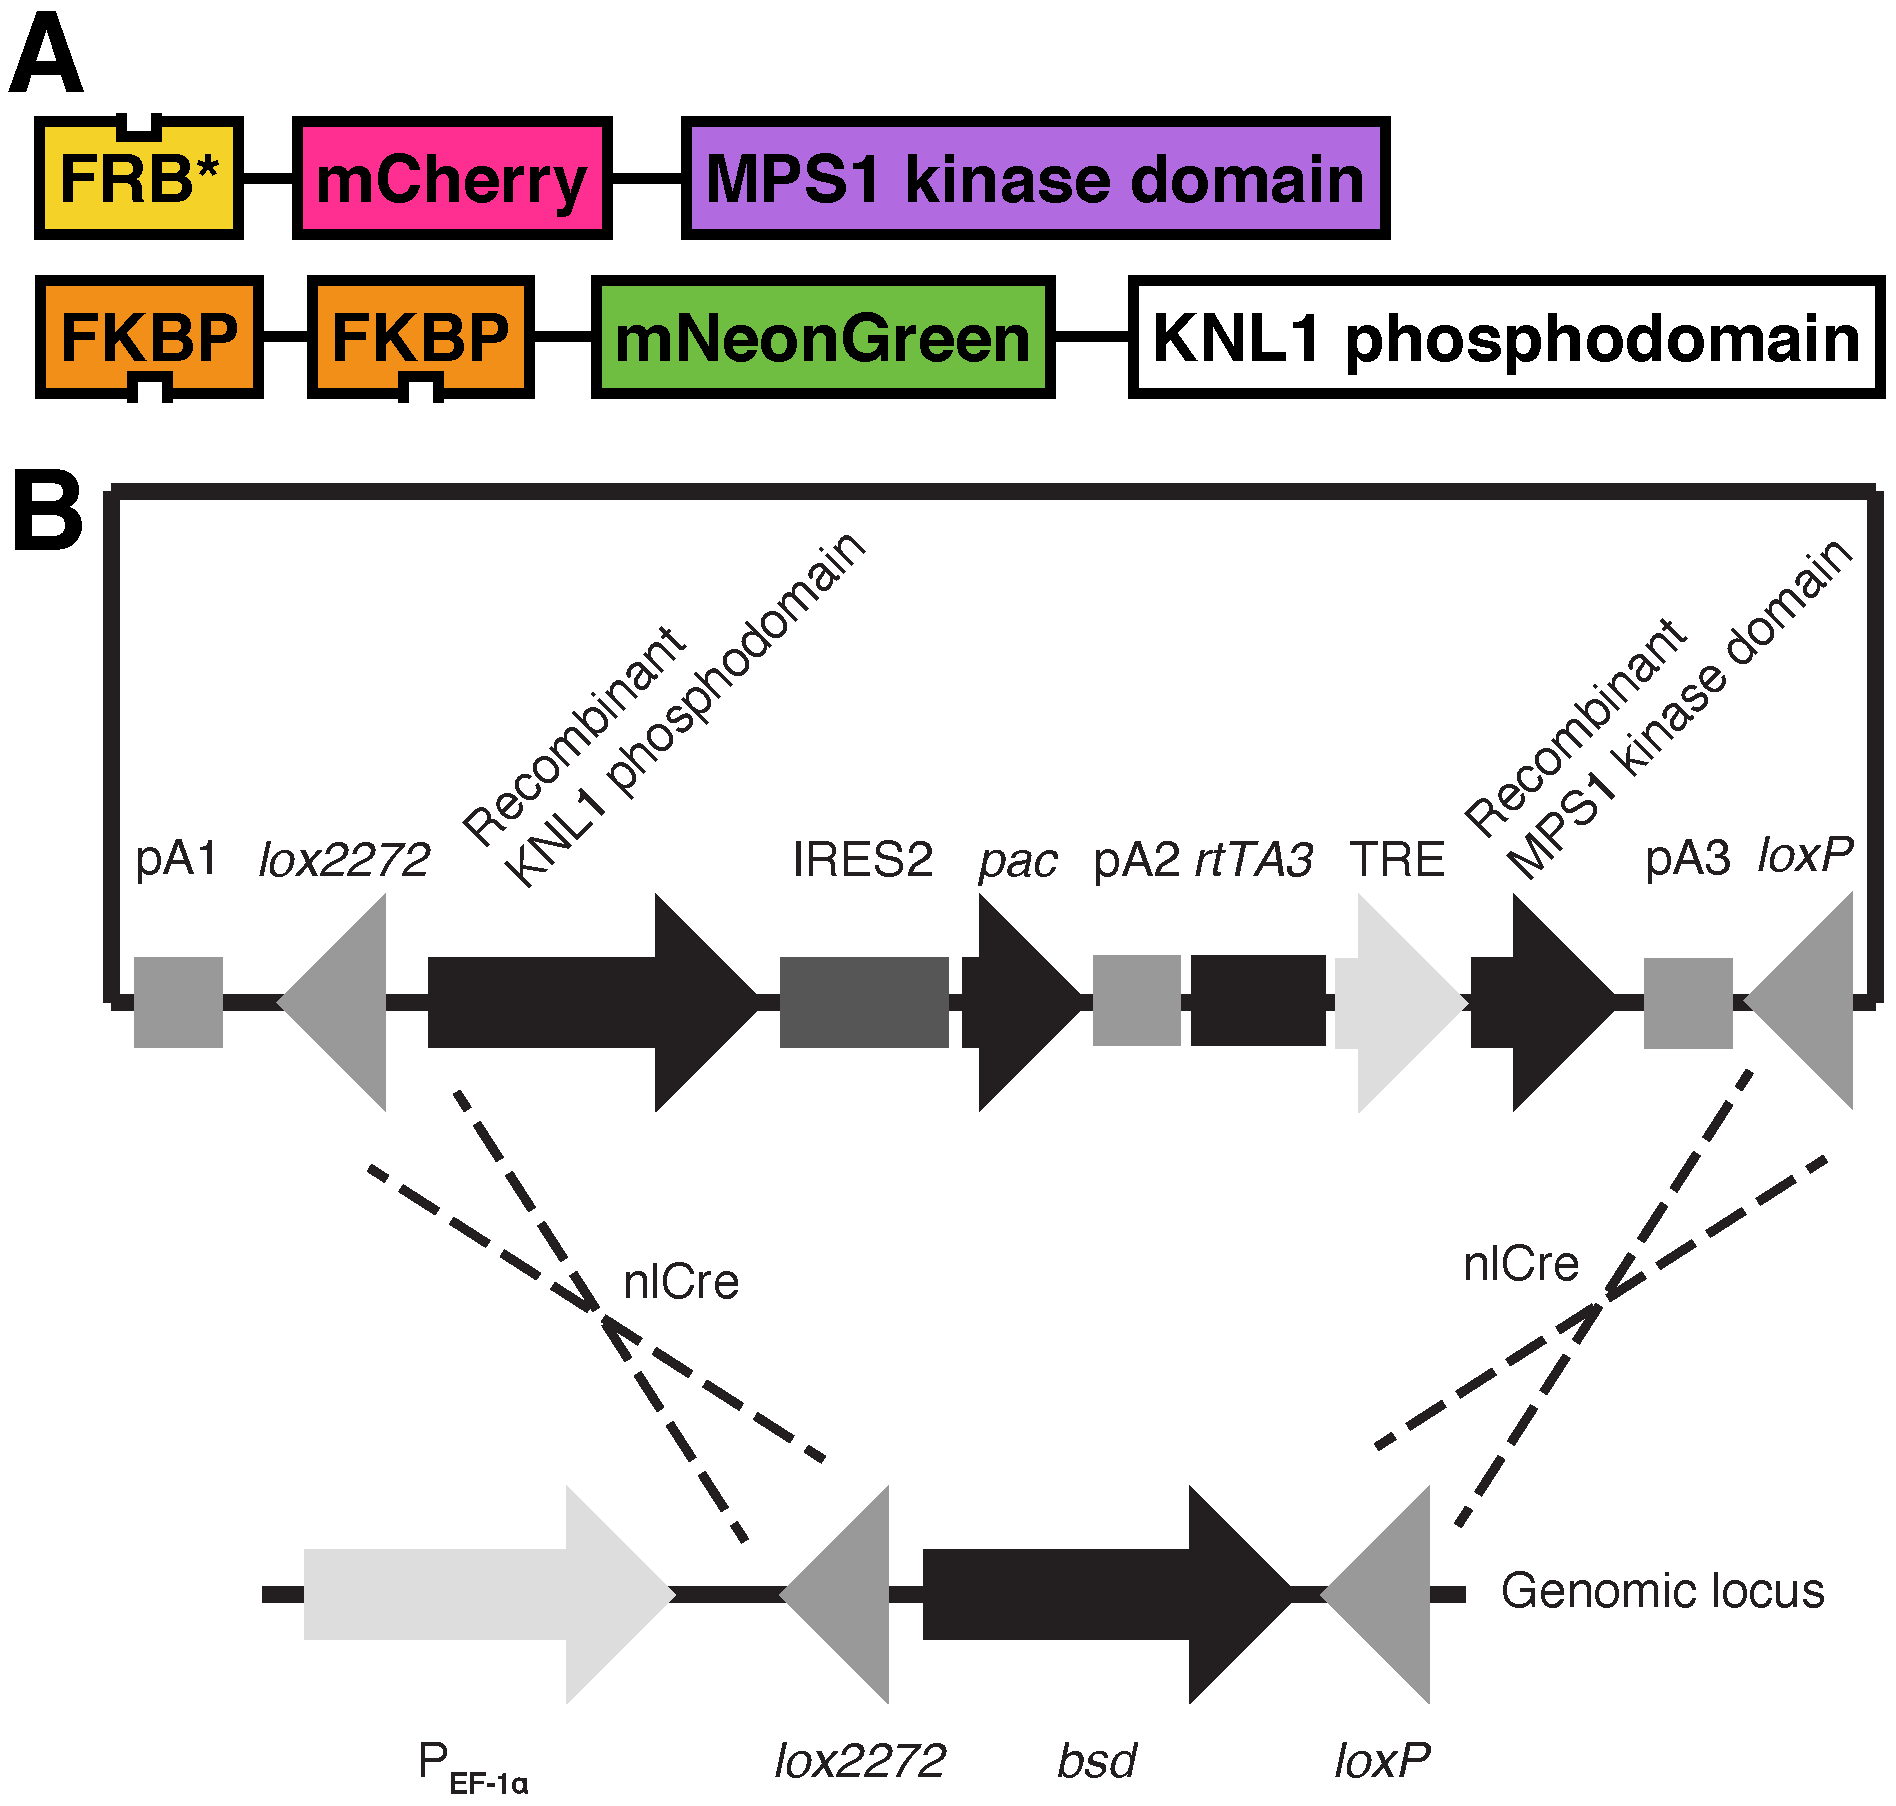
\includegraphics[width=0.7\textwidth]{chapters/figures/eSAC+Cre-lox.pdf}
    \phantomsubfiglabel{eSAC} % subfigure A
    \phantomsubfiglabel{Cre-lox} % subfigure B
    \caption{\textbf{The design of an ectopic SAC (eSAC) activator.}}
    \noindent\justifying (A) The eSAC activator consists of a recombinant \protein{Knl1} phosphodomain and a recombinant \protein{Mps1} kinase domain. The phosphodomain is at the N-terminus of the corresponding recombinant protein while the kinase domain is at the C-terminus of the corresponding recombinant protein. (B) A diagram demonstrating Cre-\bacterialgene{lox} recombination-mediated cassette exchange (RMCE) between a transfected circular plasmid (the top part) and the genomic locus (the bottom part). This diagram is not to scale. The design was adapted from \cite{HeLa-A12_Khandelia2011, HeLa-A12_Ballister2014}. pA1: the polyadenylation signal of herpes simplex virus thymidine kinase. IRES2: (encephalomyocarditis virus) internal ribosome entry site 2. \bacterialgene{pac}: the coding sequence of puromycin \textit{N}-acetyltransferase. pA2: the polyadenylation signal of bovine growth hormone. \textit{rtTA3}: an expression cassette encoding the reverse tetracycline-controlled transactivator 3 (rtTA3), consisting of the promoter of the human ubiquitin C gene, the coding sequence of rtTA3, and a polyadenylation signal from simian virus 40. TRE: a tetracycline-responsive promoter element consisting of six tandem tetracycline operators followed by the minimal promoter sequence derived from the human cytomegalovirus immediate-early promoter. pA3: the polyadenylation signal of rabbit \textbeta{}-globin. nlCre: nucleus-localized Cre recombinase. P\textsubscript{EF-1\textalpha{}}: promoter of the human \gene{EF1A} gene. \bacterialgene{bsd}: the coding sequence of blasticidin S deaminase. After integrated into the genomic locus, the recombinant phosphodomain is under the regulation of the \gene{EF1A} promoter while the recombinant kinase domain is under the regulation of the TRE. Colonies of stably-transfected cells selected by \SI{0.5}{\micro g/mL} -- \SI{2}{\micro g/mL} of puromycin in a well were pooled together to make an eSAC cell line.
    \label{eSAC+Cre-lox}
\end{figure}

The kinetochore targeting of \protein{Knl1} is mainly mediated by its C-terminus \cite{KNL1CTer_Kiyomitsu2007, Screpanti2011, Knl1CTer, MIS12CStructure_Petrovic2016, Spc105pCTer-MIND_Maskell2010} but may also be contributed by its N-terminus (\cite{eSAC}, Figure S1A and S1B by Dr. Ajit Joglekar and Palak Sekhri). Therefore, we fused different truncations of the \protein{Knl1} phosphodomain (in the middle of \protein{Knl1}) containing various numbers of MELT motifs with mNeonGreen (mNG, a bright monomeric yellow-green fluorescent protein \cite{mNG}) and FKBP. The kinetochore targeting of human \protein{Mps1} is mainly mediated by its N-terminus \cite{MPS1Localization_Ji, MPS1Localization_Hiruma, Mps1_Aravamudhan}. Therefore, we fused the kinase domain of \protein{Mps1} with FRB* \cite{FRB_T2098L} and mCherry. The fluorescent protein tags in the two recombinant proteins constituting the eSAC activator enabled convenient quantification of the eSAC concentration in real time at a single-cell level using fluorescence imaging.

The expression cassettes of the eSAC activator pair were stably integrated into the genome via Cre-\bacterialgene{lox} recombination-mediated cassette exchange (RMCE; \myref{Cre-lox}) \cite{HeLa-A12_Khandelia2011, HeLa-A12_Ballister2014}, wherein the expression of the recombinant \protein{Mps1} kinase domain is under the regulation of the Tet-On system. Fluorescence imaging revealed that the \protein{Knl1} phosphodomain does not display perceptible kinetochore localization (see Figure S1A of \cite{eSAC}). We next set out to test whether the exogenously expressed eSAC activator can indeed hijack the endogenous SAC signaling pathway and arrest mitotic cells in the metaphase in a rapamycin-dependent, kinetochore-microtubule attachment-independent manner.

\section{The eSAC activator works as intended}

As a proof of principle, we first tested (1) whether the recombinant \protein{Mps1} kinase domain can phosphorylate the recombinant \protein{Knl1} phosphodomain in the eSAC activator and (2) whether the phosphorylation reaction depends on rapamycin.

Using purfied proteins, we showed that the purified recombinant \protein{Mps1} kinase domain can phosphorylate the purified recombinant \protein{Knl1} phosphodomain in an in vitro kinase assay (\myref{KinaseAssay}). This reaction was strongly inhibited by reversine, an \protein{Mps1} inhibitor. The phosphorylation efficiency was higher when there was \SI{500}{nM} rapamycin in the reaction, but even without rapamycin, phosphorylation was still detectable by a phospho-specific antibody \cite{MELTActivity}. However, phosphorylation of the recombinant phosphodomain was undetectable in eSAC-expressing HeLa-A12 cells without the addition of \SI{500}{nM} rapamycin (\cite{eSAC}, Figure 2B by Adrienne Fontan), maybe because the concentrations of the purified recombinant \protein{Mps1} kinase domain and the purified recombinant \protein{Knl1} phosphodomain in the in vitro assay were higher than their concentrations in the cells. The addition of \SI{330}{nM} nocodazole also does not induce the phosphorylation of the recombinant \protein{Knl1} phosphodomain. Reciprocally, the MELT motifs in endogenous \protein{Knl1} were minimally phosphorylated when cells were treated with rapamycin. However, they were strongly phosphorylated in nocodazole-treated cells. Therefore, we concluded (1) that the recombinant \protein{Mps1} kinase domain phosphorylates the recombinant \protein{Knl1} phosphodomain in the presence of rapamycin and (2) that there is minimal crosstalk in the phosphorylation of the eSAC phosphodomain (by the recombinant \protein{Mps1} kinase domain) and the endogenous \protein{Knl1} (by the endogenous \protein{Mps1} localized at signaling kinetochores).

\begin{figure}
    \centering
    \includegraphics[width=0.95\textwidth]{chapters/figures/KinaseAssay.pdf}
    \caption{\textbf{The purified recombinant \protein{Mps1} kinase domain can phosphorylate the purified recombinant \protein{Knl1} phosphodomain in an in vitro kinase assay.}}
    \noindent\justifying (A) Phosphorylation of MELT\textsuperscript{13} was only detected when the kinase, the phosphodomain, and ATP co-existed in the reaction. (B) The phosphorylation reaction still happened even without the addition of \SI{500}{nM} rapamycin, probably because the concentrations of the purified recombinant \protein{Mps1} kinase domain and the purified recombinant \protein{Knl1} phosphodomain in this in vitro assay were higher than their concentrations in eSAC-expressing HeLa-A12 cells induced by \SI{2}{\micro g/mL} of doxycycline. The reaction was strongly inhibited by \SI{1}{\micro M} reversine, an \protein{Mps1} inhibitor.
    \label{KinaseAssay}
\end{figure}

Rapamycin (but not the vehicle DMSO) treatment resulted in metaphase arrest in eSAC-expressing HeLa-A12 cells (\myref{M6_DoseResponse}). Mutating MELT motifs (by mutating auxiliary T\textOmega{} sequences \cite{RecombinantKNL1, MELTActivity} and rendering the consensus MELT sequences non-phosphorylatable) of the recombinant phosphodomain prevented the rapamycin-induced metaphase arrest (\cite{eSAC}, Figure S2A by Dr. Ajit Joglekar and Palak Sekhri). A mass spectrometry analysis on the recombinant phosphodomain pulled down from lysates of eSAC-expressing rapamycin-treated cells identified peptides from \protein{Mps1}, \protein{Bub3}, and \protein{Bub1}, while the control group using eSAC-expressing cells arrested in mitosis by nocodazole could not (\cite{eSAC}, Figure 2F by Ian Whitney from Dr. Iain Cheeseman's group).

Together, these results supported that the recombinant \protein{Mps1} kinase domain phosphorylated MELT motifs of the recombinant \protein{Knl1} phosphodomain in the presence of rapamycin, which then recruits SAC proteins (like \protein{Bub3} and \protein{Bub1}) and delays anaphase onset in cells.

\section{Building a semi-automatic image analysis pipeline to enable the processing of large data sets}
\label{IncuCyteAnalysis}
For mitotic duration assays requiring live-cell time-lapse imaging, we utilized a semi-automatic pipeline [implemented in MATLAB (MathWorks)] to facilitate data analysis (\myref{DataAnalysisPipeline}). Images of fluorescence channel(s) were first pre-processed to remove backgrounds and corrected for shading. The background was obtained from a blank well containing only the imaging media. The shading pattern was calculated from a blank well containing the imaging media supplied with the corresponding purified fluorescence protein. Due to the lack of precise mechanical control of stage positioning on the IncuCyte\textsuperscript{\textregistered} ZOOM system [but not so much on the ImageXpress\textsuperscript{\textregistered} Nano Automated Imaging System (Molecular Devices) used in later chapters], there is non-negligible jittering over time. Images of the phase-contrast transmitted light channel were registered (aligned) with the preceding image in the stack recursively. The computed translations were then propagated to the calibrated fluorescence image stack(s).

Adherent mammalian cells typically assume a spherical shape from NEBD (nuclear envelop breakdown) to anaphase onset, while G\textsubscript{1}/S/G\textsubscript{2}/prophase cells usually assume a flattened shape on a plate. In slightly defocused phase-contrast transmitted light images, these cells appear as circles defined by the halo artifact \cite{PhaseContrastHalo}. Our semi-automatic pipeline utilized this to detect mitotic cells by convolving each image with kernels representing ``average'' mitotic cells (constructed by 2-D averaging of micrographs of manually picked mitotic cells of the same cell line). A threshold is then applied to the correlation matrix to convert it into a binary matrix. Connected components of high-correlation pixels (above a certain threshold of the pixel size) are recognized as mitotic cells. Centroids of these connected components were linked across successive frames to connect all frames of the same cell across the entire history from NEBD to anaphase onset (hereby defined as an ``event''). These events were then presented to the user in a graphical user interface (GUI), where the user can manually examine them carefully to either abandon a false event or to correct the frame index of NEBD/anaphase onset if necessary. The duration of mitosis is then calculated and corresponding $(t, x, y)$ coordinates are propagated to the fluorescence channel(s) to measure the fluorescence signal(s) of the cell.

\begin{figure}
    \centering
    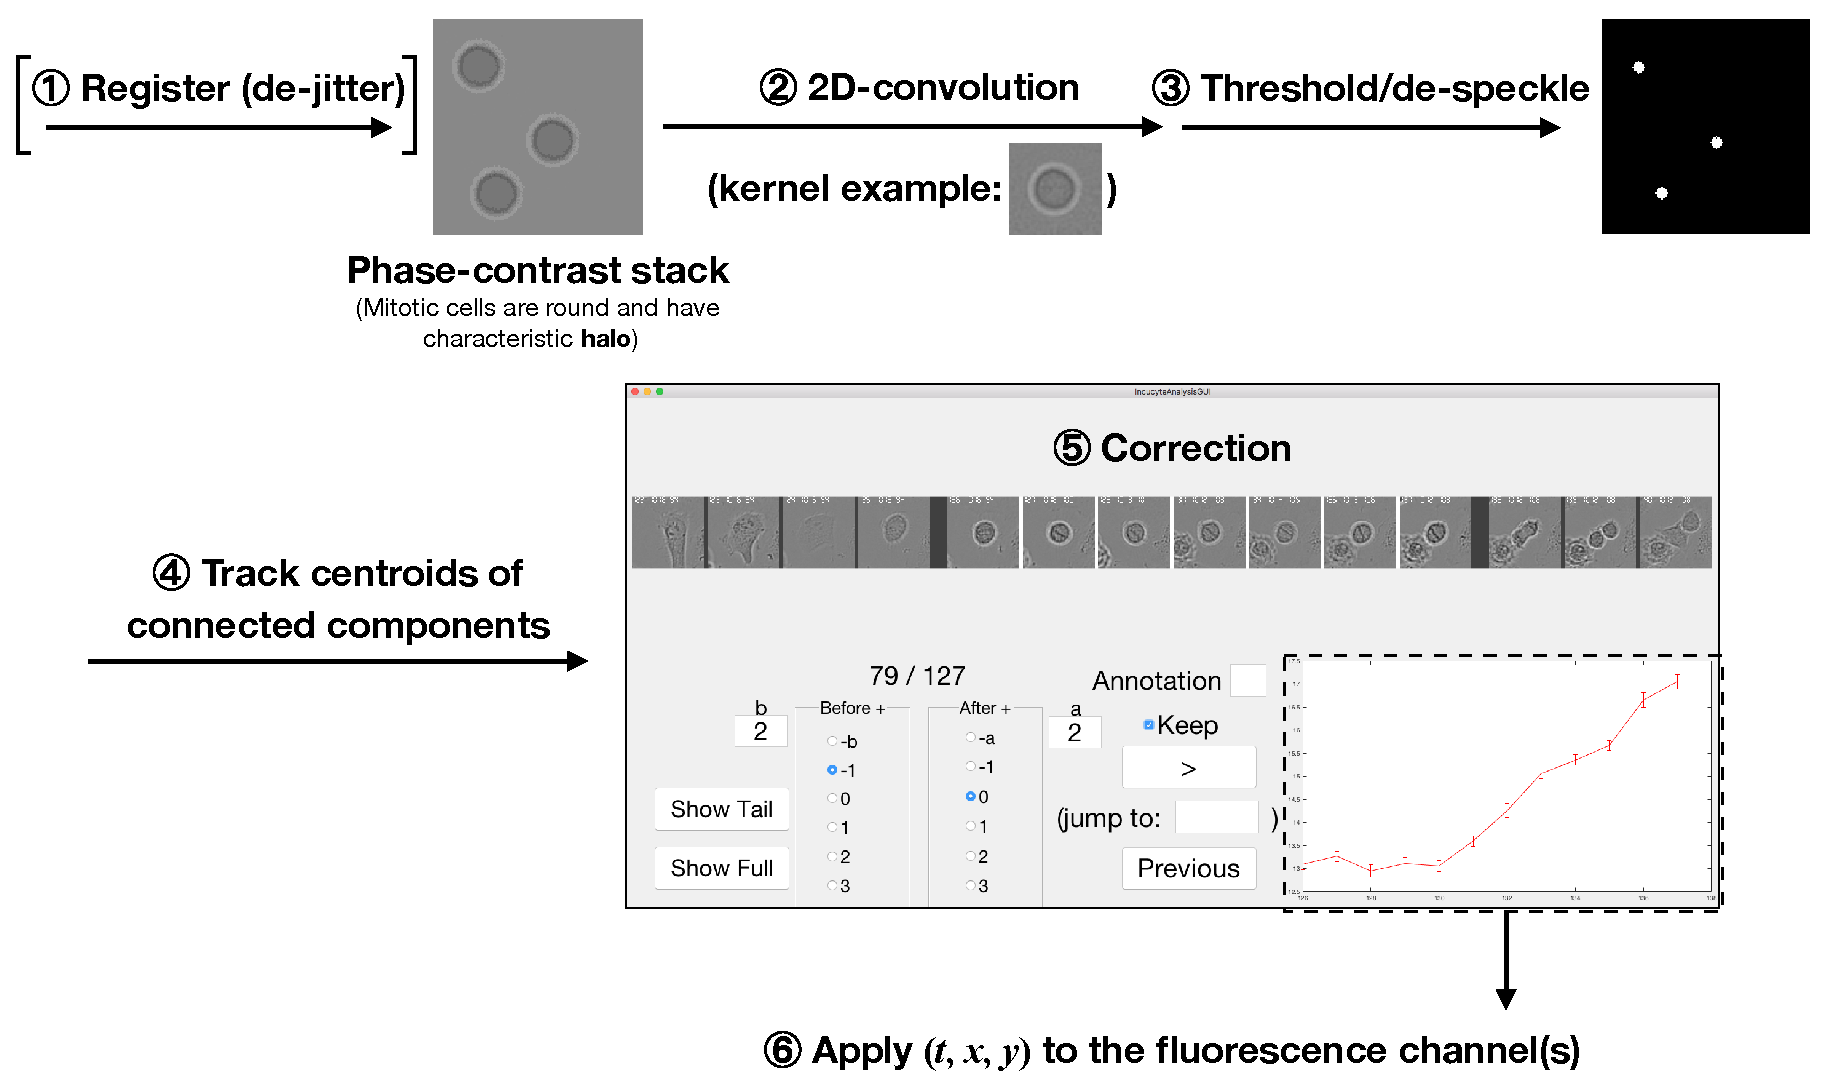
\includegraphics[width=0.95\textwidth]{chapters/figures/DataAnalysisPipeline.pdf}
    \caption{\textbf{A diagram illustrating the semi-automatic data analysis pipeline for mitotic duration assays.}}
    \label{DataAnalysisPipeline}
\end{figure}

\section{The eSAC activator reveals dose-response characteristics of the SAC}
The ability of the eSAC activator to hijack the endogenous SAC mechanism offered a novel tool to study the SAC quantitatively by correlating the cytosolic abundance of the eSAC activator with the mitotic duration from NEBD to anaphase onset (mitotic slippage) in a large population of cells. The first subject we explored was how the number of MELT motifs in the phosphodomain of \protein{Knl1} affects the signaling activity of the SAC (\myref{Summary_DoseResponse}). The idea has been explored in previous studies and came up naturally because there are 19 putative MELT motifs with various affinities to bind \protein{Bub1}-\protein{Bub3} in human \protein{Knl1} \cite{RecombinantKNL1, MELTActivity}.

\begin{figure}
    \centering
    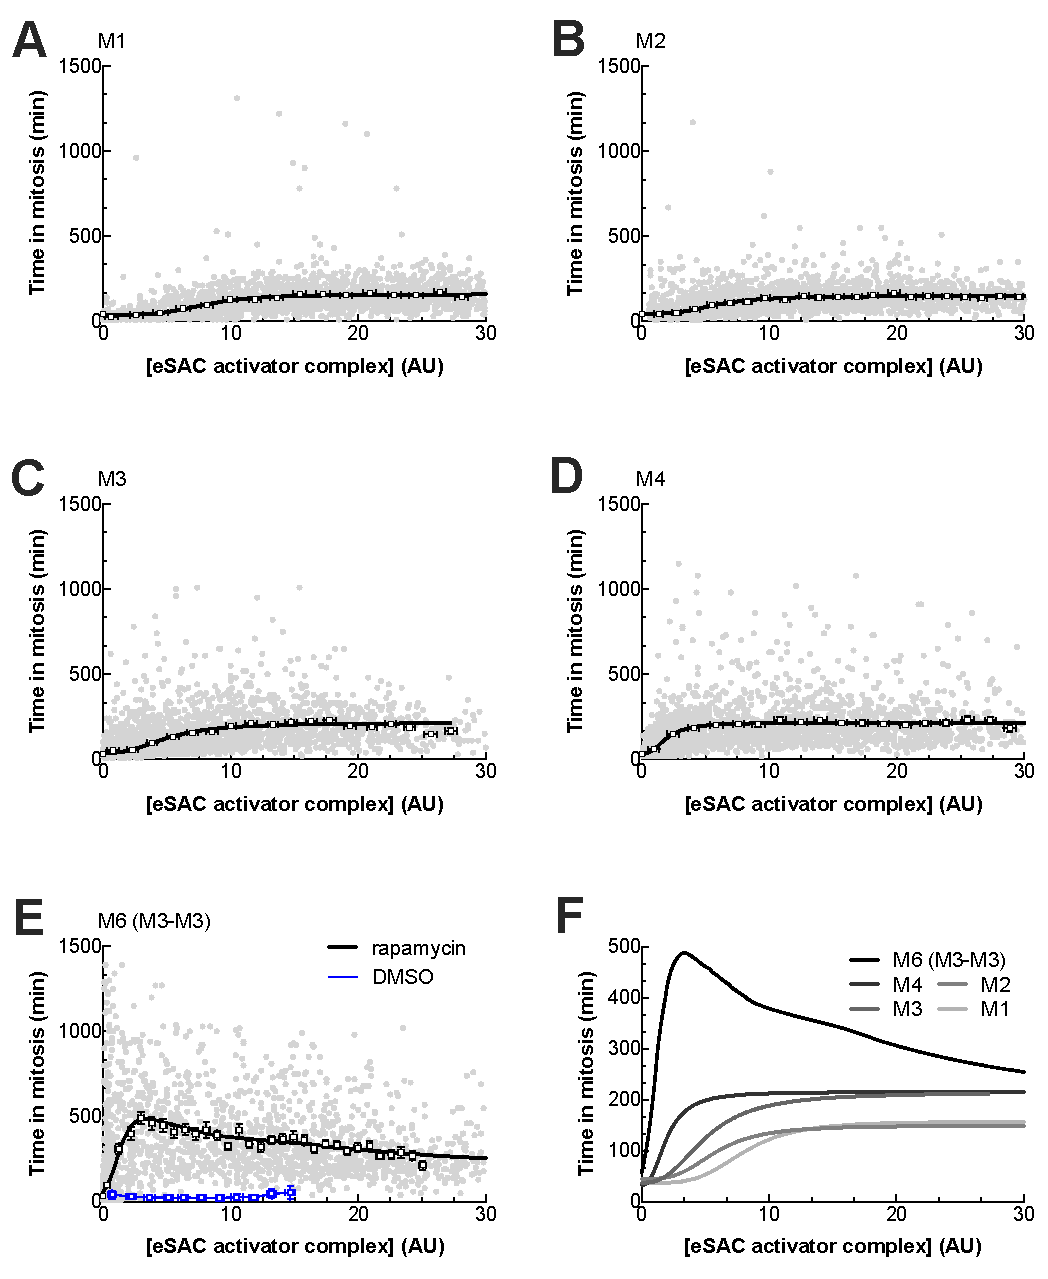
\includegraphics[width=0.7\textwidth]{chapters/figures/DoseResponse.pdf}
    \phantomsubfiglabel{M1_DoseResponse} % subfigure A
    \phantomsubfiglabel{M2_DoseResponse} % subfigure B
    \phantomsubfiglabel{M3_DoseResponse} % subfigure C
    \phantomsubfiglabel{M4_DoseResponse} % subfigure D
    \phantomsubfiglabel{M6_DoseResponse} % subfigure E
    \phantomsubfiglabel{Summary_DoseResponse} % subfigure F
    \caption{\textbf{A summary of the dose-response curves for the five eSAC activators with recombinant phosphodomains containing one to six MELT motifs.}}
    \noindent\justifying The dose (red fluorescence readout of the recombinant \protein{Mps1} kinase domain at the beginning of prometaphase in the cytosol of each cell) versus response (time in mitosis) relationship for different eSAC activators [(A) M1, (B) M2, (C) M3, (D) M4, and (E) M6 (M3-M3)]. Each gray dot represents a cell. Data from at least two independent experiments were compiled with more than \SI{2500}{} cells analyzed in each group. There may be some outliers beyond the range of the $x$- or $y$-axis (but they are included in the fitting). Bins of raw data (open squares, representing means $\pm$ SEMs) are overlaid. (F) shows a summary of the fitted dose-response curves for the five eSAC activators with recombinant phosphodomains containing one to six MELT motifs. Data from M1, M2, M3, and M4 are fitted to a Hill equation (see the main text) while LOESS (locally estimated scatterplot smoothing) was applied to show the trend of M6 (M3-M3). This figure is compiled and adapted from Figures 3C, 3E, 3F, 3G, 4B, and 4C of \cite{eSAC}. Dr. Ajit Joglekar, Adrienne Fontan, and Lauren Humphrey-Stark also contributed to setting up the experiments and/or performing data analysis.
    \label{DoseResponse}
\end{figure}

We started out by incorporating a single MELT motif (MELT\textsuperscript{12}, which is hereafter referred to as ``M1'', representing the minimal signaling unit of the core SAC signaling cascade) into the recombinant phosphodomain of the eSAC activator. We found that the duration of mitosis in the presence of \SI{500}{nM} rapamycin depended on the cytosolic abundance of the eSAC activator (\myref{M1_DoseResponse}). We used a Hill equation to fit these data, which displayed a sigmoidal trend:
\begin{equation*}
    \text{Time in mitosis} = m + \dfrac{M}{1+(\dfrac{K}{\text{[eSAC activator]}})^n},
\end{equation*}
wherein $n$ is the Hill coefficient and $K$ is the level of the eSAC activator at which the time in mitosis reaches the middle between the baseline level ($m$) and the plateau level ($m+M$).

Similar sigmoidal trends were also observed in dose responses of eSAC activators with recombinant phosphodomains containing two (MELT\textsuperscript{12}-MELT\textsuperscript{13}, hereafter referred to as ``M2''; \myref{M2_DoseResponse}), three (MELT\textsuperscript{12}-MELT\textsuperscript{14}, hereafter referred to as ``M3'' \cite{RecombinantKNL1}; \myref{M3_DoseResponse}), or four (MELT\textsuperscript{11}-MELT\textsuperscript{14}, hereafter referred to as ``M4''; \myref{M4_DoseResponse}) MELT motifs. The maximal mitotic duration for eSAC activators with recombinant phosphodomains containing one or two MELT motifs was the same, but it was higher for eSAC activators with recombinant phosphodomains containing three or four MELT motifs. Given that the eSAC activator recruits SAC proteins to arrest cells in metaphase, limited cytosolic abundance of one (or some) of the SAC proteins likely restricts the maximal mitotic duration (a metric of the signaling activity of the SAC), leading to a plateau at high abundance of the eSAC activator. This layer of restriction is coupled with diverse rates of MCC assembly, leading to various plateau levels for different recombinant phosphodomains (see \myref{ProzoneEffectModel,eSACDiscussions}). These results were consistent with a previous kinetochore-based study demonstrating that the \protein{Knl1} phosphodomain requires multiple MELT motifs to enable robust SAC signaling \cite{RecombinantKNL1}.

Surprisingly, the dose response of an eSAC activator with a recombinant phosphodomain containing six MELT motifs, which is made up of two tandem M3's and hereafter referred to as ``M6 (M3-M3)'' \cite{RecombinantKNL1}, featured a non-monotonic curve (\myref{M6_DoseResponse}). This eSAC activator induced a strong mitotic arrest at a low concentration. As the abundance of the eSAC activator complex increased, the signaling activity of the SAC gradually decreased.

\section{The distance between MELT motifs has a minor impact on the SAC activity}
There are two major differences between the M1, M3, and M6 (M3-M3) eSAC constructs in the previous section: (1) that the total number of MELT motifs in the signaling scaffold are different and (2) the lengths of these signaling scaffolds are different. Even though the phosphodomain of \protein{Knl1} is largely unstructured and flexible \cite{UnstructuredKNL1}, it remains to be seen whether the distance between MELT motifs affects the SAC activity. As a reference, the pair-wise distance between neighboring MELT motifs in the endogenous \protein{Knl1} are illustrated in \myref{PairwiseDistancesBetweenNeighboringMELTs}.

\begin{figure}
    \centering
    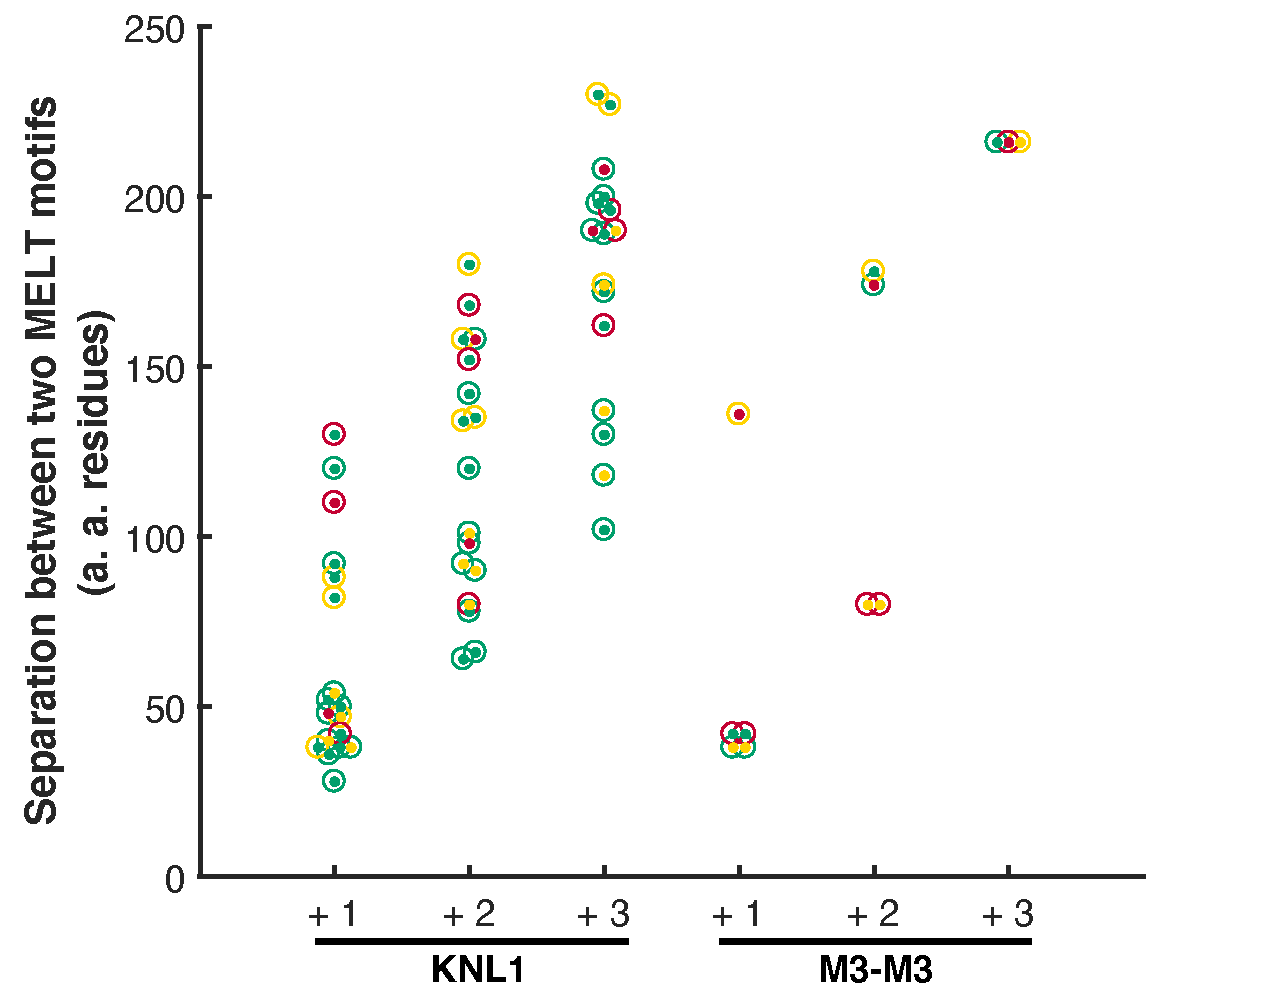
\includegraphics[width=0.6\textwidth]{chapters/figures/MELTSeparationColorCodedBeeSwarmPlot.pdf}
    \caption{\textbf{A beeswarm plot of pairwise distances between $(+1, +2, +3)$-neighboring MELT motifs in human \protein{Knl1} and the M6 (M3-M3) eSAC construct.}}
    \noindent\justifying Each ``circle \& center'' symbol represents a pair of neighboring MELT motifs. There are a total number of 19 putative MELT motifs in the endogenous \protein{Knl1} and 6 MELT motifs in the signaling scaffold of the M6 (M3-M3) eSAC construct. Therefore, we have a total number of $(18, 17, 16)$ pairs and $(5, 4, 3)$ pairs of $(+1, +2, +3)$-neighboring MELT motifs in the endogenous \protein{Knl1} and the M6 (M3-M3) eSAC construct, respectively. The coloring scheme follows the one in the original research \cite{MELTActivity} that studies the recruitment of \protein{Bub1} and is a rough estimation of the signaling activity of the corresponding MELT motifs (green: ``high'', yellow: ``intermediate'', red: ``low''). Distances in this chapter are measured between the Thr/Ser's of the consensus ``MELT'' sequences.
    \label{PairwiseDistancesBetweenNeighboringMELTs}
\end{figure}

To study the effect of the distance between MELT motifs in the signaling scaffold on the SAC activity, we designed a series of eSAC assays using artificially designed signaling scaffolds [MELT\textsuperscript{12}-$1\times$linker-MELT\textsuperscript{12}, MELT\textsuperscript{12}-$2\times$linker-MELT\textsuperscript{12}, and MELT\textsuperscript{12}-$3\times$linker-MELT\textsuperscript{12}]. The total number of MELT motifs are fixed (two) and the sequence of MELT motifs adopts that of MELT\textsuperscript{12}. Various copies of the endogenous linker between MELT\textsuperscript{11} and MELT\textsuperscript{12} are inserted between the two MELT\textsuperscript{12}'s. The resulting distance between the two MELT\textsuperscript{12}'s varies from 135 to 311 amino acids (\myref{DistanceEffect}), compared to a distance of 296 amino acids between the first motif and the last MELT motif in the M6 (M3-M3) construct in the previous section. From these assays, we observed that MELT\textsuperscript{12}-$3\times$linker-MELT\textsuperscript{12} has a slightly less SAC activity compared to the other two, but the difference is small and negative (about \SI{-15}{min} to \SI{-10}{min}) compared to the differences in the SAC activities between M1 and M6 (M3-M3) [as well as between M3 and M6 (M3-M3)]. Therefore, we inferred that the difference in the number of MELT motifs in the eSAC constructs is the major factor that determines its SAC activity.

\begin{figure}
    \centering
    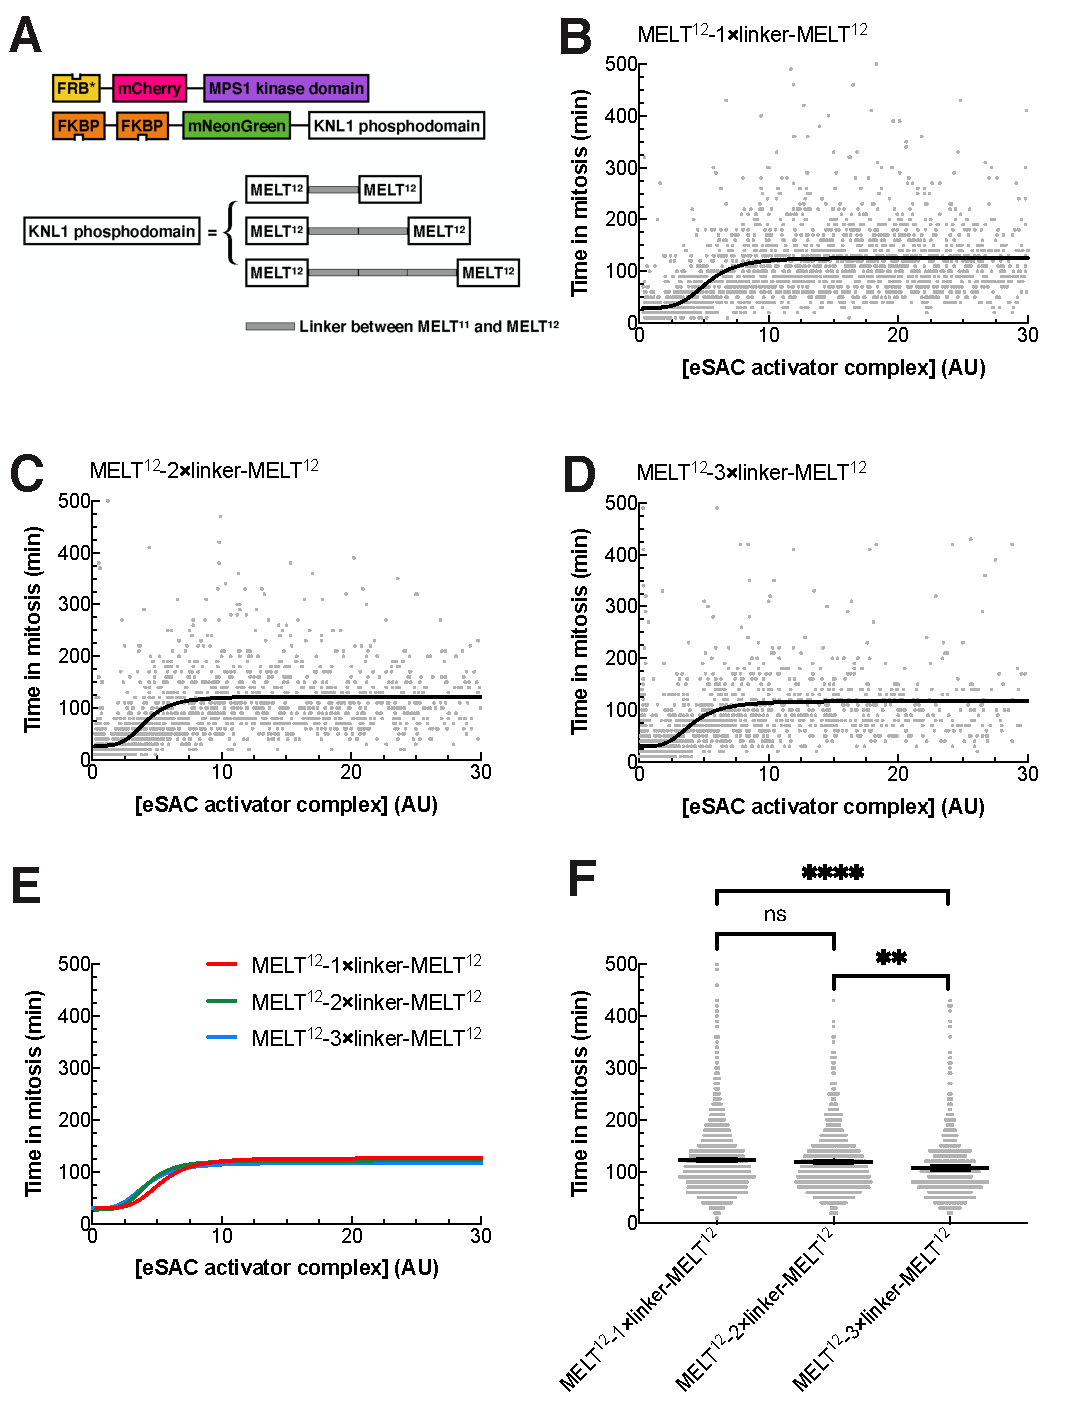
\includegraphics[width=0.7\textwidth]{chapters/figures/DistanceEffect.pdf}
    \caption{\textbf{The distance between MELT motifs has a minor impact on the SAC activity.}}
    \noindent\justifying (A) The distance between the two MELT\textsuperscript{12} motifs in the three constructs are 135, 223, and 311 amino acids, respectively [compared to a distance of 296 amino acids between the first motif and the last MELT motif in the M6 (M3-M3) construct in the previous section]. (B-E) A summary (E) of eSAC activities of MELT\textsuperscript{12}-$1\times$linker-MELT\textsuperscript{12} (B), MELT\textsuperscript{12}-$2\times$linker-MELT\textsuperscript{12} (C), and MELT\textsuperscript{12}-$3\times$linker-MELT\textsuperscript{12} (D) as the signaling scaffold. Each gray dot represents a cell. There may be some outliers beyond the range of the $x$- or $y$-axis (but they are included in the fitting).  (F) Comparison of the plateau levels of SAC response curves of the three eSAC constructs. Only cells with [eSAC activator] $> 10$ AUs are included. Data of more than 500 cells from two independent experiments were pooled for each group. The average mitotic durations are $(122.3 \pm 3.4)$, $(119.1 \pm 4.4)$, and $(108.1 \pm 5.7)$ minutes. Mean values $\pm 95\%$ confidence intervals are overlaid. Unpaired $t$-tests with Welch's correction were performed in Prism 9 (GraphPad Software).
    \label{DistanceEffect}
\end{figure}

\section{The dose-response data suggest cooperativity between multiple MELTs on a \protein{Knl1} phosphodomain that boosts the SAC signaling activity}
\label{ProzoneEffectModel}
We hypothesized that the increase in the maximum signaling activity of the recombinant \protein{Knl1} phosphodomain with multiple MELT motifs indicates synergistic signaling. This cooperativity model enables eSAC activator to assemble MCC at a higher rate than what independent signaling of the MELT motifs may sum up to. In fact, if each individual MELT motif on a recombinant \protein{Knl1} phosphodomain generates the MCC independently, the dose response of an eSAC activator with a recombinant phosphodomain containing a larger number of MELT motifs will simply approach the same plateau level of SAC activity at a lower concentration of the eSAC activator. This reasoning is especially evident when we compare the dose response of M3 (\myref{M3_DoseResponse}) eSAC versus the dose response of M6 (M3-M3, \myref{M6_DoseResponse}) eSAC.

As the concentration of the eSAC activator increases, they compete with each other to recruit SAC proteins from their limited pools in the cytosol. Individual eSAC activators, even with multiple phosphorylated MELT motifs, may not be able to bind multiple SAC proteins concurrently. Thus, the synergistic SAC signaling dwindles. This model explains the dramatic decline in the dose response of the M6 (M3-M3) eSAC activator at high concentrations (\myref{M6_DoseResponse}), which is reminiscent of the hook effect \cite{HookEffect}.

\section{Discussions}
\label{eSACDiscussions}
As an analogous system, the cytosolic eSAC activator provides a convenient approach to study the design of the core SAC signaling cascade quantitatively in mammalian cells. A previous study demonstrated that M6 (M3-M3) had similar SAC signaling activity to the endogenous human \protein{Knl1} phosphodomain (containing a total number of 19 putative MELT motifs) in Flp-In HeLa cells expressing LAP-\protein{Knl1} variants \cite{RecombinantKNL1}. Critical insights provided by dose-response data for eSAC activators with various recombinant phosphodomains hint on how the core signaling cascade of the SAC may adapt the signaling activity of each kinetochore based on the total number of signaling kinetochores in the cell.

Although the maximal response from the SAC signaling cascade saturates, its magnitude is not the same for all eSAC systems. This magnitude may be partially influenced by the rate of MCC assembly of various MELT motifs (the actual sequences of MELT\textsuperscript{11}, MELT\textsuperscript{12}, MELT\textsuperscript{13}, and MELT\textsuperscript{14} deviate from each other). A study published more recently from our lab on the sequence specificity of MELT motifs in Spc105 (the analog of human \protein{Knl1} in \Latin{Saccharomyces cerevisiae}) showed that replacing MELT motifs in Spc105 with those that bind to Bub1-Bub3 with a higher affinity reduces the possibility of chromosome missegregation but also slows down the progression of the cell cycle in the budding yeast \cite{YeastMELTSpecificity}. The evolution of MELT motif sequences may reflect a process of adjusting the balance between the accuracy of chromosome segregation and the propagation rate \cite{MELTEvolution}.

Using our dose-response data, we proposed a model for the biochemical design of the SAC signaling cascade. When there are a large number of signaling kinetochores in the cell (for example, right after NEBD), they compete with each other in recruiting SAC proteins from their limited pools in the cytosol. This competition masks cooperativity and the SAC activity per signaling kinetochore is weak. However, because the number of signaling kinetochores is large, the SAC signaling activity is high. When there are a few or even a single signaling kinetochores in the cell (for example, at a later stage of the prometaphase), each signaling kinetochore or even each \protein{Knl1} at signaling kinetochores can now recruit a large number of SAC proteins at the same time and cooperativity enables each remaining signaling kinetochores to assemble MCC at a high rate.

Unstable association between the recombinant \protein{Knl1} phosphodomain and the recombinant \protein{Mps1} kinase domain may introduce a source of noise. Therefore, we built upon the rapamycin-induced dimerization system to engineer our eSAC activator. However, endogenous \protein{Mps1} competes with microtubules to bind to the \protein{Ndc80} complex, thereby gaining spatial proximity to \protein{Knl1} at kinetochores \cite{MPS1Localization_Ji, MPS1Localization_Hiruma}. It is possible that the difference in the dynamics of \protein{Mps1} could potentially lead to observation of artifacts that do not apply to the endogenous SAC signaling cascade. Therefore, the model proposed here should be rigorously examined on kinetochore-based SAC signaling. This is the motivation of our study described in \myref{chpt:3}.

\section{Materials and Methods}
\subsection{Purification of the recombinant \protein{Mps1} kinase domain}
The recombinant bacmid encoding 6×His-MBP-TEV-FRB*-mCherry-\protein{Mps1}\textsuperscript{kinase domain} (\SI{124.8}{kDa}) was generated %from pCCB15
via Bac-to-Bac\textsuperscript{\textregistered} (Thermo Fisher Scientific). Baculovirus-transfected Sf9 cells (from \SI{1}{L} of culture) were pelleted down and stored at \SI{-80}{\celsius} until protein purification. Cells were resuspended in buffer IA [\SI{50}{mM} Tris-HCl (pH 7.5), \SI{300}{mM} NaCl, 0.2\% Triton X-100, \SI{20}{mM} imidazole, 0.1\% \textbeta-mercaptoethanol, and supplemented with PMSF and cOmplete\texttrademark{} EDTA-free Protease Inhibitor Cocktail (Roche) before usage] to a total volume of \SI{60}{mL}. Cells were lysed by a Dounce homogenizer (20 strokes using the loose pestle followed by 1 stroke using the tight pestle) supplied with Benzonase\textsuperscript{\textregistered} Nuclease (Sigma-Aldrich). Cell lysates were then centrifuged at \SI{18000}{rpm}, \SI{4}{\celsius} for \SI{45}{min} in a F21S-8x50y rotor. The supernatant was transferred and the pellet was discarded. \SI{5}{mL} of Ni-NTA agarose (equilibrated with buffer IA; Thermo Fisher Scientific) was added into the supernatant and the mixture was rotated at \SI{4}{\celsius} for \SI{3.5}{h}. The slurry was then washed with \SI{5}{mL} of buffer IA for 4 times. Bound proteins were eluted with buffer IB [\SI{50}{mM} Tris-HCl (pH 7.5), \SI{300}{mM} NaCl, 0.2\% Triton X-100, \SI{200}{mM} imidazole, 0.1\% \textbeta-mercaptoethanol].

\SI{2}{mL} of amylose resin was added (equilibrated with buffer IB; New England Biolabs) into eluted proteins from the Ni-NTA agarose column and the mixture was rotated at \SI{4}{\celsius} for \SI{2.5}{h}. The protein-bound amylose resin was then washed with \SI{5}{mL} of buffer IC [\SI{50}{mM} Tris-HCl (pH 7.5), \SI{300}{mM} NaCl, 0.2\% Triton X-100] for 4 times. \SI{2.5}{mL} of buffer IC followed by \SI{40}{\micro L} of \SI{1}{M} \textsc{d}-(+)-maltose stock solution was then added into the slurry. The mixture was rotated at \SI{4}{\celsius} for \SI{30}{min} and then eluted proteins were collected. The elution was loaded onto a Superdex 200 pg column (Cytiva) for size-exclusion chromatography. Fractions corresponding to the monomeric full-length 6×His-MBP-TEV-FRB*-mCherry-\protein{Mps1}\textsuperscript{kinase domain} (determined by molecular weight estimation and SDS-PAGE analysis) were subject to a subsequent Bradford protein assay (Bio-Rad Laboratories) and later used in the in vitro kinase assay.

\subsection{Purification of the recombinant \protein{Knl1} phosphodomain}
%pCCB9-
Transformed Rosetta\texttrademark{} 2(DE3) cells were induced to express 6×His-3×FLAG-TEV-MELT\textsuperscript{12-14}-mNeonGreen-2×FKBP (\SI{73.1}{kDa}) by \SI{1}{mM} IPTG at \SI{25}{\celsius} for \SI{20}{h}. Cells from \SI{2}{L} of Luria-Bertani liquid media were harvested, resuspended in deionized water into a total volume of \SI{40}{mL}, and then stored at \SI{-80}{\celsius} until protein purification.

The cell slurry was thawed on ice and an equal volume of $2\times$ buffer A [the $1\times$ buffer A has the following composition: \SI{50}{mM} Tris-HCl (pH 7.4), \SI{500}{mM} NaCl, \SI{0.1}{mM} EDTA, \SI{0.1}{mM} EGTA, and \SI{20}{mM} imidazole] supplemented with PMSF, \SI{0.1}{mg/mL} chicken egg white lysozyme (Sigma-Aldrich), \SI{2}{mM} DTT, and cOmplete\texttrademark{} EDTA-free Protease Inhibitor Cocktail was added into the slurry. Cells were lysed by sonication for a total amount of on time of \SI{150}{s} at 62\% amplitude (Model 500 sonic dismembrator, Thermo Fisher Scientific) in a water-ice bath at \SI{0}{\celsius}. Triton X-100 was added to a final concentration of 0.5\%. Lysates were rotated for \SI{15}{min} and then centrifuged at \SI{18000}{rpm}, \SI{4}{\celsius} for \SI{45}{min} in a F21S-8x50y rotor. The supernatant was filtered through 0.45-\textmu{}m syringe filter units (MilliporeSigma) and the pellet was discarded. \SI{1.5}{mL} of Ni-NTA agarose (equilibrated with buffer A supplemented with 0.1\% Triton X-100) was added into the filtered supernatant and the mixture was rotated at \SI{4}{\celsius} for \SI{3}{h}. The slurry was then washed with \SI{10}{mL} of buffer A supplemented with 0.1\% Triton X-100 for 4 times. Bound proteins were eluted with \SI{6}{mL} of buffer B [\SI{50}{mM} Tris-HCl (pH 7.4), \SI{500}{mM} NaCl, \SI{0.1}{mM} EDTA, \SI{0.1}{mM} EGTA, 0.1\% Triton X-100, and \SI{200}{mM} imidazole] for \SI{1}{h} at \SI{4}{\celsius}. The elution was filtered through a 0.45-\textmu{}m syringe filter unit and dialyzed in a Slide-A-Lyzer\texttrademark{} dialysis cassette (10K MWCO; Thermo Fisher Scientific) overnight against an imidazole-free buffer [\SI{50}{mM} Tris-HCl (pH 7.45 at \SI{4}{\celsius}) and \SI{300}{mM} NaCl] and then loaded onto a Superdex 200 pg column for size-exclusion chromatography. Fractions corresponding to the 6×His-3×FLAG-TEV-MELT\textsuperscript{12-14}-mNeonGreen-2×FKBP (determined by molecular weight estimation and SDS-PAGE analysis) were later used in the in vitro kinase assay.

\subsection{In vitro kinase assay}
The substrate 6×His-3×FLAG-TEV-MELT\textsuperscript{12-14}-mNeonGreen-2×FKBP was incubated with 6×His-MBP-TEV-FRB*-mCherry-\protein{Mps1}\textsuperscript{kinase domain} at \SI{30}{\celsius} for \SI{5}{min} -- \SI{2}{h} in the kinase buffer [\SI{10}{mM} Tris-HCl (pH 7.5), \SI{100}{mM} NaCl, \SI{10}{mM} \ch{MgCl2}, and \SI{1}{mM} DTT] supplemented with \SI{500}{nM} rapamycin and \SI{0.25}{mM} ATP. The reactions were stopped with the Laemmli Sample Buffer (supplemented with \textbeta-mercaptoethanol, Bio-Rad Laboratories). Phosphorylation of the substrate was detected by our custom-made anti-\Peptide{MEIpTRSHTTALEC} phospho-specific rabbit polyclonal antibody (GenScript). Equal inputs of the substrate and the recombinant kinase across different groups were validated by silver staining (Bio-Rad Laboratories).

\subsection{Cell culture and Cre-\bacterialgene{lox} recombination-mediated cassette exchange}
All HeLa-A12 cells were cultured in Dulbecco's Modified Eagle's Medium (DMEM, with high glucose and phenol red, without glutamine, sodium pyruvate, or HEPES; Gibco) supplemented with 22 mM of HEPES (Corning), 9\% (by volume) of fetal bovine serum (Corning), and $1\times$ GlutaMAX (Gibco). This medium is referred to as ``complete DMEM'' in the following context.

For Cre-\bacterialgene{lox} RMCE, Lipofectamine 3000 (Invitrogen) is used to co-transfect \SI{1.5}{\micro g} of a circular plasmid carrying the transgene cassette and \SI{50}{ng} of the circular pCAGGS-nlCre plasmid. \SI{0.5}{\micro g/mL} of puromycin was added \SI{1.5}{d} later for \SI{3}{d} to select for stably-transfected HeLa-A12 cells. Puromycin-resistant colonies were then pooled together and subject to further validation by genotyping and/or immunoblotting.

\subsection{live-cell imaging on the IncuCyte\textsuperscript{\textregistered} ZOOM system}
Long-term fluorescence imaging of eSAC cell lines was conducted using the IncuCyte\textsuperscript{\textregistered} ZOOM Live Cell Analysis System (Sartorius) equipped with a $20\times$ objective. Cells were seeded in 12-well BioLite cell culture-treated plates (Thermo Fisher Scientific) 2 days before imaging in complete DMEM supplemented \SI{2}{\micro g/mL} doxycycline. 30 -- 60 minutes prior to imaging, cells were washed once and FluoroBrite\texttrademark{} DMEM [supplemented with 9\% (by volume) of fetal bovine serum (Corning) and \SI{2}{\micro g/mL} doxycycline] with or without \SI{500}{nM} rapamycin were added. Phase-contrast and fluorescence images were acquired every \SI{10}{min} at fixed positions.% Images of the red and green fluorescence channels were acquired using a fixed exposure time of \SI{900}{ms} and \SI{300}{ms}, respectively.
\chapter{Enrichment of SAC Proteins at Kinetochores Strengthens the SAC Signaling Activity}
\label{chpt:3}

The model which we proposed in \myref{ProzoneEffectModel} relies on certain basic preconditions. First, the competition among a large but physiologically relevant number of phosphorylated MELT motifs in the cell for the limited pool of SAC proteins can effectively diminish freely diffusive SAC proteins in the cytosol. Second, the co-localization of multiple SAC proteins on the same \protein{Knl1} scaffold boosts the SAC signaling activity. Our follow-up studies described in this chapter corroborate these preconditions in a kinetochore-based setting, reinforcing the idea that cooperative synergy plays a critical role in the sensitivity of the SAC.

This chapter is tailored from two of my submitted first-(co)author manuscripts \cite{KImotifPaper, Paper3} with the inclusion of unpublished supplementary data (see \myref{HybridGenotypingdsDNA,5RACE}). Most figures are reproduced from the two manuscripts. I am the main contributor to all experiments except those in \myref{SACProteinKinetochoreRecruitment,BUBR1del432-484KTLocalization}, which are credited accordingly in the corresponding caption.

\section{Using CRISPR-Cas9-mediated genome editing to tag SAC genes with mNeonGreen \Latin{in situ}}
\label{TaggingSACProteins}

A common practice to study the functions of a protein is to knock down the endogenous protein by RNAi and then rescue the cells with a mutated or truncated protein ectopically expressed in the cells. This is henceforth referred to as a knockdown-rescue experiment.
%Transient transfection may offer poor consistency in the expression level across different cells or throughout a long time course.
This strategy may cause undesirable over-expression of SAC proteins, which affects the progression of mitosis \cite{Bub1Overexpression-AuroraBHyperactivation} (see also \myref{per_se}), depletes the cytosolic pool of the corresponding binding partner and impairs the SAC signaling activity \cite{Bub3Competition, FissionYeastSACRobustness, ATMPhosphorylatesMad1S214, MAD1Overexpression_Ryan2012}, or even induces cell death (our unpublished imaging data of HeLa-A12 cells).
% 20160614_pPS28_Bub1_BubR1_Cdc20 (IncuCyte data) or my BubR1-rescue time-lapse experiments on the left scope

To prevent over-expression and facilitate live-cell imaging of SAC proteins, we utilized CRISPR-Cas9-mediated genome editing to tag SAC genes with a fluorescent protein \Latin{in situ} \cite{CRISPRProtocol, Atlas}, which may better protect any endogenous transcriptional and translational regulations by preserving the introns and 5'/3'-untranslated regions (UTRs; see \myref{5RACE}). This chapter focuses on three proteins from different layers of the SAC recruitment cascade: \protein{Bub1}, \protein{BubR1}, and \protein{Mad1}. We fused mNeonGreen to the N-terminus (upstream of the first exon) of \gene{BubR1} and \gene{Bub1} as well as the C-terminus (downstream of the last exon and before the stop codon) of \gene{Mad1} to enabled live-cell fluorescence imaging. We chose to tag \gene{Mad1} at its C-terminus based on a previous report that large N-terminal tags may disrupt the localization of \protein{Mad1} to the corona \cite{CoronaActivatesSAC}. mNeonGreen is separated from the tagged protein by a short flexible linker (see \myref{CRISPRMethods}) so that the binding dynamics, functions, and turnover of the protein may be minimally affected. mNeonGreen has fast maturation kinetics (shorter than \SI{10}{min} at \SI{37}{\celsius} \cite{mNG}) compared to the turnover rates of \protein{BubR1} and \protein{Bub1} in nocodazole-arrested mitotic cells \cite{BubR1MitosisTurnover, Bub1MitosisTurnover}. These CRISPR-Cas9-edited cell lines can also serve as a reference for the endogenous expression of these SAC proteins for knockdown-rescue experiments (\myref{NewBUBR1Rescue} and the next chapter).

Band intensities from immunoblotting (\myref{WBValidation}) and genotyping PCR (\myref{GenotypingValidation}) suggested that a half of \protein{BubR1} proteins in mitotic mNG-\gene{BubR1} cells and slightly over a half of \protein{Mad1} proteins in mitotic \gene{Mad1}-mNG cells were tagged with mNeonGreen. Our genotyping PCR revealed only one band corresponding to the edited mNG-\gene{Bub1} allele (\myref{GenotypingValidation}). However, immunoblotting using three different antibodies consistently revealed the coexistence of both mNG-tagged and wildtype \protein{Bub1} proteins in mitotic mNG-\gene{Bub1} cells (\myref{siBUB1,simNG-siBUB1}). We suspected that the double-strand break induced by Cas9 may have induced unexpected chromosomal rearrangement at the \gene{Bub1} locus, rendering the ``wildtype'' allele unable to be amplified by the genotyping primers but still able to express the wildtype \protein{Bub1} protein.

To validate this, we conducted 5'-rapid amplification of cDNA ends (RACE) to sequence the 5' region of all \gene{Bub1} mRNAs in the mNG-\gene{Bub1} cells. As a control, We only detected wildtype \gene{Bub1} mRNAs from the host HeLa-A12 cell line. However, from the mNG-\gene{Bub1} cells, we identified both the mRNA translating into mNG-\protein{Bub1} as well as an mRNA that has an unexpected 5'-UTR (\myref{5RACE}). The open reading frame of this unexpected mRNA still encodes the wild-type \protein{Bub1} protein. The exact configuration of the probable chromosomal rearrangement is unknown because 5'-RACE can only reveal the sequence of the 5'-UTR but not where the genotyping primers are supposed to bind. Nonetheless, this likely explains why the genotyping primers could not amplify the ``wildtype'' allele.

\begin{figure}
    \centering
    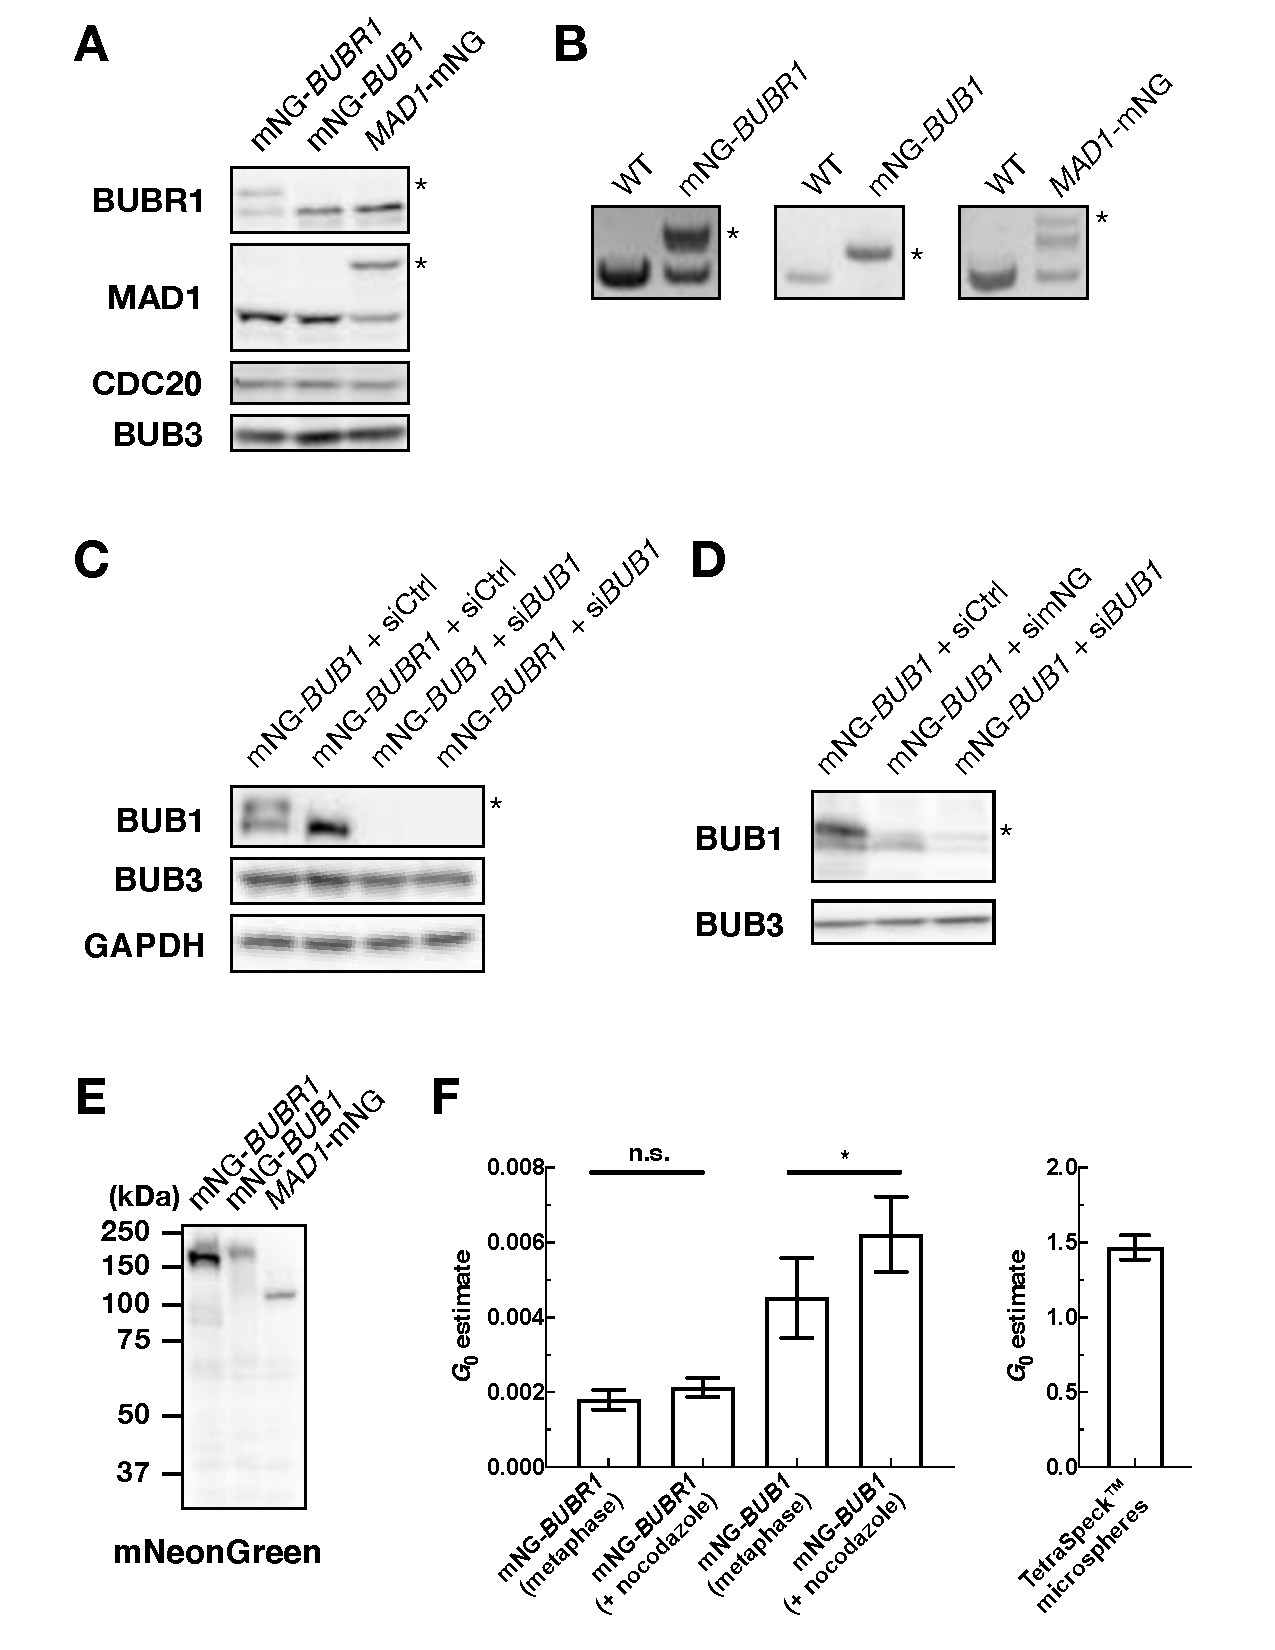
\includegraphics[width=0.99\textwidth]{chapters/figures/CRISPRValidation.pdf}
    \phantomsubfiglabel{WBValidation} % subfigure A
    \phantomsubfiglabel{GenotypingValidation} % subfigure B
    \phantomsubfiglabel{siBUB1} % subfigure C
    \phantomsubfiglabel{simNG-siBUB1} % subfigure D
    \phantomsubfiglabel{anti-mNG} % subfigure E
    \phantomsubfiglabel{FCS} % subfigure F
    \caption{Utilizing CRISPR-Cas9-mediated genome editing to fuse mNeonGreen to \gene{BubR1}, \gene{Bub1}, and \gene{Mad1} \Latin{in situ}.}
    \label{CRISPRValidation}
\end{figure}
\begin{figure}
    \noindent\justifying (Caption of \myref{CRISPRValidation} continued from a previous page) (A) Immunoblots of mitotic mNG-\gene{BubR1}, mNG-\gene{Bub1}, and \gene{Mad1}-mNG HeLa-A12 cells. Bands marked by asterisks correspond to proteins tagged by mNeonGreen. These blots are representative of three independent experiments. \protein{BubR1} bands were detected by horseradish peroxidase-catalyzed chemiluminescence. \protein{Mad1}, \protein{Cdc20}, and \protein{Bub3} bands were detected by fluorescent dye-conjugated secondary antibodies. \protein{Cdc20} and \protein{Bub3} levels in HeLa-A12 cells were not affected by the \Latin{in situ} tagging of \gene{BubR1}, \gene{Bub1}, or \gene{Mad1}. The weak bands below the strong wildtype bands in the \protein{Mad1} blot likely correspond to the alternatively-spliced \protein{Mad1\textbeta{}} \cite{Mad1beta}. (B) The genotyping (and subsequent sequencing) results verified the expected in-frame fusion of mNeonGreen. Bands marked by asterisks correspond to the mNeonGreen-tagged alleles. The middle bands from mNG-\gene{BubR1} and \gene{Mad1}-mNG cells were hybrid DNAs composed of one strand of the PCR product from the edited allele and one strand of the PCR product from the wildtype allele. These hybrid DNAs were thermodynamically less stable (\myref{HybridGenotypingdsDNA}). Adrienne Fontan also contributed here. (C) Immunoblots using lysates of the mNG-\gene{Bub1} HeLa-A12 cell line and another control genome-edited HeLa-A12 cell line revealed that \protein{Bub1} proteins in the mNG-\gene{Bub1} HeLa-A12 cell line were only partially tagged with mNeonGreen. Cells were treated with thymidine and then nocodazole overnight. The left two lanes were mitotic lysates harvested by mitotic shake-off while the right two lanes were pools of all cells (the fraction of cells in mitosis was significantly lower due to the knock-down of \gene{Bub1}). The immunoblot against \protein{Bub1} here was using a commercial rabbit antibody (see \myref{WBMethods}). (D) Knocking down \gene{Bub1} using a siRNA against mNeonGreen (simNG) or a siRNA against \gene{Bub1} (si\gene{Bub1}) confirmed that the lower band in the immunoblot against \protein{Bub1} is \protein{Bub1} (rather than due to cross-reactivity). The immunoblot against \protein{Bub1} here was using a commercial mouse antibody (see \myref{WBMethods}). We also tested another custom antibody from a previous study \cite{SheepAntiBUB1} and saw similar band patterns, further confirming that the lower band in the immunoblot against \protein{Bub1} corresponded to the wildtype \protein{Bub1}. (E) The majority of mNeonGreen-tagged proteins in mitotic mNG-\gene{BubR1}, mNG-\gene{Bub1}, and \gene{Mad1}-mNG HeLa-A12 cells were full length. The contribution of partial degradation or cleavage products to the fluorescence signal in \myref{FCS} is minor. (F) According to the FCS data, the metaphase concentration of mNG-\protein{BubR1} and mNG-\protein{Bub1} in the corresponding genome-edited HeLa-A12 cell line is $(2.4 \pm 0.4) \times 10^2$ nM and $(1.0 \pm 0.25) \times 10^2$ nM, respectively. Concentration measurements were calibrated by 0.1-\textmu{}m TetraSpeck\texttrademark{} microspheres with a nominal concentration of about \SI{0.30}{nM}. $G_0$, the auto-correlation at the 0-time lag, is inversely proportional to the average number of freely diffusive fluorescent proteins/particles in the excitation volume (see \myref{FCSMethods}). Each error bar represents the mean value $\pm$ the 95\% confidence interval of each group. Results were pooled from two independent experiments.
\end{figure}

\begin{figure}
    \centering
    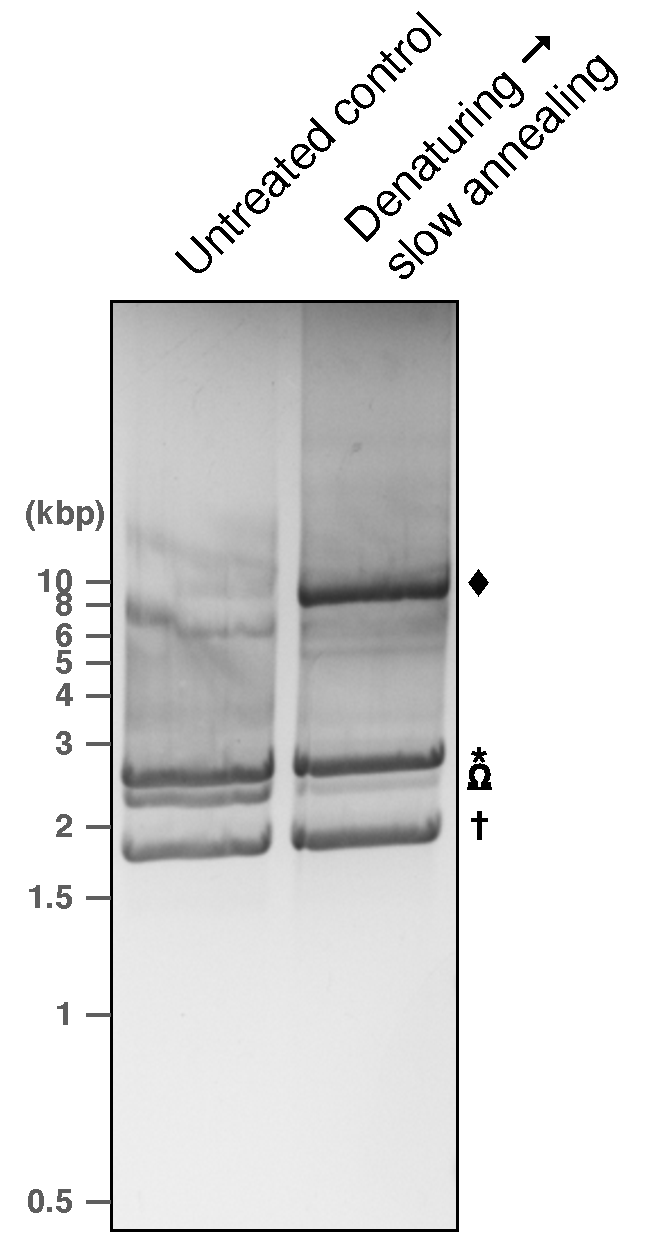
\includegraphics[width=0.3\textwidth]{chapters/figures/HybridGenotypingdsDNA.pdf}
    \caption{Genotyping PCR products (using the genome of the heterozygous mNG-\gene{BubR1} HeLa-A12 cell line as the template) feature hybrid double-stranded DNAs that are thermodynamically unfavorable.}
    \noindent\justifying Genotyping PCR products were purified using the GeneJET PCR Purification Kit (Thermo Fisher Scientific) and then equally split into 2 tubes. One of the tubes (right lane) was then placed in a boiling water bath for \SI{5}{min} and slowly cooled to room temperature, while the other tube (left lane) sit at room temperature. Diamond: likely to be a certain higher-order origami complex. Asterisk: the PCR product of the edited mNG-\gene{BubR1} allele (\SI{2519}{bp}, confirmed by sequencing). Cruciform: the PCR product of the wildtype \gene{BubR1} allele (\SI{1793}{bp}, confirmed by sequencing). \underline{\textOmega{}}: hybrid DNAs made up of one strand from the PCR product of the edited mNG-\gene{BubR1} allele and a complementary strand from the PCR product of the wildtype \gene{BubR1} allele. The identity of this band was also confirmed by sequencing (data not shown). Similar hybrid DNAs likely also existed in the purified \gene{Mad1}-mNG genotyping PCR products \myref{GenotypingValidation}.
    \label{HybridGenotypingdsDNA}
\end{figure}

\begin{figure}
    \centering
    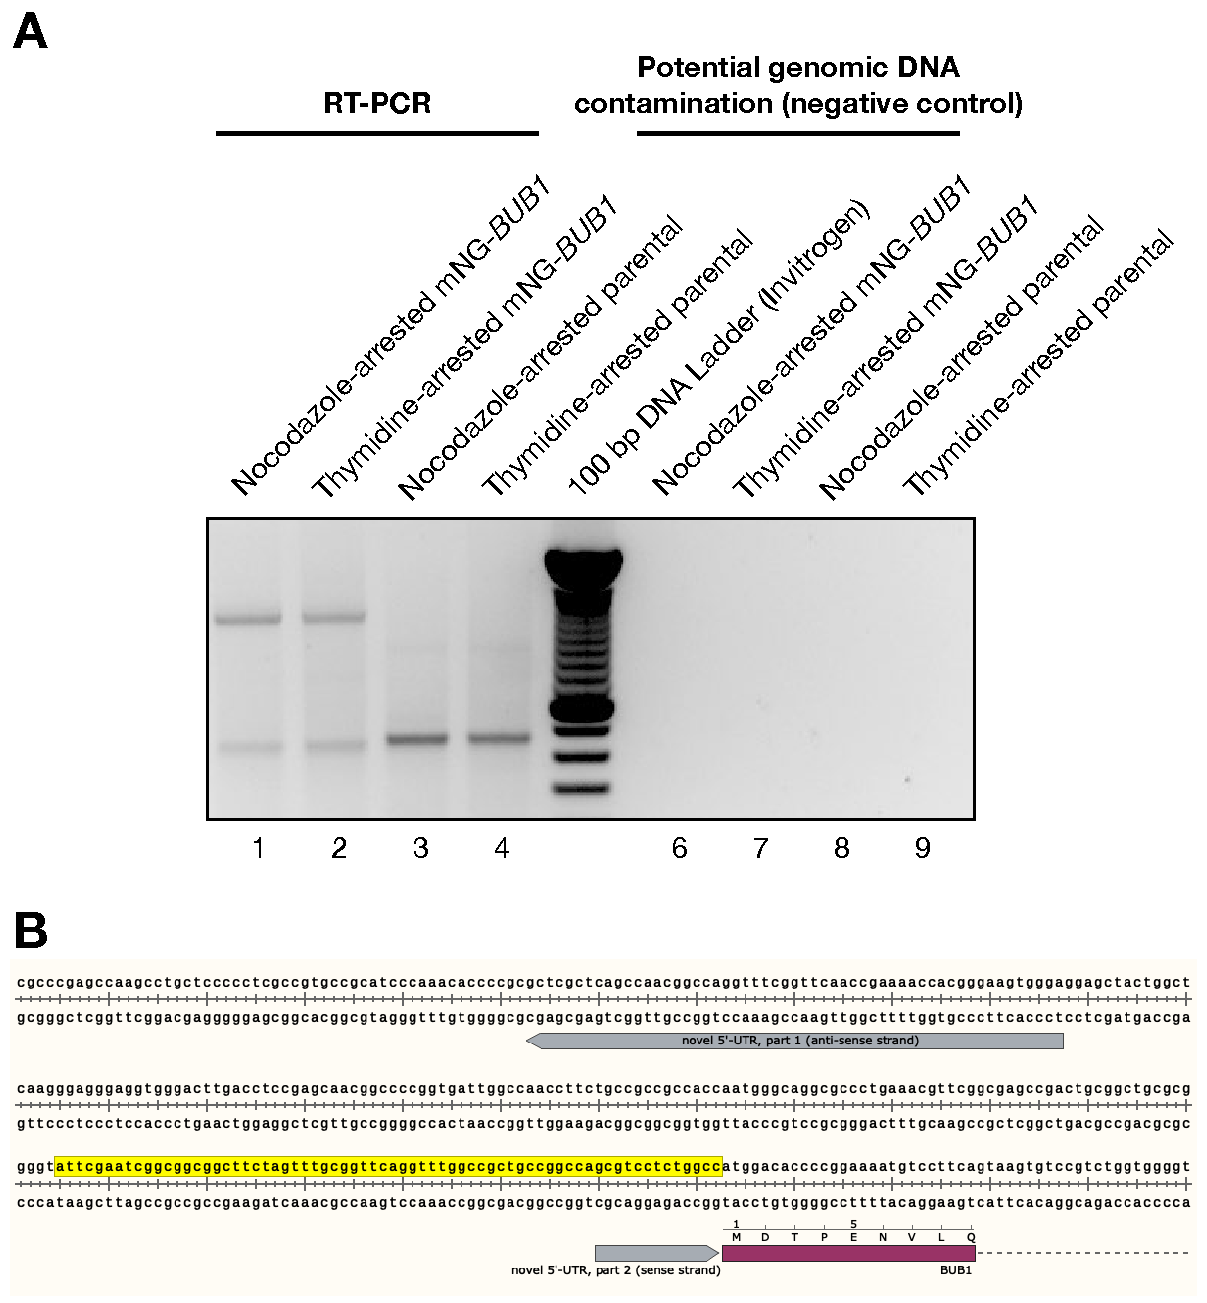
\includegraphics[width=\textwidth]{chapters/figures/5RACE.pdf}
    \phantomsubfiglabel{BUB1_5RACE} % subfigure A
    \phantomsubfiglabel{mNG-BUB1_5UTR_Seq} % subfigure B
    \caption{5'-RACE identifies the 5'-UTR sequences of different \gene{Bub1} alleles in the genome-edited mNG-\gene{Bub1} cell line.}
    \label{5RACE}
\end{figure}
\begin{figure}
    \noindent\justifying (Caption of \myref{5RACE} continued from a previous page) (A) 5'-RACE RT-PCR products using mitotic or G$_1$ total RNA extracts from the mNG-\gene{Bub1} genome-edited HeLa-A12 cell line (labeled as ``mNG-\gene{Bub1}'') or the host HeLa-A12 cell line (labeled as ``parental''). The right four lanes used purified total RNAs directly as the PCR templates without the reverse transcription reaction, which served as negative controls for any remaining genomic DNA that could affect the interpretation of these results. (B) The 5'-UTR of wild-type \gene{Bub1} mRNA (highlighted in yellow) identified from the host HeLa-A12 cell line and the 5'-UTR of the novel \gene{Bub1} mRNA identified from the mNG-\gene{Bub1} cells that still translates into the wildtype \protein{Bub1} protein (the two-part gray arrows). The 5'-UTR of the wildtype \gene{Bub1} mRNA is composed of -68 to -1 of the sense strand. The 5'-UTR of the novel \gene{Bub1} mRNA is composed of -206 to -260 of the anti-sense strand followed by -13 to -1 of the sense strand, which indicates a possible chromosomal rearrangement event. The 5'-UTR of the mRNA transcribed from the mNG-\gene{Bub1} allele (corresponding to the upper bands of the first 2 lanes on the left) is the same as the 5'-UTR of the mRNA transcribed from the wildtype \gene{Bub1} allele in the host HeLa-A12 cell line, confirming that our \Latin{in situ} tagging does not affect the transcription start site (TSS) of \gene{Bub1}. Different clones may have slightly varied TSSs (data not shown). For reference, the PAM sequence used in the initial CRISPR-Cas9-mediated genome editing spans from -19 to -17 of the sense strand. The nucleotide coordinates are based on the reference sequence (NC\_000002.12, chromosome 2 of the GRCh38.p13 primary assembly).
\end{figure}
% Some SAC genes like \gene{Mad1} \cite{Mad1beta} and \gene{Mad2} \cite{Mad2beta} are known to express splice variants with functional implications. Certain cell cycle-related kinases \cite{Nek2AlternativeSplicing} and phosphatases \cite{CDC25lternativeSplicing} were also reported to have coexisting splice variants with various expression profiles across different stages of the cell cycle.

\section{The recruitment of \protein{Bub1} to signaling kinetochores had a major depletion effect on the cytosolic pool of \protein{Bub1}}

To test whether the cytosolic pools of SAC proteins were depleted due to their recruitment to signaling kinetochores, we quantified the abundance of \protein{Bub1} and \protein{BubR1} in cells treated with either \SI{10}{\micro M} MG132 (a proteasome inhibitor which arrests mitotic cells in the metaphase independently of the SAC) or \SI{330}{nM} nocodazole. In MG132-treated cells, SAC proteins are mostly in the cytosol rather than recruited to the kinetochores \cite{MG132, Suijkerbuijk2012}. By comparing the cytosolic concentration of SAC proteins between cells treated with two different drugs, we can assess the depletion effect.
% Images from FCS?

Using fluorescence correlation spectroscopy (FCS), we estimated the cytosolic concentration of mNG-\protein{BubR1} and mNG-\protein{Bub1} in the corresponding MG132-treated HeLa-A12 cell line to be $(2.4 \pm 0.4) \times 10^2$ and $(1.0 \pm 0.25) \times 10^2$ nM, respectively (see \myref{anti-mNG,FCS}). Importantly, we confirmed that the cytosolic concentration of \protein{Bub1} in nocodazole-treated cells was significantly lower than that in MG132-treated cells, indicating that the recruitment of \protein{Bub1} to signaling kinetochores diminished the cytosolic pool of \protein{Bub1}. This effect was not statistically significant for \protein{BubR1}. One explanation could be that the cellular concentration of \protein{BubR1} is higher than \protein{Bub1}. Given that \protein{BubR1} is mainly recruited to signaling kinetochores by heterodimerizing with \protein{Bub1} and that the stoichiometry is $1:1$ \Latin{in vitro} \cite{BubBiochem}, the depletion effect is naturally less prominent. % especially when quantified by the auto-correlation at 0-time lag ($G_0$, which is inversely proportional to the average number of freely diffusive fluorescent proteins/particles in the excitation volume; see \myref{FCSMethods}).

\section{The numbers of \protein{BubR1}, \protein{Bub1}, and \protein{Mad1} recruited per signaling kinetochore are inversely correlated with the total number of signaling kinetochores in the cell}

A natural outcome of the depletion effect partially demonstrated in the previous section is that the number of SAC proteins recruited per signaling kinetochore will be inversely correlated with the total number of signaling kinetochores in the cell. Indeed, our previous measurement in the budding yeast \cite{Aravamudhan2016} proved this to be the case. To validate this in our genome-edited HeLa-A12 cells, we first need to obtain mitotic cells containing distinctly different numbers of signaling kinetochores.

To obtain mitotic cells with nearly all kinetochores activating the SAC, we treated mitotic cells with \SI{330}{nM} nocodazole, a drug that destabilizes microtubules. These nocodazole-treated cells resemble normal mitotic cells at the start of the prometaphase.

To obtain mitotic cells with a much smaller number of signaling kinetochores, we treated mitotic cells with GSK923295, a \protein{Cenp-E} inhibitor that impairs chromosome alignment \cite{GSK923295}. In these cells, usually a variable but smaller number of chromosomes are stranded near the spindle poles (\myref{SACProteinKinetochoreRecruitment_Images}). We analyzed only those cells that contained ten or less than ten polar chromosomes. Kinetochores on these polar chromosomes are either unattached or laterally attached, which activate the SAC \cite{GSK923295LateralAttachmentEM, GSK923295MonastrolCotreatment}. These GSK923295-treated cells arguably (see \myref{Chapter3Discussions}) resemble normal mitotic cells near the end of the prometaphase.

\begin{figure}
    \centering
    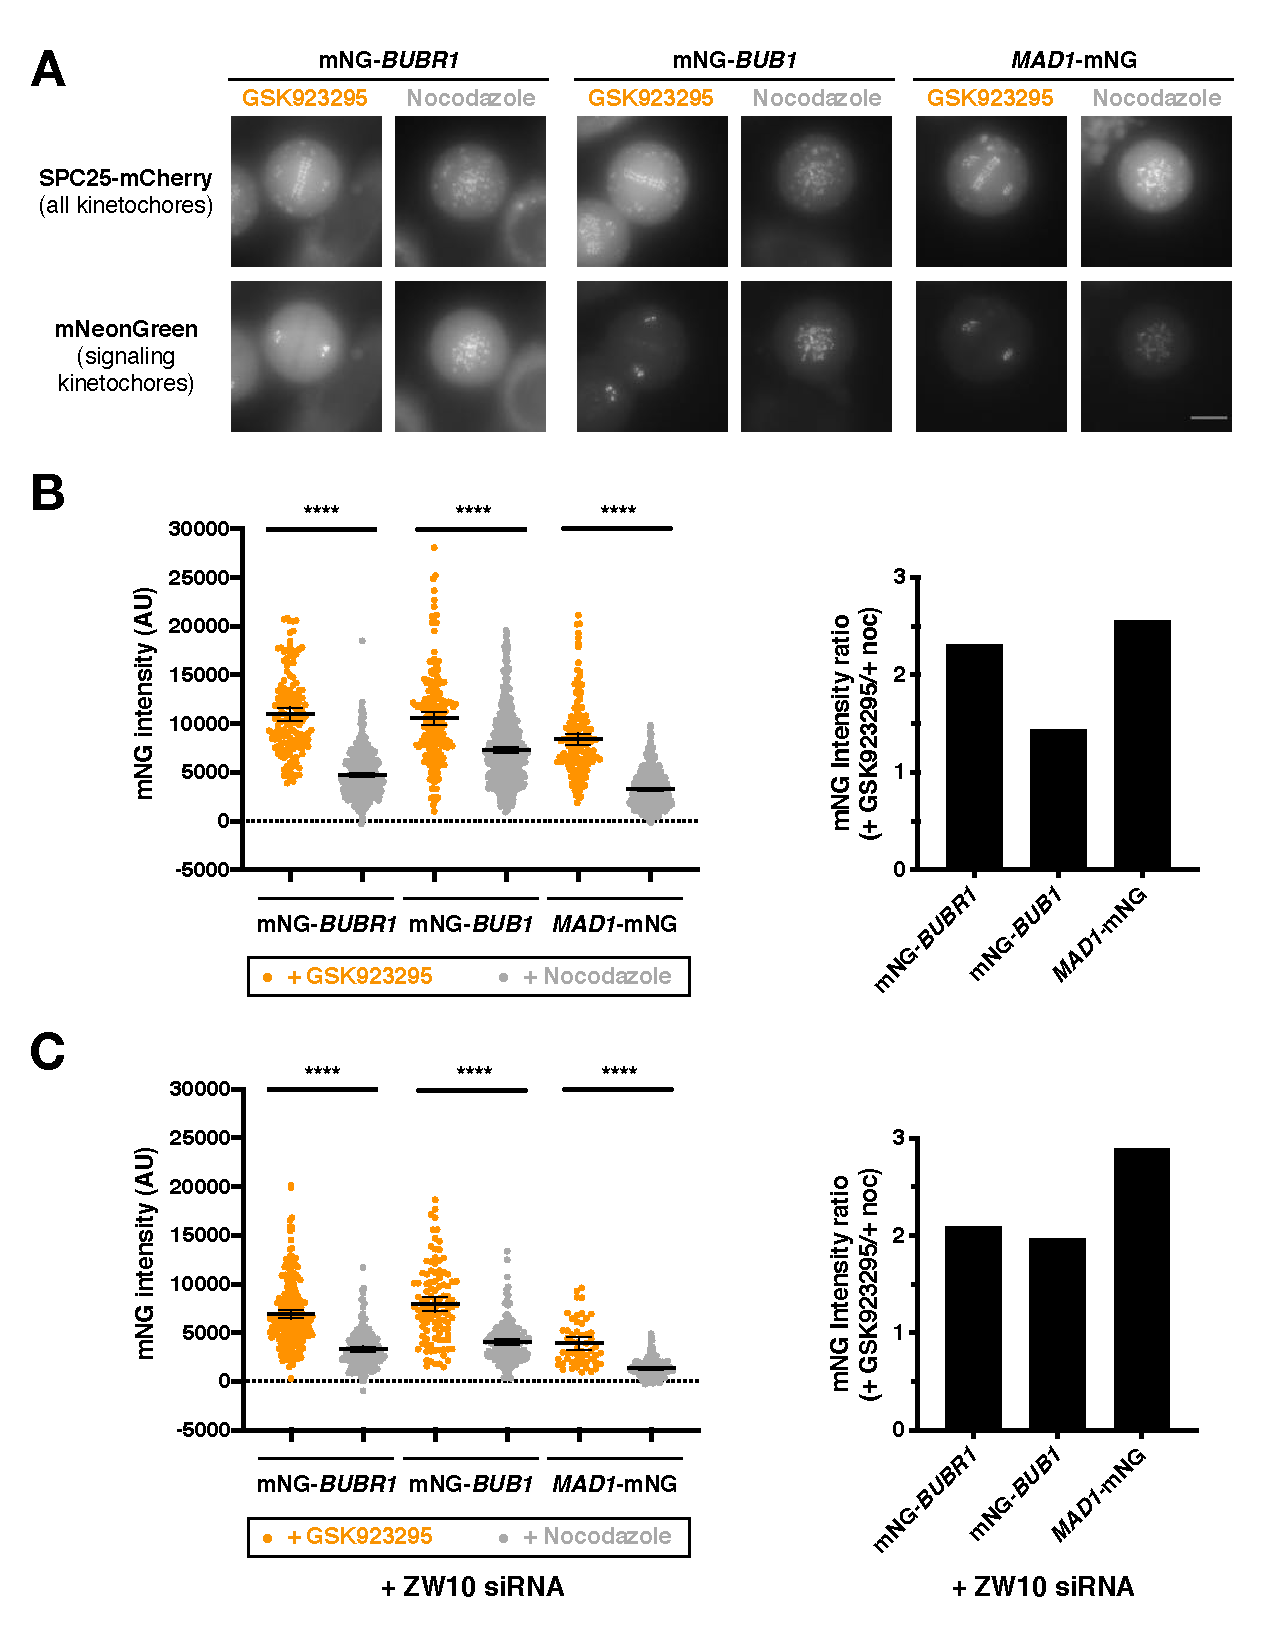
\includegraphics[width=0.95\textwidth]{chapters/figures/SACProteinKinetochoreRecruitment.pdf}
    \phantomsubfiglabel{SACProteinKinetochoreRecruitment_Images} % subfigure A
    \phantomsubfiglabel{SACProteinKinetochoreRecruitment_Quantification} % subfigure B
    \phantomsubfiglabel{siZW10SACProteinKinetochoreRecruitment_Quantification} % subfigure C
    \caption{The numbers of \protein{BubR1}, \protein{Bub1}, and \protein{Mad1} recruited per signaling kinetochore are inversely correlated with the total number of signaling kinetochores in the cell.}
    \label{SACProteinKinetochoreRecruitment}
\end{figure}
\begin{figure}
    \noindent\justifying (Caption of \myref{SACProteinKinetochoreRecruitment} continued from a previous page) Lauren Humphrey-Stark performed all imaging experiments and data analysis involved in this figure. (A) Representative micrographs showing cells from the three genome-edited HeLa-A12 cell lines treated with nocodazole or GSK923295. \protein{Spc25}-mCherry labeled all kinetochores \cite{Kukreja2020}. The coding sequence of \protein{Spc25}-mCherry was integrated into the genome of these HeLa-A12 cell lines immediately downstream of the constitutive \gene{EF1A} promoter (see \myref{Cre-lox}). Brightness and contrast have been adjusted but the LUT for each channel (row) is universal for different groups (column). Scale bar, \SI{10}{\micro m}. (B) Left panel: quantification of mNeonGreen signals at individual signaling kinetochores from experiments illustrated in (A). Each dot represents the measurement from one signaling kinetochore. Error bars represent 95\% confidence intervals of the mean. Results from at least two independent experiments are shown. Right panel: Pairwise ratios between the average mNeonGreen signals at individual signaling kinetochores of GSK923295-treated cells and nocodazole-treated cells in the left panel. (C) Similar to (B), except that all cells were additionally treated with a siRNA against \gene{ZW10}.
\end{figure}
% normalized by the average kinetochore-localized signal acquired in \Latin{in situ} tagged HeLa-A12 cells treated with nocodazole.

In nocodazole-treated cells, the number of mNG-\protein{BubR1} and \protein{Mad1}-mNG proteins recruited per signaling kinetochore in nocodazole-treated cells was lower than that of mNG-\protein{Bub1} recruitment (\myref{SACProteinKinetochoreRecruitment_Quantification}). Importantly, \protein{BubR1}, \protein{Bub1}, and \protein{Mad1} recruitment per signaling kinetochore were all significantly increased when cells were treated with GSK923295 compared to nocodazole (\myref{SACProteinKinetochoreRecruitment_Quantification}). This confirms that the number of SAC proteins recruited per kinetochore is indeed inversely correlated with the number of signaling kinetochores in the cell.

In human cells, \protein{Mad1} is also recruited to the fibrous corona around a signaling kinetochore \cite{RZZ-MAD1vsBUB1-MAD1_2015, RZZ-MAD1vsBUB1-MAD1_2018}, which may contribute to the measurement in \myref{SACProteinKinetochoreRecruitment_Quantification} through widefield fluorescence microscopy. The corona is mainly composed of the ROD-Zwilch-ZW10-Spindly (RZZS) complex \cite{RZZS_Sacristan2018, RZZS_Raisch2022}. A previous study found conflicting dependency of the kinetochore localization of \protein{BubR1} on the RZZS complex in \Latin{Xenopus} extracts versus HeLa cells \cite{BUBR1_XenopusVSHeLa}. Another study observed that the kinetochore localization of \protein{BubR1} and \protein{Bub1} in the presence of \SI{660}{nM} nocodazole even increased when cells were treated with a siRNA against \gene{ROD} (see Figure 1E of \cite{siROD_Zhang2019}).

To dissect how much the core SAC pathway contributes to the recruitment of these SAC proteins at signaling kinetochores, we knocked down \gene{ZW10}, a subunit of the RZZS complex, by a siRNA against \gene{ZW10}. We then quantified the recruitment of the mNG-labeled SAC proteins to signaling kinetochores as before. Consistent with previous studies \cite{CENPELocalization-BUBR1,siROD_Zhang2019}, \protein{Mad1} recruitment was significantly lower in both GSK923295 and nocodazole-treated cells when the RZZS complex was knocked down (\myref{siZW10SACProteinKinetochoreRecruitment_Quantification}). The number of \protein{BubR1} and \protein{Bub1} molecules recruited per signaling kinetochore was also reduced, which deviates from previous studies. We hypothesized that unlike our \Latin{in situ} tagging, the immunofluorescence labeling used in the quantification of the kinetochore localization of \protein{BubR1} and \protein{Bub1} \cite{BUBR1_XenopusVSHeLa,siROD_Zhang2019} may be additionally affected by the accessibility of the antigen (\protein{BubR1} and \protein{Bub1}) to the corresponding antibody. Such accessibility could be increased by the removal of the fibrous corona on the periphery of kinetochores.

Importantly, our data showed that the number of SAC proteins recruited per signaling kinetochore was still inversely correlated with the total number of signaling kinetochores in a cell when \gene{ZW10} was knocked down. This indicated that the competition between signaling kinetochores for the limited pool of SAC proteins in a cell persisted even when only the core SAC signaling pathway was functional.

\section{The equilibrium between the activity of \protein{Mps1} and counteracting phosphatases at signaling kinetochore is the same in nocodazole- and GSK923295-treated HeLa-A12 cells}
\label{MPS1sen-KTSection}

The observed difference in the recruitment of SAC proteins on a per kinetochore basis in nocodazole- and GSK923295-treated cells may be alternatively attributed to different degrees of phosphorylation of MELT motifs. This could be an indirect result of the various effect of different drugs on the kinetochore-microtubule attachment (see Figure 3f of \cite{Rheostat}). It may also be due to previously uncharacterized regulations of different drugs imposed on the activity of kinases and counteracting phosphatases at the kinetochore directly.

To test this alternative hypothesis in the HeLa-A12 cell line, we probed the equilibrium between the activity of kinases (mainly \protein{Mps1}) and counteracting phosphatases at the kinetochore (henceforth referred to as ``\protein{Mps1}'s activity'' for simplicity) using a similar phosphorylation sensor (MPS1sen-KT; see \myref{MPS1sen-KT_Scheme}) to the one developed in a previous study \cite{MPS1senor}. The original idea of this F{\"{o}}rster resonance energy transfer (FRET) sensor design was first proposed in \cite{FHA2BasedFRETSensorOriginalStudy}. The equilibrium between the activity of kinases and counteracting phosphatases determines the phosphorylation level of the substrate. If the substrate has a higher level of phosphorylation, FHA2 (the phospho-threonine binding domain from the yeast protein Rad53p) will have a higher affinity to bind to the substrate, thereby distancing the donor and the acceptor better and resulting in lower FRET efficiency. The expression cassette of the recombinant sensor is under the regulation of TRE and stably integrated into the genome of HeLa-A12 cells via Cre-\bacterialgene{lox} RMCE. The acceptor and the donor have a fixed $1 : 1$ stoichiometry by design and the recombinant sensor was mostly intact in the cell (with no major partial degradation species like mScarlet-I-\protein{Spc24} alone; see the immunoblot in \myref{MPS1sen-KT_Images}). Therefore, the ratio between the green channel readout and the raw FRET channel readout (even without corrections for the cross-excitation of the acceptor and the bleed-through of donor fluorescence) can be employed as a normalized measurement of the FRET efficiency (see \myref{FRETMetricTheory}) and serve as an indicator of \protein{Mps1}'s activity.

\begin{figure}
    \centering
    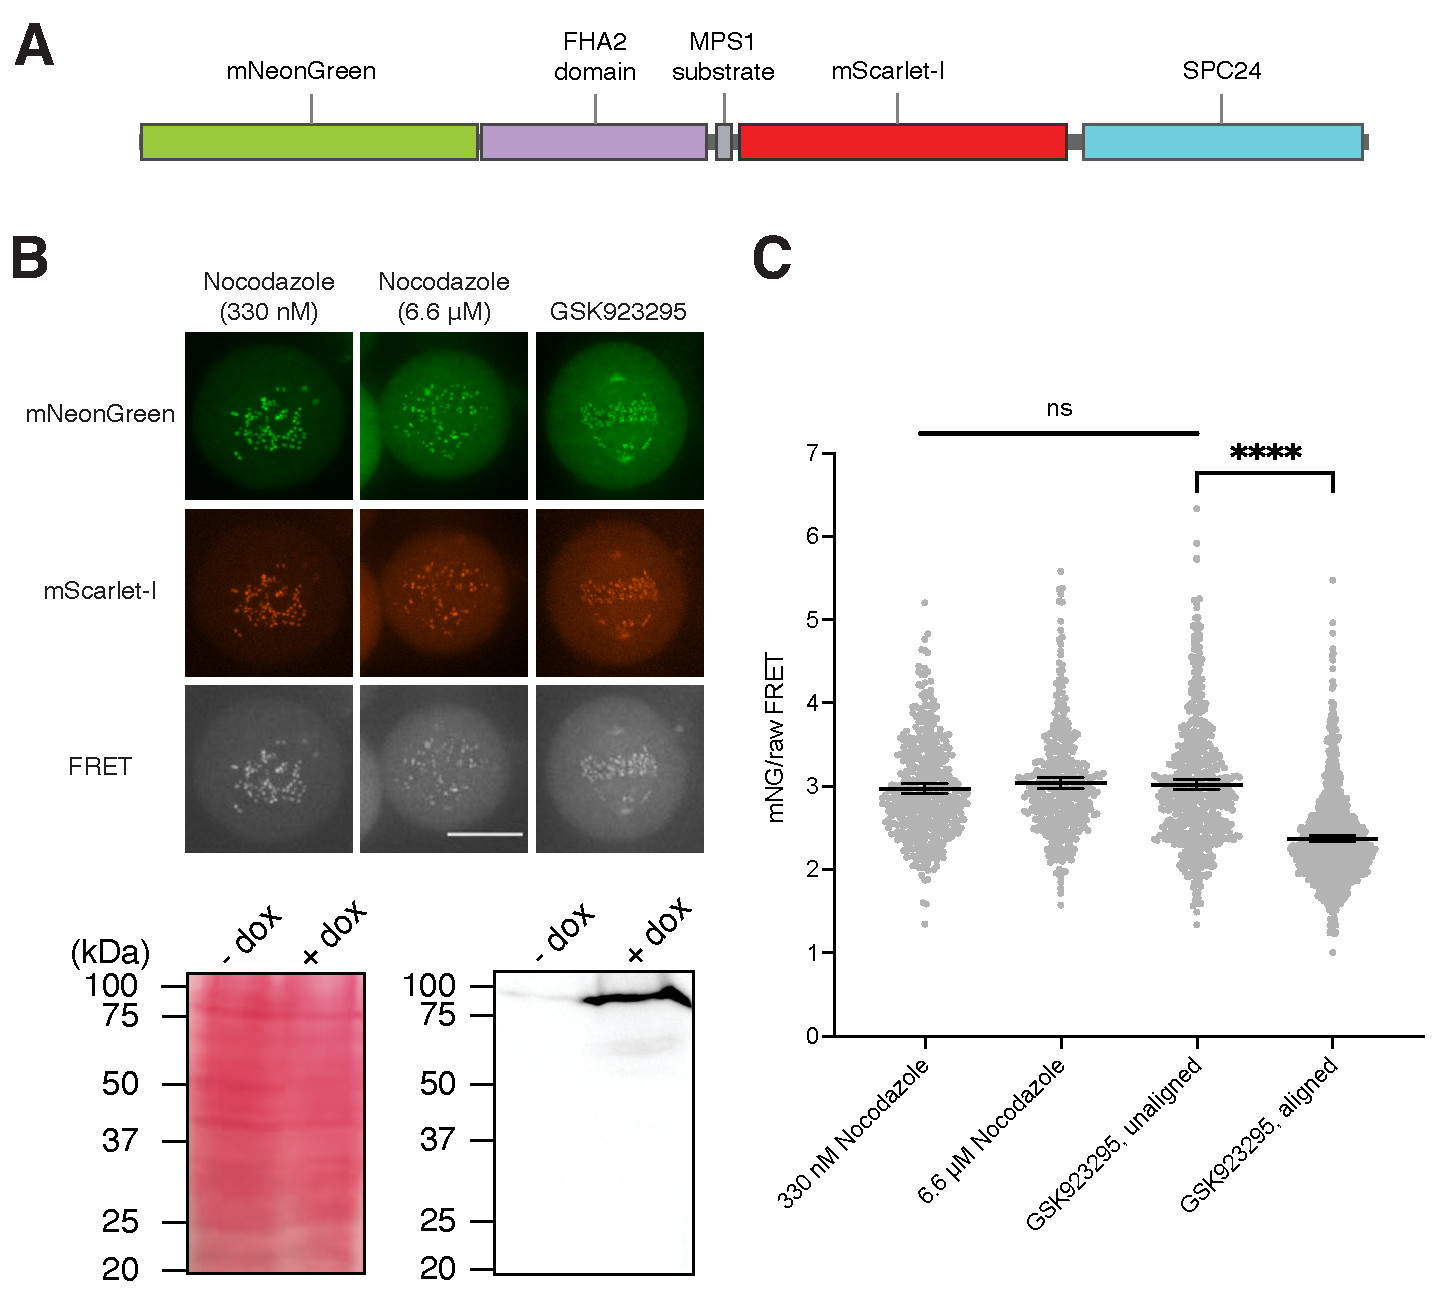
\includegraphics[width=\textwidth]{chapters/figures/MPS1sen-KT.pdf}
    \phantomsubfiglabel{MPS1sen-KT_Scheme} % subfigure A
    \phantomsubfiglabel{MPS1sen-KT_Images} % subfigure B
    \phantomsubfiglabel{MPS1sen-KT_FRETMetric} % subfigure C
    \caption{No difference in the \protein{Mps1}-phosphatases equilibrium at signaling kinetochores was detected in HeLa A12 when cells were treated with different drugs at various concentrations.}
    \label{MPS1sen-KT}
\end{figure}
\begin{figure}
    \noindent\justifying (Caption of \myref{MPS1sen-KT} continued from a previous page) (A) The design scheme of MPS1sen-KT. The \protein{Mps1} substrate sequence is \Peptide{LLEDGTLAINW}.
    The only difference between our version of the MPS1sen-KT and the original design \cite{MPS1senor} is that we used mNeonGreen/mScarlet-I as the acceptor/donor combination, which suits our confocal microscopy setup. (B) Top panel: representative confocal images of cells expressing MPS1sen-KT. MPS1sen-KT was recruited to both unaligned signaling kinetochores (in nocodazole- and GSK923295-treated cells) and non-signaling kinetochores aligned at metaphase plates (in GSK923295-treated cells) via its C-terminal \protein{Spc24} module. Brightness and contrast have been adjusted but the LUT for each channel (row) is universal for different groups (column). Scale bar, \SI{10}{\micro m}. Bottom panel: using an antibody against DsRed2 (which can detect many RFPs including mScarlet-I), we confirmed that MPS1sen-KT (with a theoretical molecular weight of \SI{97.2}{kDa}) can be induced by doxycycline to express as a full-length protein with negligible partial degradation or cleavage products in the RMCE HeLa-A12 cells (right blot). The Ponceau S staining of the same blot before blocking (left blot) served as the loading and transfer control. (C) A summary of a normalized FRET metric (mNeonGreen signal/FRET signal) in HeLa A12 cells treated with different drugs at various concentrations in (B). Each gray dot represents a single kinetochore measurement. Data were compiled from at least two independent experiments (with more than 40 cells and 400 kinetochores in each group). Mean values $\pm 95\%$ confidence intervals are overlaid. Data from cells treated with \SI{45}{nM}, \SI{90}{nM}, and \SI{200}{nM} GSK923295 were pooled together (they have no significant difference from one another) to simplify the presentation. Welch's analysis of variance (ANOVA) test [$W(\text{DF}n, \text{DF}d) = 1.339 (2.000, 917.0)$, $p = 0.2626$] was performed for the three columns on the left. The unpaired $t$-test with Welch's correction was performed to compare non-signaling kinetochores aligned at metaphase plates with unaligned signaling kinetochores in GSK923295-treated cells. Statistical tests are performed in Prism 9.
\end{figure}

We confirmed that MPS1sen-KT recruited to unaligned signaling kinetochores in both nocodazole- and GSK923295-treated cells had lower FRET efficiencies (higher \protein{Mps1}'s activity) compared to MPS1sen-KT recruited to non-signaling kinetochores aligned at metaphase plates in GSK923295-treated cells (\myref{MPS1sen-KT_FRETMetric}), consistent with the previous study \cite{MPS1senor}. However, in contrast to \cite{MPS1senor}, we did not observe any difference in \protein{Mps1}'s activity at unaligned signaling kinetochores in nocodazole- versus GSK923295-treated cells. This was irrespective of the concentrations of respective drugs and the reason for the conflicting observations may be cell line-specific. As far as the HeLa-A12 cell line is concerned, the difference in the numbers of SAC proteins recruited per signaling kinetochore in nocodazole- and GSK923295-treated cells should be mainly attributed to the difference in the total number of signaling kinetochores, which all compete for the limited pools of SAC proteins in the cell based on the law of mass action.

% It has been reported previously that the average localization levels of endogenously tagged HA-mCherry-\protein{Bub1} to signaling kinetochores in a CRISPR-Cas9-edited HeLa cell line treated with either \SI{250}{nM} of GSK923295 or \SI{6.6}{\micro M} of nocodazole were not significantly different \cite{MPS1senor}. One possible explanation is that the higher concentration of GSK923295 and the lack of filtering of cells based on the total number of unaligned chromosomes could mean more signaling kinetochores in GSK923295-treated cells.
% This observation contrasts with the previous report that the average localization levels of endogenously tagged HA-mCherry-Bub1 to signaling kinetochores in a CRISPR-Cas9-edited HeLa cell line treated with either 250 nM of GSK923295 or 6.6 μM of nocodazole were not significantly different (Kuijt et al., 2020). One possible explanation is that the much higher concentration of nocodazole in the aforementioned study may contribute to a more complete breakdown of spindles and a higher degree of phosphorylation of MELT motifs, while the lack of filtering of GSK923295-treated cells based on the number of unaligned chromosomes would lead to similar average numbers of signaling kinetochores in the nocodazole- and GSK923295-treated cells. We also cannot rule out the possibility that the differences reflect different Bub1 expression levels or kinase/phosphatase activities in the HeLa cell lines used.

\section{Recruitment of \protein{BubR1} by \protein{Bub1} \Latin{per se} contributes to the activity of the kinetochore-based SAC signaling}
\label{per_se}

% why BUBR1, instead of CDC20, BUB3, or MAD2?

Lastly, we sought to prove that the co-localization of multiple SAC proteins on the same \protein{Knl1} scaffold cooperatively boosts the kinetochore-based SAC signaling activity. Testing this non-linearity \Latin{in vivo} is currently beyond our capability considering the technical challenge to quantify the real-time signaling activity for each signaling kinetochore. As a compromise, we set out to examine whether enrichment of SAC proteins at kinetochores strengthens the SAC signaling activity.

Previous studies showed that \protein{BubR1} is mainly recruited to signaling kinetochores by heterodimerizing with \protein{Bub1} \cite{BubBiochem,BubR1TwoPools}. \protein{Bub1} is an important hub protein that binds to other SAC proteins (like \protein{Cdc20} and \protein{Mad1} which coordinately promote the formation of the \protein{Cdc20}-\protein{Mad2} heterodimer \Latin{in vitro} and in \Latin{Caenorhabditis elegans} \cite{BUB1-CDC20-MAD1,Tripartite}). We reasoned that \protein{BubR1}'s recruitment to signaling kinetochores by \protein{Bub1} may cause the local enrichment of \protein{BubR1} near where the \protein{Cdc20}-\protein{Mad2} dimer is formed and thereby facilitate the assembly of the MCC better than cytosolic free \protein{BubR1} does. Our eSAC activator-based mitotic duration assays (using truncations of \protein{Bub1} as the scaffold protein instead of the recombinant \protein{Knl1} phosphodomain in \myref{chpt:2}) showed that the recombinant \protein{Bub1} which can bind \protein{BubR1} promotes the SAC signaling activity better than the recombinant \protein{Bub1} which is unable to bind \protein{BubR1} does (manuscript in preparation). However, a previous study showed that % the deletion of the heterodimerization domain of \protein{Bub1} (in an in vitro assay \cite{BUB1-CDC20-MAD1}) or
abolishing the heterodimerization between \protein{BubR1} and a recombinant, kinetochore-tethered \protein{Bub1} did not affect the SAC signaling activity \cite{MIS12-BUB1-E252K}. Moreover, two previous \protein{BubR1} knockdown-rescue experiments in nocodazole-treated cells published by different research groups demonstrated that \protein{BubR1}'s recruitment to signaling kinetochores by \protein{Bub1} counter-intuitively shortens the duration of the mitotic arrest \cite{BubR1TwoPools,BubBiochem}. Even though the two studies deleted different segments of \protein{BubR1}'s heterodimerization domain which mediates \protein{BubR1}'s interaction with \protein{Bub1} (a.a 440-460 \cite{BubR1TwoPools}, henceforth referred to as ``HD\textsuperscript{short}'', versus a.a. \textDelta{}432-484 \cite{BubBiochem}, henceforth referred to as ``HD'') and used different concentrations (\SI{\sim100}{nM} in \cite{BubR1TwoPools} versus \SI{50}{nM} in \cite{BubBiochem}) of nocodazole to induce signaling kinetochores, their basic observations were nonetheless consistent. We also did a similar knockdown-rescue experiment in GSK923295-treated cells comparing the SAC signaling activity of wildtype \protein{BubR1} and \protein{BubR1}(\textDelta{}HD\textsuperscript{short}), whose results were also consistent with these two studies (\myref{OldBUBR1Rescue}). These conflicting pieces of evidence inspired us to examine the matter more carefully.
% which might have resulted in the observation of different levels of heterodimerization domain-truncated \protein{BubR1} remaining at signaling kinetochores.

We noted that first, there lacked rigorous control over the expression level of the ectopic recombinant \protein{BubR1} to match the physiological expression of endogenous \protein{BubR1} in the knockdown-rescue experiments in \cite{BubBiochem, BubR1TwoPools}.

Second, the concentrations of nocodazole used in these two studies allowed the existence of some spindle microtubules \cite{RZZ-MAD1vsBUB1-MAD1_2015}. However, PP2A's recruitment by \protein{BubR1}'s kinetochore attachment regulatory domain (KARD) to signaling kinetochores is known to contribute to the silencing of the SAC either directly (by dephosphorylating the MELT motif \cite{PP2ADephosphorylatesKNL1} or \protein{Bub1} \cite{PP2ADephosphorylatesBUB1}) or indirectly (by stabilizing the kinetochore-microtubule attachment \cite{BUBR1_KT-MT, Suijkerbuijk2012, BUBR1-L669A+I672A, PP2A-B56-BUBR1ChromosomeCongression_Xu2013} or promoting PP1's recruitment \cite{PP2A-B56}). PP2A's recruitment to signaling kinetochores might not be completely canceled by \protein{BubR1}(\textDelta{}HD)'s defective interaction with B56 \cite{BubBiochem}, knock-down of B56's (due to probable incomplete knock-down), or KARD mutations (\cite{BubR1TwoPools}, which eliminated the binding of the B56\textalpha{} isoform \cite{BUBR1-L669A+I672A}). The dual functions of \protein{BubR1} (participating in the assembly of the MCC as well as promoting the recruitment of PP2A) converge on promoting accurate chromosome segregation during normal mitosis, but their entanglement complicates the validation of the role of \protein{BubR1}'s localization to signaling kinetochores in the SAC signaling activity.

Third, although the depletion of \protein{BubR1} does not affect the localization of \protein{Cenp-E} at signaling kinetochores in HeLa cells \cite{CENPELocalization-BUBR1}, the activity of kinetochore-localized \protein{Cenp-E} (to facilitate the transition of the kinetochore-microtubule attachment from lateral to end-on) is arguably affected by the loss of interaction with \protein{BubR1} \cite{CENPEActivity-BUBR1} when cells are rescued by heterodimerization domain-truncated \protein{BubR1}, which may thereby affect chromosome congression. % CENP-E binds to PP1 and Aurora kinases can dynamically regulate this interaction to promote chromosome alignment (Kim et al., 2010). 

Therefore, we designed and performed a new \protein{BubR1} knockdown-rescue experiment. Here, the SAC signaling activity of \protein{BubR1}(\textDelta{}KARD) and \protein{BubR1}(\textDelta{}KARD, \textDelta{}HD) was compared (\myref{RecombinantBUBR1Diagram}). The truncation of KARD (a.a. 665-682) abolishes the binding of B56\textalpha{} \cite{Suijkerbuijk2012} and likely other isoforms of B56 onto \protein{BubR1} as well \cite{B56-SLiM, PP2A-B56-BUBR1Structure}, which allow us to dissect whether the recruitment of \protein{BubR1} to the signaling kinetochore \Latin{per se} contributes to the SAC activity. Additionally, mNG-\protein{BubR1}(\textDelta{}HD, \textDelta{}KARD) lacks the heterodimerization domain (HD). We imaged our genome-edited mNG-\gene{BubR1} HeLa-A12 cell line (treated with the AllStars negative control siRNA) at the same time to serve as a reference for the endogenous expression of \protein{BubR1} (first column, \myref{NewBUBR1Rescue}). Only mitotic cells having $0.5\times$ -- $2\times$ the average mNeonGreen intensity of mNG-\gene{BubR1} HeLa-A12 cells during mitosis were included in the analysis (noted that only about half of endogenous \protein{BubR1} proteins are tagged in the CRISPR-Cas9-edited cell line).

Just like what was shown in \cite{BubBiochem}, mNG-\protein{BubR1}(\textDelta{}HD, \textDelta{}KARD) had minimal localization at signaling kinetochores  (\myref{BUBR1del432-484KTLocalization}). The mitotic arrest was induced by treatment with \SI{25}{nM} of nocodazole \cite{25nMNoc} after thymidine release, where unattached kinetochores can be observed while metaphase plates remain largely intact (\myref{BUBR1del432-484KTLocalization}).

\begin{figure}
    \centering
    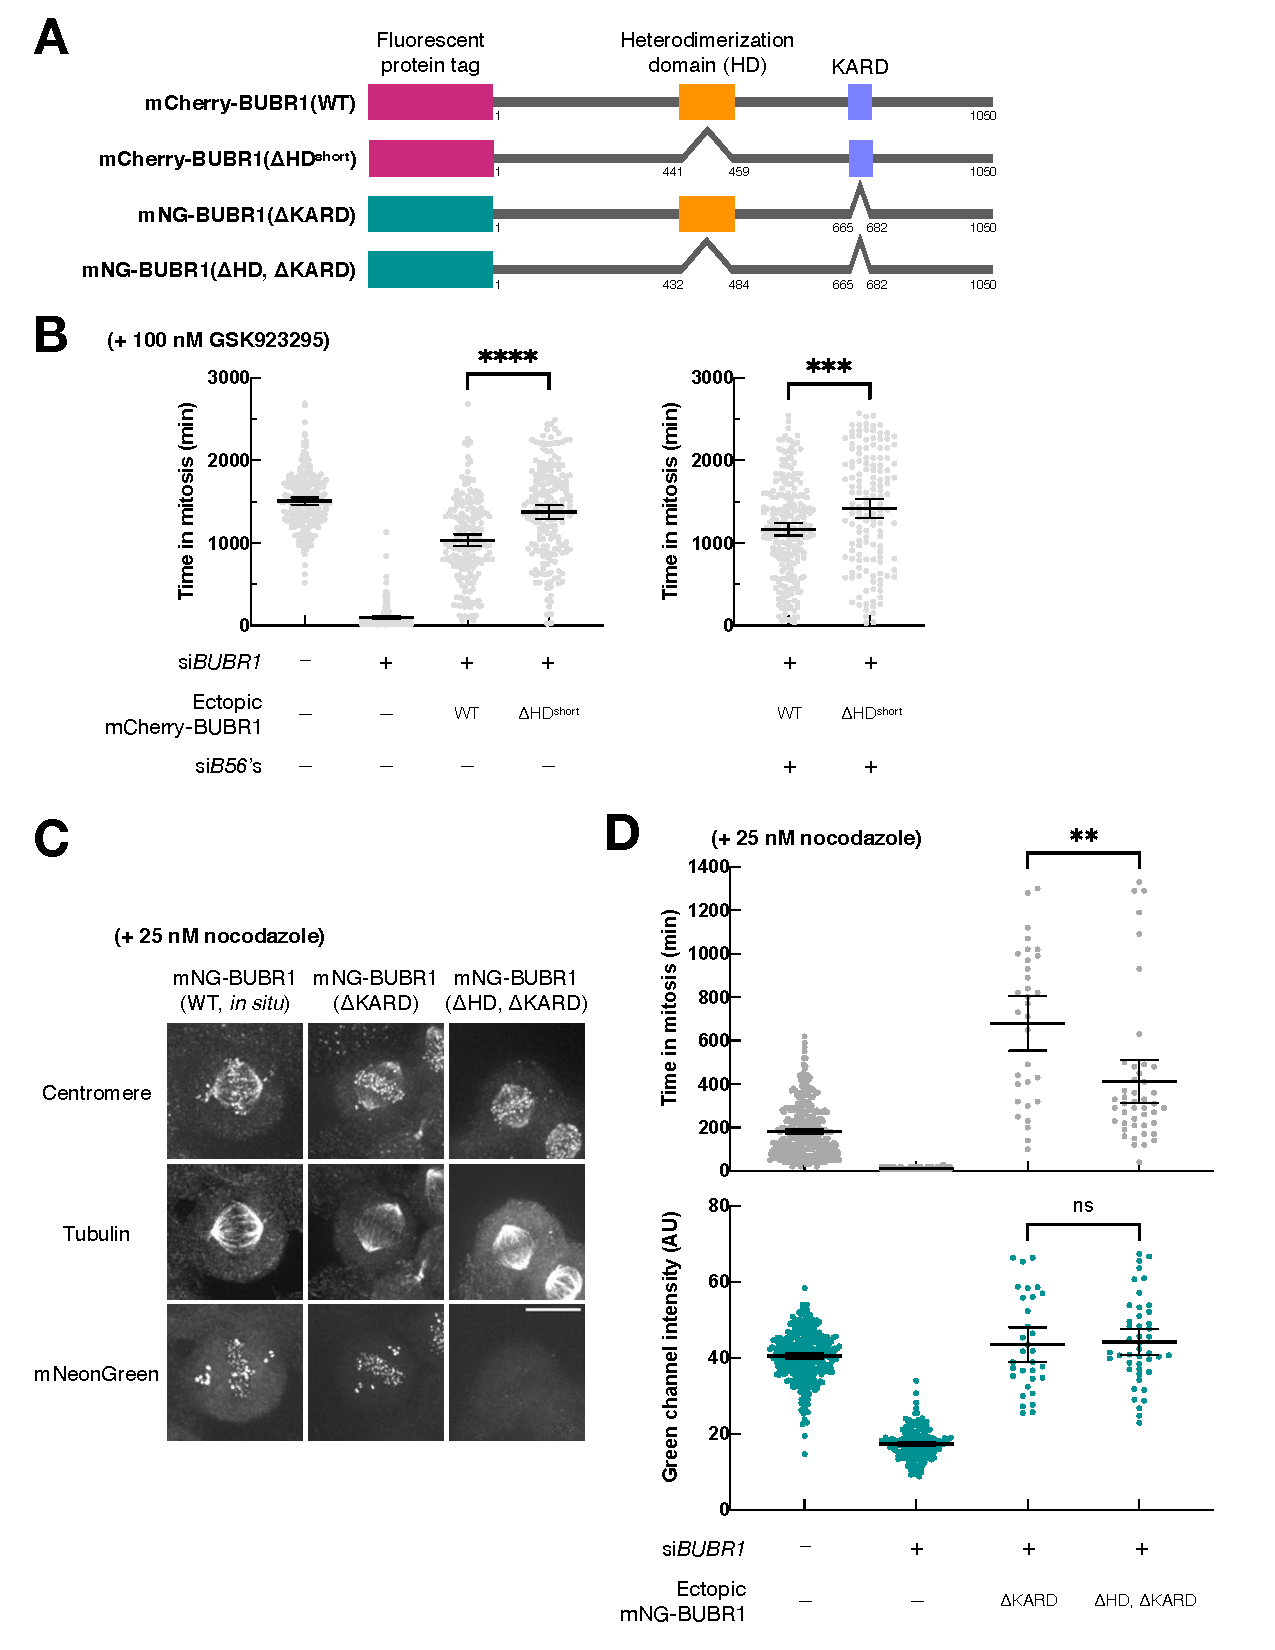
\includegraphics[width=0.99\textwidth]{chapters/figures/RescueExperiment.pdf}
    \phantomsubfiglabel{RecombinantBUBR1Diagram} % subfigure A
    \phantomsubfiglabel{OldBUBR1Rescue} % subfigure B
    \phantomsubfiglabel{BUBR1del432-484KTLocalization} % subfigure C
    \phantomsubfiglabel{NewBUBR1Rescue} % subfigure D
    \caption{Recruitment of \protein{BubR1} by \protein{Bub1} to signaling kinetochores \Latin{per se} contributes to the SAC signaling activity.}
    \label{RescueExperiment}
\end{figure}
\begin{figure}
  \noindent\justifying (Caption of \myref{RescueExperiment} continued from a previous page) (A) Diagrams (not to scale) of all ectopic recombinant BUBR1's used in experiments associated with \myref{OldBUBR1Rescue,BUBR1del432-484KTLocalization,NewBUBR1Rescue}. (B) A \gene{BubR1} knockdown-rescue experiment with mCherry-\protein{BubR1} or mCherry-\protein{BubR1}(\textDelta{}HD\textsuperscript{short}) (with an HD truncation from \cite{BubR1TwoPools}). \cite{BubR1TwoPools} uses a shorter HD truncation compared to \cite{BubBiochem}. Therefore, it is denoted as \textDelta{}HD\textsuperscript{short} here. We used \SI{100}{nM} GSK923295 to activate the SAC, which is different from both \cite{BubR1TwoPools} (\SI{100}{nM} nocodazole) and \cite{BubBiochem} (\SI{50}{nM} nocodazole). Cells rescued with mCherry-\protein{BubR1} consistently have a lower SAC signaling activity than cells rescued with mCherry-\protein{BubR1}(\textDelta{}HD\textsuperscript{short}), no matter whether B56's were knocked down. Cells treated with si\gene{BubR1} and rescued with mCherry-\protein{BubR1} had a lower SAC signaling activity than the host cell line treated with the AllStars negative control siRNA, probably due to the lack of control over the expression of the ectopic mCherry-\protein{BubR1}. Each dot represents a cell, with more than 140 cells in each group. The mean value $\pm$ the 95\% confidence interval of each group is overlaid. Unpaired $t$-tests with Welch's correction are performed in Prism 9. Frank Ferrari also contributed to the data analysis here. (C) Confocal immunofluorescence micrographs (by Dr. Ajit Joglekar) showed that \SI{25}{nM} nocodazole impaired the congression of a few chromosomes (which activated the SAC) in both genome-edited mNG-\gene{BubR1} HeLa-A12 cells (the first column) and the RMCE HeLa-A12 cells (the second and the third columns). In the second and the third columns, the RMCE HeLa-A12 cells were treated with si\gene{BubR1} and \SI{0.5}{\micro g/mL} of doxycycline to induce the ectopic expression of indicated mN-\protein{BubR1} variants. Ectopically expressed mNG-\protein{BubR1}(\textDelta{}HD, \textDelta{}KARD) could not be detected at kinetochores (the third columns). Maximum $z$-projections of representative cells were shown for each condition (column) and channel (row). The LUTs for the mNeonGreen channel are the same across different conditions. Scale bar, \SI{10}{\micro m}. (D) A \gene{BubR1} knockdown-rescue experiment with mNG-\protein{BubR1}(\textDelta{KARD}) or mNG-\protein{BubR1}(\textDelta{}HD, \textDelta{}KARD) (with an HD truncation from \cite{BubBiochem}). Top panel: the duration of mitosis of individual cells treated with \SI{25}{nM} nocodazole. Bottom panel: the average cytosolic mNeonGreen signal from the same cells right after the NEBD. In the heterozygous, genome-edited mNG-\gene{BubR1} HeLa-A12 cells (first two columns), both the wildtype allele and the edited mNG-\gene{BubR1} allele are susceptible to si\gene{BubR1}. In the RMCE HeLa-A12 cells (last two columns), ectopically expressed mN-\protein{BubR1} variants are resistant to si\gene{BubR1}. Each dot represents a cell, with more than 30 cells in each group. Results are representative of two independent experiments. The mean value $\pm$ the 95\% confidence interval of each group is overlaid. Unpaired $t$-tests with Welch's correction are performed in Prism 9.
\end{figure}

Our knockdown of \gene{BubR1} was sufficient to almost completely abolish the SAC signaling activity (first two columns, \myref{NewBUBR1Rescue}). mNG-\protein{BubR1}(\textDelta{}KARD)-rescued cells take longer in mitosis than the control group (the third column versus the first column, \myref{NewBUBR1Rescue}), which is consistent with previous studies \cite{PP2A-B56, BUBR1-L669A+I672A}. Most importantly, our new data showed that mNG-\protein{BubR1}(\textDelta{}KARD)-rescued cells had a higher SAC signaling activity than mNG-\protein{BubR1}(\textDelta{}HD, \textDelta{}KARD)-rescued cells did (\myref{NewBUBR1Rescue}), directly supporting that the recruitment of \protein{BubR1} \Latin{per se} contributes to the activity of the kinetochore-based SAC signaling.

\section{Discussion}
\label{Chapter3Discussions}

In this chapter, we demonstrated that the competition among a large number of signaling kinetochores can effectively diminish freely diffusive SAC proteins in the cytosol. This, instead of a potential shift in the degree of phosphorylation of MELT motifs, presumably explains why the numbers of SAC proteins recruited per signaling kinetochore are inversely correlated with the total number of signaling kinetochores in the cell. Using the recruitment of \protein{BubR1} by \protein{Bub1} as an example, we showed that the co-localization of multiple SAC proteins on the same \protein{Knl1} scaffold likely strengthens the SAC signaling activity. Even though we did not rigorously prove that the cooperative signaling among multiple SAC proteins on the same \protein{Knl1} scaffold boosts the kinetochore-based SAC signaling activity non-linearly, all data presented in this chapter supported the model in \myref{ProzoneEffectModel}.

By knocking down \gene{ZW10}, we dissected the contribution of the core SAC pathway to the kinetochore localization of SAC proteins. However, it should be noted that \protein{Mad1} may also be recruited to signaling kinetochores by the kinetochore protein \protein{Cep57} \cite{MIS12-CEP57-MAD1-MAD2}. Further studies are needed to clarify whether the \protein{Cep57} pathway, the corona pathway, and the \protein{Knl1}-\protein{Bub1} (core SAC) pathway of \protein{Mad1} recruitment work cooperatively.

The dynamic and stochastic establishment of kinetochore-microtubule attachment influences the localization of SAC protein and the dynein-dependent stripping of the corona \cite{SACSilencing_Etemad2019, SACSilencing_Kuhn2019, CENP-FLimitsStripping}. We envision that right after the NEBD, all signaling kinetochores in a human cell are fully unattached. As the cell progress normally through the prometaphase, kinetochores gradually and independently establish end-on attachment to spindle microtubules. When we take a snapshot of a human cell near the end of the prometaphase, instead of one completely unattached kinetochores and 91 fully attached kinetochores that have already completely silenced their local SAC signaling activity, there may be three minimally attached kinetochores and 89 mostly attached kinetochores that are still in the process of stripping the corona and silencing the local SAC signaling activity. It remains to be seen whether (or how) the idea of dynamic regulation of the SAC signaling activity per kinetochore based on the total number of signaling kinetochores applies to this physiological scenario.

% The potentially reduced \protein{Cenp-E} activity at the kinetochore in mNG-\protein{BubR1}(\textDelta{}HD, \textDelta{}KARD)-rescued cells should only result in an increased SAC response, compared to mNG-\protein{BubR1}(\textDelta{}KARD)-rescued cells.
\protein{BubR1} interacts with the kinase \protein{Plk1}, a key regulator throughout mitosis \cite{BUBR1-PLK1}. mNG-\protein{BubR1}(\textDelta{}KARD) may still recruit \protein{Plk1} to signaling kinetochores, while mNG-\protein{BubR1}(\textDelta{}HD, \textDelta{}KARD) (which itself minimally localized to signaling kinetochores) can not. Although depletion of \protein{BubR1} only results in a marginal reduction of \protein{Plk1} at signaling kinetochores \cite{CENPU+BUB1-PLK1}, it remains to be examined how much the discrepancy in the localization of \protein{Plk1} contributes to the SAC signaling activity in the knockdown-rescue experiment of \protein{BubR1}.

In our manuscript, Soubhagyalaxmi Jema further showed that an increased expression of \protein{Bub1} enhanced the recruitment of \protein{BubR1} to signaling kinetochores and the SAC signaling activity. These observations demonstrated that the SAC signaling activity is partially limited by the low expression level of \protein{Bub1} in HeLa-A12 cells. We hypothesized that this could be the result of a compromise among various sources of selection pressure. Like \protein{BubR1}, whose recruitment to signaling kinetochores improves the SAC signaling activity and promotes chromosome congression, \protein{Bub1} also has multiple functions (for example, in telomere replication \cite{BUB3-BUB1_TelomereReplication}, \protein{Plk1}'s localization \cite{CENPU+BUB1-PLK1}, and the correction of erroneous kinetochore-microtubule attachment \cite{BUB1_pH2A_AuroraB}). The MCC is even involved in the clathrin-mediated endocytosis of insulin receptors \cite{MCC_IREndocytosis, Choi2019}. How these functions of SAC proteins interact and integrate is a fascinating topic that may lead to exciting discoveries. % (for example, between the sensitivity of the SAC to detect a small number of unattached kinetochores and the responsiveness of the SAC to silence once all chromosomes establish proper bipolar attachment and are aligned at the metaphase plate \cite{eSAC})

\section{Materials and methods}
For methods of cell culture and Cre-\bacterialgene{lox} RMCE, see \myref{CellCulture+RMCE_Methods}.

\subsection{CRISPR-Cas9-mediated genome editing}
\label{CRISPRMethods}
The guide RNAs (gRNAs) for \Latin{in situ} \gene{BubR1} and \gene{Bub1} N-terminal mNeonGreen-tagging were \Oligo{caggauggcggcggugaaga} and \Oligo{gguucagguuuggccgcugc},
%#9 \Oligo{gguucagguuuggccgcugc}
respectively. The gRNA for \Latin{in situ} \gene{Mad1} C-terminal mNeonGreen-tagging was \Oligo{cagaccguggcguagccugc}. Single guide RNAs (sgRNAs) were synthesized using the EnGen sgRNA Synthesis Kit (for the \Latin{Streptococcus pyogenes}-originated Cas9, New England Biolabs). The \Latin{Sp}Cas9-sgRNA ribonucleoprotein (RNP) complex was assembled at room temperature in a buffer consisting of \SI{20}{mM} of HEPES-KOH (pH 7.5), \SI{150}{mM} of KCl, \SI{1}{mM} of MgCl$_2$, 10\% (by volume) of glycerol, and \SI{1}{mM} of DTT using \SI{100}{pmol} of \Latin{Sp}Cas9-$2\times$NLS (the QB3 MacroLab) and \SI{120}{pmol} of sgRNA. The RNP complex and \SI{1.5}{\micro g} of the corresponding linearized homology-directed repair template plasmid were co-transfected into $2\times 10^5$ -- $5\times 10^5$ nocodazole-arrested mitotic HeLa-A12 cells \cite{CRISPRProtocol} (harvested by the mitotic shake-off method) using the Cell Line Nucleofector\texttrademark{} Kit R (Lonza) following the manufacturer's instructions. After one week, green fluorescence-positive mitotic cells (arrested by \SI{330}{nM} nocodazole for \SI{16}{h}) were sorted directly into 96-well plates at one cell per well. Healthy colonies were subject to further validation by fluorescence imaging, genotyping (and subsequent sequencing), as well as immunoblotting.

Successfully edited alleles encode mNeonGreen-tagged SAC proteins wherein the corresponding wildtype protein and mNeonGreen are separated by a short flexible linker (mNG-\protein{BubR1} and mNG-\protein{Bub1}: \Peptide{GSGGSG}; \protein{Mad1}-mNG: \Peptide{GGAGGSGG}).

\subsection{Genotyping}
HeLa-A12 genomic DNAs were purified using the Wizard\textsuperscript{\textregistered} SV Genomic DNA Purification System (Promega). Genotyping primers (\gene{BubR1} forward primer \Oligo{cctggtcacatctgagctat},
% cctggtcacatctgagctat 1942 ?
\gene{BubR1} reverse primer \Oligo{ctcagtgagactccagtgtt},
% ctcagtgagactccagtgtt 1943 ?
\gene{Bub1} forward primer \Oligo{ccctctacatgaaggcgcta},
% ccctctacatgaaggcgcta 2082 ? 
\gene{Bub1} reverse primer \Oligo{gctcgcccaaggtaaacatt},
% gctcgcccaaggtaaacatt 2083 ?
\gene{Mad1} forward primer \Oligo{ GGACTTTTCAGGGACGTGGT},
% GGACTTTTCAGGGACGTGGT 2094 ?
and \gene{Mad1} reverse primer \Oligo{GAGTTGGGAGGAGGGGACTC})
% GAGTTGGGAGGAGGGGACTC 2093 ?
were designed to bind outside of homology arms to avoid false-positive colonies from integration of the homology-directed repair template plasmid to an off-target genomic locus. Genotyping PCR products were qualitatively analyzed by 1\% agarose-TAE gel stained by ethidium bromide and individual bands were subsequently submitted for Sanger sequencing.

\subsection{Rapid amplification of cDNA ends (RACE)}
Interphase samples were arrested in \SI{2.5}{mM} of thymidine for one day and then harvested by trypsinization. Mitotic samples were arrested in \SI{2.5}{mM} of thymidine for one day, released into \SI{100}{ng/mL} of nocodazole for \SI{19}{h}, and finally harvested by mitotic shake-off. Harvested cells were snap-frozen by liquid nitrogen and stored at \SI{-80}{\celsius} until total RNA extraction.

Total RNA extraction was done using the Monarch Total RNA Miniprep Kit (New England Biolabs) following the manufacturer’s instructions. The reverse transcription (RT) was done using the Template Switching RT Enzyme Mix (New England Biolabs) following the manufacturer’s instructions. The sequence of the template-switching oligo is \MixedOligo{GCTAATCATTGCAAGCAGTGGTATCAACGCAGAGTACATrGrGrG}. The sequence of the \gene{Bub1}-specific RT reverse primer (which binds to the fourth exon of \gene{Bub1}) is \Oligo{ctctgaaggacagcactggcat}.

The reverse transcription products were subsequently amplified by nested PCR. The template-switching oligo-specific forward primer (incorporating a \textit{Spe}I restriction site at the 5' end) is \Oligo{GGACTAGTTGCAAGCAGTGGTATCaac}. The \gene{Bub1}-specific reverse primer (incorporating an \textit{Xho}I restriction site at the 3' end) is \Oligo{TATACTCGAGctctccttgggcttccagat}, which binds to the fourth exon of \gene{Bub1} as well but upstream of the RT reverse primer.

RT-PCR products were visualized on an agarose gel. Individual bands were cut off and purified from the gel, and finally cloned into pBlueScript-KS(+) between the \textit{Spe}I site and the \textit{Xho}I site. For each band, multiple clones were randomly picked for sequencing.

\subsection{Fluorescence correlation spectroscopy (FCS)}
\label{FCSMethods}

The total number of fluorophores in a homogeneous solution is $N_\text{total} := N_\text{A}cV_\text{total}$, where $N_\text{A}$ is the Avogadro constant, $c$ is the molar concentration of the fluorophore, and $V_\text{total}$ is the total volume of the solution. The probability that a specific fluorophore molecule is within the excitation volume $V_0 (\ll V_\text{total})$ at any given time is $p_0 := V_0/V_\text{total}\ll1$. For freely diffusive fluorophores in a diluted solution, whether or not a specific fluorophore is within the excitation volume is independent of each other. Thus, the number of fluorophores inside the excitation volume at any given time $N_0$ has a binomial distribution $B(N_\text{total}, p_0)$. Therefore, the auto-correlation at 0-time lag
\begin{equation*}
    G_0 \coloneqq \dfrac{\sigma_{N_0}^2}{\langle N_0 \rangle^2} = \dfrac{1-p_0}{N_\text{total}p_0} \approx \dfrac{1}{N_\text{A}cV_0}.
\end{equation*}
Under a fixed live-cell imaging setup [which includes the microscope (its alignment and the objective), the wavelength of the excitation light, the thickness of the coverslip (affecting the actual working distance), and the refractive index of the cytosol], $V_0$ is fixed. Therefore, $G_0$ is inversely proportional to the molar concentration of the fluorophore. The average number (or the variance of the number) of fluorophores inside the excitation volume observed over a long period should be close to the theoretical mean $\langle N_0 \rangle$ (or the theoretical variance $\sigma_{N_0}^2$).

All FCS data were collected on an Alba v5 Laser Scanning Microscope (ISS), connected to an Olympus IX81 inverted microscope main body [equipped with a UPLSAPO60XW objective (1.2 NA, Olympus)]. A Fianium WL-SC-400-8 laser (NKT Photonics) with an acousto-optic tunable filter was used to generate excitation pulses at a wavelength of \SI{488}{nm} and a frequency of about \SI{20}{MHz}. Excitation light was further filtered by a Z405/488/561/635rpc quadband dichroic mirror (Chroma). Emission went through a 655DCSPXR short-pass dichroic mirror (Chroma) and an FF01-531/40-25 filter (Semrock) and was finally detected by an SPCM-AQRH-15 avalanche photodiode (Perkin Elmer). The time-correlated single photon counting module to register detected photon events to excitation pulses was SPC-830 (Becker \& Hickl). Data acquisition was facilitated by VistaVision (ISS). The excitation volume ($V_0$) was calibrated by taking FCS data from TetraSpeck\texttrademark{} microspheres (\SI{0.1}{\micro m}, Invitrogen) of known concentrations (vary across different batches).

\subsection{RNA interference (RNAi)}

Cells were transfected with siRNA in the morning. \SI{2.5}{mM} of thymidine was added \SI{8}{h} later and cells were incubated overnight. The next morning, cells were released from the thymidine block into fresh media. This sequence was then repeated once again and cells were released into FluoroBrite\texttrademark{} DMEM supplemented with 9\% (by volume) of fetal bovine serum and $1\times$ GlutaMAX and incubated for \SI{6}{h} before the addition of mitotic drugs. Imaging was started at least \SI{1}{h} after drug treatment.

Sense-strand sequences and working concentrations of small interfering RNA duplexes (siRNAs) used in this study include the \gene{BubR1} siRNA (\Oligo{GAUGGUGAAUUGUGGAAUA}, \SI{40}{nM} \cite{BubR1MitosisTurnover}), \gene{Bub1} siRNA (\Oligo{CGAAGAGUGAUCACGAUUU}, \SI{40}{nM} \cite{BUB1-si5}), and the \gene{ZW10} siRNA (\Oligo{UGAUCAAUGUGCUGUUCAA}, \SI{100}{nM} \cite{BUBR1_XenopusVSHeLa}). The siRNAs against all five B56 isoforms were taken from the second pool in \cite{siB56s}.
%the \gene{Knl1} siRNA (\Oligo{CACCCAGUGUCAUACAGCCAAUAUU},
%       CACCCAGUGUCAUACAGCCAAUAUU HSS183683
%40 nM \cite{KI2014}).
Desalted siRNAs modified by double-deoxythymidine overhangs at 3'-ends of both strands were synthesized by Sigma. The AllStars Negative Control siRNA (QIAGEN) was used as the control. All siRNAs were transfected into the cells via Lipofectamine RNAiMAX (Invitrogen) following the manufacturer’s instructions.

\subsection{Live-cell imaging}
\label{chpt3ImagingMethods}

Cells were plated in a Nunc Lab-Tek II chambered coverglass (Thermo Scientific) or a 35-mm coverglass-bottomed dish (MatTek) and treated with drugs and/or siRNAs accordingly. For imaging, the chambered coverglass or the coverglass-bottomed dish was loaded into a CU-501 temperature and gas control system (Live Cell Instrument). The sample holder was maintained at \SI{37}{\celsius} and ventilated by humidified 5\% of \ch{CO2} and the objective was maintained at \SI{37}{\celsius} by a heating band.

Most wide-field, $z$-stack fluorescence imaging (except the measurement of FRET efficiency of MPS1sen-KT) was performed on a Nikon Eclipse Ti-E/B inverted microscope, with a CFI Plan Apochromat Lambda $100\times$, 1.45 NA oil objective (Nikon). The intermediate magnification selector knob was switched to $1\times$ unless specified otherwise. The microscope was equipped with an H117E1 motorized stage (Prior Scientific) and a NanoScanZ 100 piezo stage (Prior Scientific). A SPECTRA 5-LCR-XA Light Engine (Lumencor) served as the excitation light source. The 475 nm-centered band of excitation light was used for the green channel and the 575/30-nm-filtered band of excitation light was used for the red channel. An ET-EGFP/mCherry filter cube (Chroma Technology) was used as the dichroic mirror, where the built-in emission filter on the cube has been removed. Emission light in the red channel was filtered by an ET632/60m (Chroma Technology). Emission light in the green channel was filtered by an ET525/50m (Chroma Technology). Emission filters were mounted on a high-speed filter wheel (Prior Scientific) positioned in the light path before the iXon3 EMCCD camera (Andor Technology) operating in the conventional CCD mode. Signaling kinetochores in GSK923295-treated cells were identified by their polar positioning and the enrichment of localized SAC proteins on them. Custom MATLAB programs \cite{HeLaFRETGUI} were used to quantify kinetochore-localized fluorescence signals.

The FRET measurement with MPS1sen-KT was also performed on a Nikon Eclipse Ti-E/B inverted microscope, with a CFI Plan Apochromat VC $100\times$, 1.40 NA oil objective (Nikon). The intermediate magnification selector knob was switched to $1\times$. The microscope was equipped with an H117E1 motorized stage, a NanoScanZ 100 piezo stage, and an X-Light V2 L-FOV confocal unit with \SI{60}{\micro m} pinholes (CrestOptics). A CELESTA Light Engine (Lumencor) served as the excitation laser source. The 477-nm line (at $25\%$ power with an exposure time of \SI{400}{ms} for each frame) was used for both the green and the FRET channels and the 546-nm line (at $50\%$ power with an exposure time of \SI{400}{ms} for each frame) was used for the red channel. A ZT488/543rpc (Chroma Technology) was used as the dichroic mirror. Emission through both the red and the FRET channels was filtered by an ET605/52m (Chroma Technology) while emission through the green channel was filtered by an ET525/36m (Chroma Technology). Images were acquired by a Prime 95B 25mm sCMOS camera (Teledyne Photometrics). Custom MATLAB programs \cite{HeLaFRETGUI} were used to quantify kinetochore-localized fluorescence signals.

Time-lapse live-cell imaging related to the knockdown-rescue experiments was performed on an ImageXpress Nano Automated Imaging System (Molecular Devices). A SOLA Light Engine (Lumencor) served as the excitation light source. Cells were plated on 24-well cell imaging plates (black plate with treated glass bottom, Eppendorf) and treated with drugs and/or siRNAs accordingly. Input humidified $5\%$ \ch{CO2} flow was maintained at around \SI{19}{psi} and the environment chamber was maintained at \SI{37}{\celsius}.

All SAC proteins tagged by mNeonGreen in this chapter (\protein{BubR1}, \protein{Bub1}, and \protein{Mad1}) feature inhomogeneous distributions between the cytosol and the nucleus/nuclear envelope in the prophase (data not shown). In principle, they can indicate the accurate timing of the nuclear envelope breakdown (NEBD) in each cell during the time-lapse imaging. However, due to the resolution limit and for consistency, we determined mitotic duration mainly based on cell morphology (from rounding-up at the NEBD to elongation at the anaphase onset) from transmitted-light images. This was facilitated by the semi-automatic image analysis pipeline described in \myref{IncuCyteAnalysis}. % Unless specified otherwise

\subsection{Quantification of the FRET efficiency by kinetochore-localized fluorescence signals of MPS1sen-KT}
\label{FRETMetricTheory}

Under fixed fluorescence microscopy settings of a given channel [the excitation line and its power, exposure time, optical components (including the objective, filters, dichroic mirrors, the confocal spinning disk, and the detector) in the light path and their alignment, etc.], the kinetochore-localized fluorescence signal (digital readout) should be proportional to the number of localized mature fluorescence proteins. The coefficients are designated as $g$ and $r_x$ for mNeonGreen and mScarlet-I using the excitation light for mNeonGreen, respectively (the subscript ``x'' stands for cross-excitation 
as mScarlet-I is excited by the excitation light for mNeonGreen here). The number of unbleached mature mNeonGreen and mScarlet-I molecules at a given kinetochore are $G$ and $R$, respectively. While measuring FRET using the excitation light for mNeonGreen and optics settings to detect the emission of mScarlet-I, the bleed-through coefficient of mNeonGreen's fluorescence is designated as $\beta$. Under a FRET efficiency of $\varepsilon$ $(0 \leq \varepsilon \leq 1,$ which describes the quenching of mNeonGreen due to FRET), the proximity ratio $\Theta$, a metric of FRET according to the definition in \cite{HeLaFRETGUI}, can be expressed as
\begin{equation*}
    \Theta := \dfrac{F}{r_xR + \beta gG(1 - \varepsilon)} - 1,
\end{equation*}
where $F$ is the measured raw FRET readout. $F$ can be attributed to three sources: (1) the cross-excitation of mScarlet-I, (2) the bleed-through of mNeonGreen's fluorescence, and (3) the actual fluorescence due to FRET (determined by the combined coefficient $f$ for the excited fraction of mNeonGreen under the excitation condition of the FRET channel and the conversion from FRET emission photons reaching the detector to the digital readout, the FRET efficiency $\varepsilon$, and the effective quantum yield $\phi$ of mScarlet-I that reaches the detector).
\begin{equation*}
    F = r_xR + \beta gG(1 - \varepsilon) + fG\varepsilon\phi
\end{equation*}
In \cite{MPS1senor}, the authors used the ratio between the mNeonGreen signal (measured from the green channel) and the raw FRET signal (without corrections of the cross-excitation of mScarlet-I and the bleed-through of mNeonGreen's fluorescence) as the metric of FRET:
\begin{equation*}
    \Gamma := \dfrac{gG(1 - \varepsilon)}{F}.
\end{equation*}
Because MPS1sen-KT competes with endogenous \protein{Spc24} to get recruited to the outer kinetochore region, the number of kinetochore-localized sensors is variable for different kinetochores. However, the ratio between kinetochore-localized mNeonGreen and mScarlet-I is always $1 : 1$. Ignoring photobleaching (only one $z$-stack is taken for each cell with a bare minimum amount of exposure) and assuming that maturation of mNeonGreen and mScarlet-I is independent of the kinases' or phosphatases' activity at kinetochores, $\sigma := R/G$ should also be fixed. Hence, we have
\begin{align*}
    \Theta &= \dfrac{f\varepsilon\phi}{r_x\sigma + \beta g(1 - \varepsilon)},\\
    \Gamma &= \dfrac{g(1 - \varepsilon)}{r_x\sigma + \beta g(1 - \varepsilon) + f\varepsilon\phi}.
\end{align*}
Importantly, both $\Theta$ and $\Gamma$ are dimensionless metrics normalized against the variation in the kinetochore localization of MPS1sen-KT. Under a particular fluorescence microscopy setting, both $\Theta$ and $\Gamma$ have a monotonic and hyperbolic relationship with the FRET efficiency and are interconvertible:
\begin{equation*}
    \Theta = \dfrac{g(1 - \varepsilon)}{r_x\sigma + \beta g(1 - \varepsilon)}\cdot\dfrac{1}{\Gamma} - 1.
\end{equation*}

\subsection{Immunoblotting}
\label{WBMethods}
To acquire unsynchronized HeLa-A12 cells, asynchronous cells were either scrapped or trypsinized off the surface of dishes. To acquire HeLa-A12 cells synchronized at G\textsubscript{1}/S, an asynchronous population of cells were first treated with \SI{2.5}{mM} thymidine overnight, washed in phosphate-buffered saline (PBS, Gibco), released into fresh complete DMEM for 8--\SI{9}{h}, and finally treated with \SI{2.5}{mM} thymidine again overnight. Cells were then either scrapped or trypsinized off the dishes.

To acquire mitotic HeLa-A12 cells, cells were first synchronized in G1/S with \SI{2.5}{mM} thymidine and then arrested in mitosis with \SI{330}{nM} of nocodazole for \SI{16}{h}. This procedure is henceforth referred to as the thymidine--nocodazole synchronization protocol.

Harvested cells were then washed once by PBS, pelleted down, and chilled on ice. Lysis was performed by directly adding $2 \times$ Laemmli sample buffer (Bio-Rad Laboratories, supplemented by 2-mercaptoethanol) at a ratio of \SI{1}{\micro L} per \SI{0.1}{mg} of cell pellets and pipetting up and down. Lysates were boiled immediately afterward for \SI{10}{min} and then chilled on ice. \SI{8}{\micro L} of supernatant was loaded onto each lane of a 15-well, 0.75-mm SDS-PAGE mini gel.

Primary antibodies (and their working dilution factors by volume) used included anti-\protein{BubR1} (Bethyl Laboratories A300-995A-M, $1 : 1000$), anti-\protein{Mad1} (GeneTex GTX109519, $1 : 2000$), anti-\protein{Cdc20} (Santa Cruz Biotechnology sc-13162, $1 : 200$), anti-\protein{Bub3} (Sigma-Aldrich B7811, $1 : 500$), anti-mNeonGreen (ChromoTek 32F6, $1 : 500$), anti-GAPDH (Proteintech 60004-1-Ig, $1 : 5000$), anti-\protein{Bub1} (three antibodies purified from different hosts were used: (1) Bethyl Laboratories A300-373A-M, $1 : 330$, rabbit polyclonal antibody; (2) SB1.3 \cite{SheepAntiBUB1}, $1 : 1000$, sheep polyclonal antibody; (3) Abcam ab54893, $1 : 200$, mouse monoclonal antibody), and anti-DsRed2 (Santa Cruz Biotechnology sc101526, $1 : 5000$). Digital images were acquired using an Azure C600 or 600 imaging system (Azure Biosystems).
\chapter{The Structural Flexibility of \protein{Mad1} Facilitates the Assembly of the Mitotic Checkpoint Complex (MCC)}
\label{chpt:4}

In previous chapters, we presented evidence on the cooperativity among multiple MELT motifs on the same \protein{Knl1} phosphodomain (the first layer in the SAC signaling cascade). This phenomenon is probably explained by SAC proteins that concurrently bind to these MELT motifs in close spatial proximity (the second layer). In this chapter, we will focus on the spatio-temporal coupling scaffolded by \protein{Mad1} between \protein{Mad2}'s conformational change and the assembly of the MCC \cite{BUB1-CDC20-MAD1,Tripartite} (note that as mentioned in \myref{CoreSAC}, ``\protein{Mad1}'' here and in many other instances throughout this chapter refers to the \protein{Mad1}-\protein{Mad2} heterotetramer). We term it ``the third layer'' in the SAC signaling cascade. % As mentioned in \myref{Chapter3Discussions}, \protein{Mad1} can be recruited to signaling kinetochores by multiple pathway.

The formation of the \protein{Cdc20}-\protein{Mad2} dimer, an MCC subcomplex, is considered to be the rate-limiting step in the assembly of the MCC based on an \Latin{in vitro} study \cite{Faesen2017}. How this reaction is catalyzed in the cell was unclear for a long time. Critical studies published later showed that locking cytosolic \protein{Mad2} to the closed conformation inhibited the heterodimerization between \protein{Cdc20} and \protein{Mad2} and compromised the SAC signaling activity \cite{Ma+Poon2016,Ma+Poon2018,Kim2018}. These findings hinted that the conformational change of \protein{Mad2} and the formation of the \protein{Cdc20}-\protein{Mad2} heterodimer might be temporally coupled. In 2021, two papers published back-to-back (based on either \Latin{in vitro} reconstitution \cite{BUB1-CDC20-MAD1} or studies in \Latin{C. elegans} \cite{Tripartite}) presented evidence supporting the cooperative binding of \protein{Cdc20} to signaling kinetochores and the spatio-temporal coupling between \protein{Mad2}'s conformational change and the formation of the \protein{Cdc20}-\protein{Mad2} dimer (see \myref{TwoModels}), which offered critical molecular insight into the synergy in this process.

In this chapter, we approached the suggested spatio-temporal coupling from a different angle -- by looking into the role of the conserved structural flexibility of \protein{Mad1} in this process. We began this hypothesis-driven study independently in 2018, which has evolved into a collaboration project. I am the sole contributor to most cell biology data here. Simon Han performed preliminary tests on the feasibility and physiological activity of internally tagged Mad2p in the budding yeast. We took advantage of the free ColabFold advanced Jupyter Notebook (henceforth simply referred to as ``ColabFold advanced algorithm''), which implemented the tremendously successful, recently publicized structural prediction algorithm AlphaFold 2 in Google Colaboratory \cite{ColabFold, AlphaFold}. \Latin{In vitro} reconstitution results from our collaborators (Dr. Valentina Piano and Amal Alex from Dr. Andrea Musacchio's group at the Max Planck Institute of Molecular Physiology in Germany) will be mentioned to write a coherent story, but those data are not included here.

\section{The molecular mechanism of the formation of \protein{Cdc20}-\protein{Mad2}: the ``assembly line'' model \Latin{versus} the ``knitting'' model}
\label{TwoModels}

The formation of the \protein{Cdc20}-\protein{Mad2} dimer, an MCC subcomplex, is considered to be the rate-limiting step in the assembly of the MCC based on an \Latin{in vitro} study \cite{Faesen2017}. However, how the formation of \protein{Cdc20}-\protein{Mad2} is catalyzed in the cell was unclear for a long time. \protein{Cdc20} has a flexible N-terminal region with a \protein{Mad2}-interacting motif (MIM) and a C-terminal WD40 \textbeta{}-propeller fold \cite{CDC20-KEN} (in \myref{TwoModelCartoons}, the N- and C-terminal regions are represented by a light gray line and a light gray circle, respectively). \protein{Mad2} has three known conformations: the open conformation (denoted as O-\protein{Mad2} and illustrated as a magenta open lock with a circular body in \myref{TwoModelCartoons}), the intermediate conformation (denoted as I-\protein{Mad2} and illustrated as a peach open lock with a rectangular body in \myref{TwoModelCartoons}), and closed (denoted as C-\protein{Mad2} and illustrated as a red closed lock with a rectangular body in \myref{TwoModelCartoons}) \cite{I-MAD2}. A popular explanation of the catalytic mechanism of the switch of \protein{Mad2} from the open conformation to the closed conformation is the template model \cite{TemplateModel}. This model states that the conformational switch of \protein{Mad2} may be facilitated by the homodimerization between a closed \protein{Mad2} (bound to \protein{Mad1}'s MIM in the \protein{Mad1}-\protein{Mad2} heterotetramer) and the \protein{Mad2} that undergoes the conformational switch. C-\protein{Mad2} binds to \protein{Cdc20}, buckling the MIM of \protein{Cdc20} in a safety belt-like manner similar to how C-\protein{Mad2} binds to \protein{Mad1} \cite{Structure1GO4, SpMCC}. The \protein{Cdc20}-\protein{Mad2} dimer binds to \protein{BubR1}/\protein{BubR1}-\protein{Bub3} and forms the MCC.

\protein{Cdc20} binds to \protein{Mad1}'s C-terminal RING finger-containing proteins, WD repeat-containing proteins, and DEAD-like helicases (RWD) domain phosphorylated by \protein{Mps1} through BOX1, an N-terminal basic motif of \protein{Cdc20} \cite{Ji2017eLife, BUB1-CDC20-MAD1} (illustrated in \myref{TwoModelCartoons} as the contact between \protein{Cdc20}'s light gray N-terminal region and \protein{Mad1}'s dark green C-terminal domain). Given the spatial proximity between the catalytic site of \protein{Mad2}'s conformational switch and the MIM of \protein{Cdc20}, it is attractive to investigate the potential coupling between \protein{Mad2}'s conformational switch (\textcircled{\small{1}} in \myref{TwoModelCartoons}) and the binding between \protein{Cdc20} and \protein{Mad2} (\textcircled{\small{2}} in \myref{TwoModelCartoons}). Therefore, we set out to test two opposite models, which we named the ``assembly line'' model and the ``knitting'' model. As the names suggest, the ``assembly line'' model indicates that the two processes happen in two separate steps and newly switched \protein{Mad2} from step \textcircled{\small{1}} enters a free cytosolic pool and then participates in step \textcircled{\small{2}}, as if two steps in an assembly line mediated by a warehouse. In contrast, the ``knitting'' model indicates that like knitting, the two processes are closely coordinated in one step  (\Latin{i.e.}, \textcircled{\small{1}} is coupled to \textcircled{\small{2}}). The two regions of the \protein{Mad1}-\protein{Mad2} heterotetramer with known structures shown in the top panel of \myref{HsMAD1CTerStructure} function as the two knitting needles. They are connected by a region of unknown structure, which is predicted to be a flexible loop (see \myref{MAD1_MIM-RLK_Lupas+DeepCoil2}; this region is henceforth simply referred to as ``\protein{Mad1}'s loop region''). Interestingly, the primary sequence of this loop region is not well conserved from yeast to human, but the secondary structure is predicted to be conserved.

\begin{figure}
    \centering
    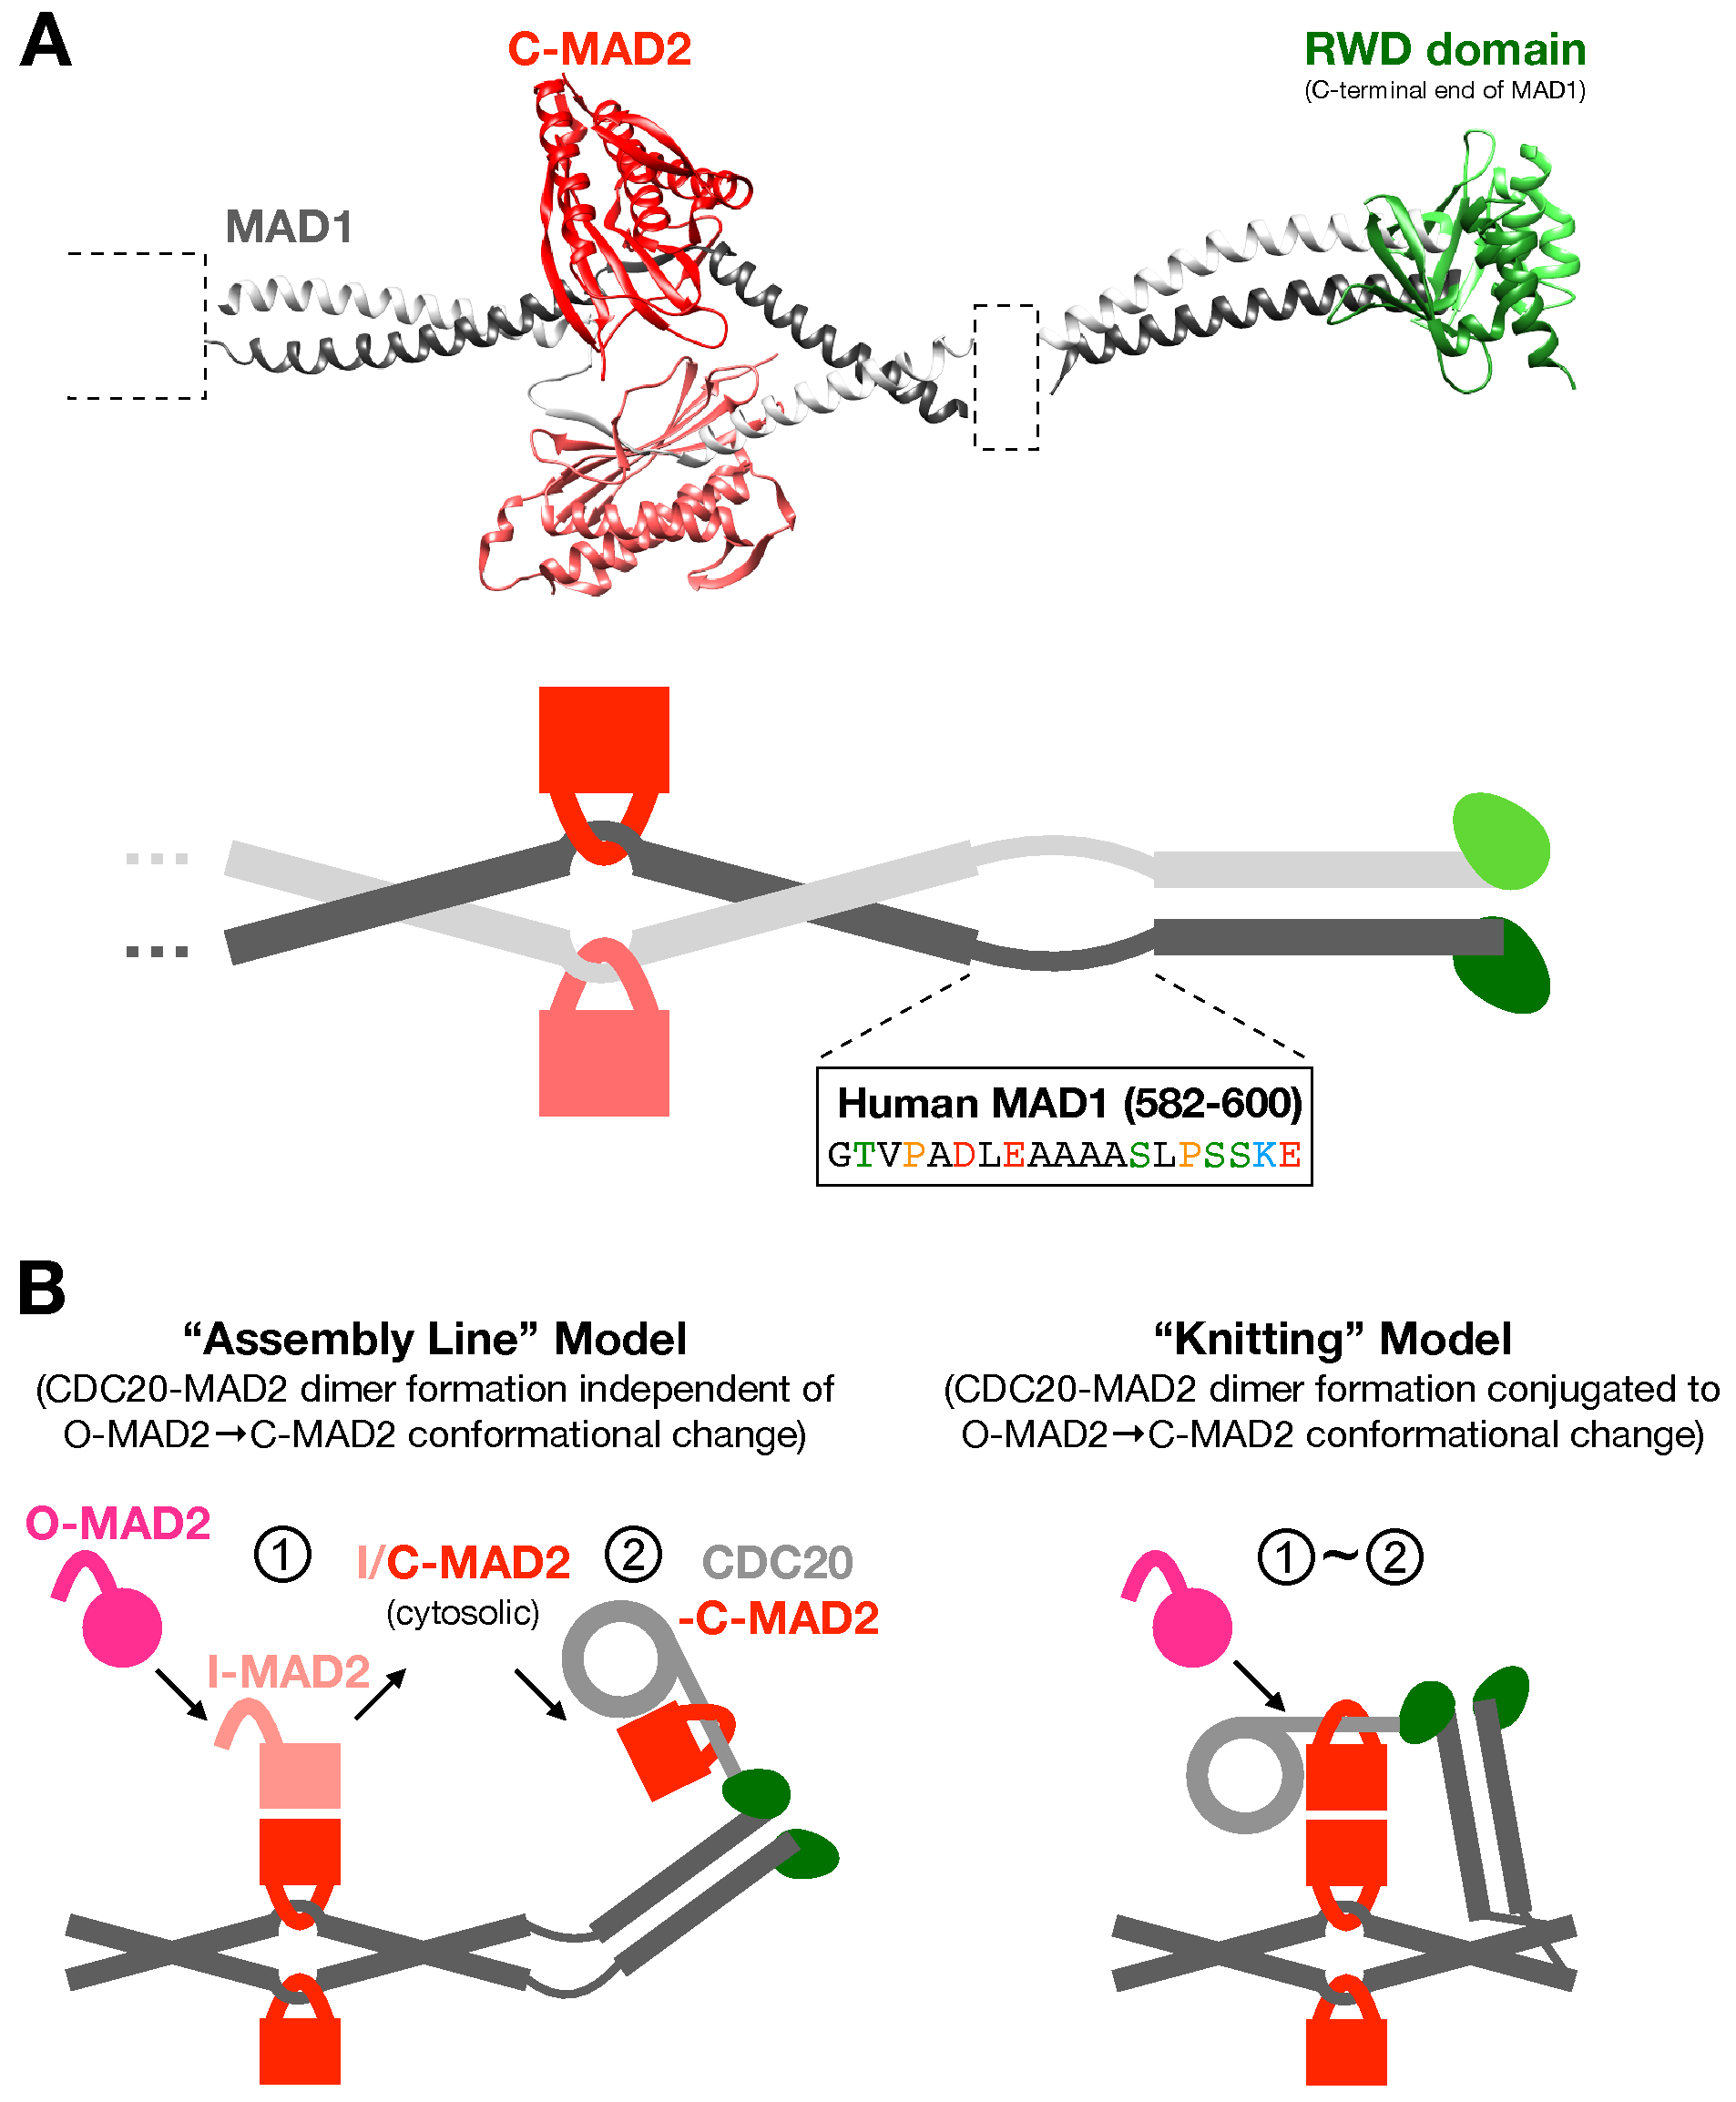
\includegraphics[width=0.75\textwidth]{chapters/figures/MAD1C+KnittingModel.pdf}
    \phantomsubfiglabel{HsMAD1CTerStructure} % subfigure A
    \phantomsubfiglabel{TwoModelCartoons} % subfigure B
    \caption{\textbf{The structure of the \protein{Mad1}-\protein{Mad2} heterotetramer and the two models of the molecular mechanism of the formation of \protein{Cdc20}-\protein{Mad2}.}}
    \noindent\justifying (A) Top panel: the known structure of the \protein{Mad1}-\protein{Mad2} heterotetramer. PDB IDs: 1GO4 (left, \cite{Structure1GO4}), 4DZO (right, \cite{Structure4DZO}). Structures of the N-terminus and the segment spanning a.a. 580--597 are unknown. Various secondary structure prediction algorithms consistently predicted this segment to be a flexible loop (though the predicted starting and ending positions may vary among different algorithms). Bottom panel: a cartoon illustrating the known structure of the \protein{Mad1}-\protein{Mad2} heterotetramer. The color scheme matches the top panel. To distinguish the two \protein{Mad1} proteins [and their C-terminal RWD domains] and the two \protein{Mad2} proteins, slightly different colors are applied. In all cartoons later, both copies will use the same color scheme. The sequence of the loop region (a.a. 582--600) predicted by Lupas' method is shown \cite{LupasCOILS}. Serine/threonine residues are colored green. Proline residues are colored orange. Negatively charged residues are colored red. Lysine residues are colored blue. All cartoons in this chapter are not to scale. (B) The two models of the molecular mechanism of the formation of \protein{Cdc20}-\protein{Mad2}: the "assembly line" model (left) and the "knitting" model (right).
    \label{MAD1C+KnittingModel}
\end{figure}

\begin{figure}
    \centering
    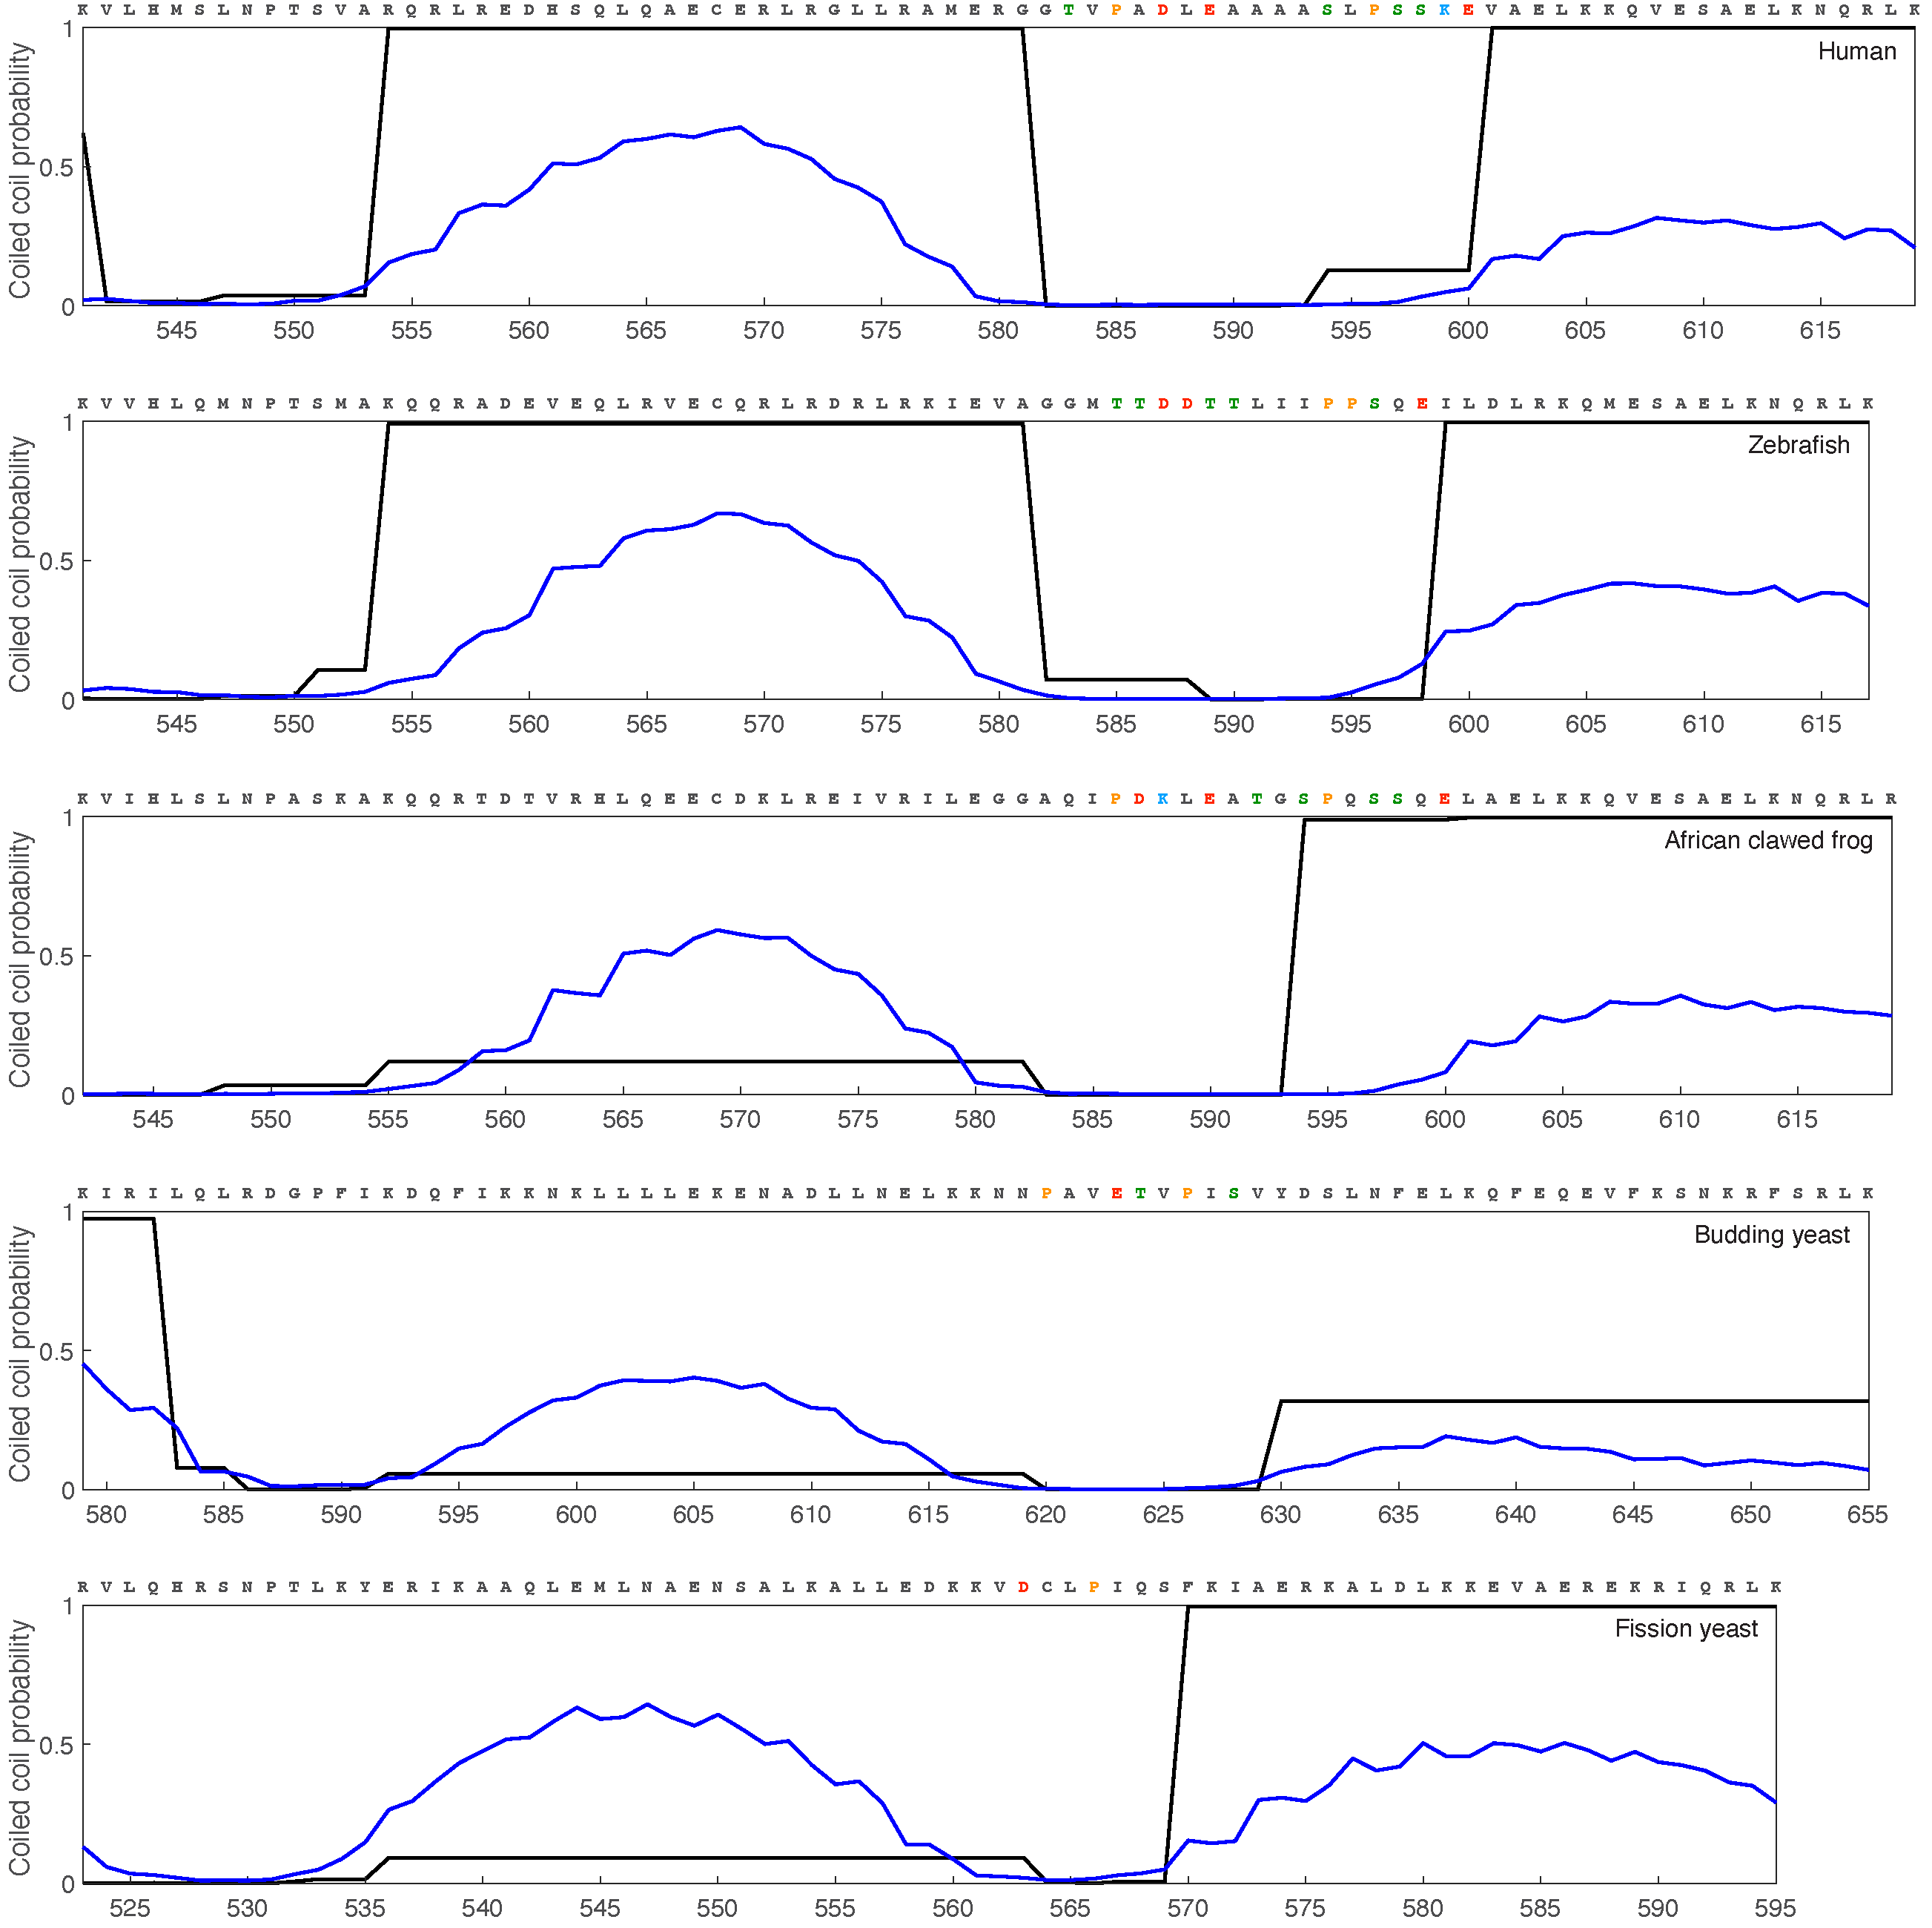
\includegraphics[width=0.89\textwidth]{chapters/figures/MAD1_MIM-RLK_Lupas+DeepCoil2.pdf}
    \caption{\textbf{The secondary structure of \protein{Mad1}'s loop region is well conserved.}}
    \noindent\justifying Although the primary sequence of \protein{Mad1}'s loop region is not conserved, proline residues are commonly (not always) found in this region. The figure shows coiled-coil predictions by two algorithms (black curves: Lupas' method using a gliding window size of 28 residues \cite{LupasCOILS}; blue curves: raw predicted probabilities by DeepCoil2 \cite{DeepCoil}) on the region spanning from \protein{Mad1}'s MIM (which is also not a coiled coil \cite{Structure1GO4}) to \protein{Mad1}'s consensus RLK motif from \Latin{Homo sapiens} (human), \Latin{Danio rerio} (zebrafish), \Latin{Xenopus Laevis} (African clawed frog), \Latin{Saccharomyces cerevisiae} (budding yeast), and \Latin{Schizosaccharomyces pombe} (fission yeast). The $x$-axis represents the coordinates of residues within \protein{Mad1}. The primary sequences of full-length \protein{Mad1} proteins were supplied as the input, but only probability predictions on this region are shown here. The RLK motif directly binds to \protein{Bub1} \cite{Ji2017eLife, BUB1CD1-MAD1CStructure} and is located within the coiled coil leading to the RWD domain (see the crystal structure on the right in \myref{HsMAD1CTerStructure}). Residues within the putative loop region are colored as in \myref{HsMAD1CTerStructure}. Similar prediction results were obtained using MARCOIL \cite{MARCOIL} and PSIPRED 4.0 \cite{PSIPREDOriginal, PSIPREDPlatform} although the exact starting and ending residues of the flexible loop may differ (data not shown).
    \label{MAD1_MIM-RLK_Lupas+DeepCoil2}
\end{figure}

We reason that the ``knitting'' model is more realistic based on many pieces of evidence from previous literature. First, locking cytosolic \protein{Mad2} to its closed conformation inhibited the heterodimerization between \protein{Cdc20} and \protein{Mad2} and compromised the SAC signaling activity \cite{Ma+Poon2016, Ma+Poon2018, Kim2018}, which can be interpreted by the ``knitting'' model. Second, the binding of \protein{Cdc20} to \protein{Mad1}'s RWD domain is suggested to be important to the SAC signaling activity \cite{Kruse2014, SpMad1, Faesen2017, Ji2017eLife}. One explanation is that the binding may increase the local concentration of \protein{Cdc20}, which is better harnessed by the ``knitting'' model. The anchoring of the basic motif of \protein{Cdc20} to \protein{Mad1}'s RWD domain may even topologically hinder the stringing of \protein{Mad2} that is already in the closed conformation because \protein{Cdc20}'s MIM is between the basic motif and the \textbeta{}-propeller. Third, two recent studies strongly supported the spatio-temporal coupling between \protein{Mad2}'s conformational change and the formation of the \protein{Cdc20}-\protein{Mad2} dimer \cite{BUB1-CDC20-MAD1, Tripartite}.

In this chapter, we intend to prove the "knitting" model by introducing mutations to \protein{Mad1} that theoretically only impair the SAC signaling activity if the "knitting" model is correct. It should be noted that there is a gray area between the two models, given that I-\protein{Mad2} can exist in the solution \cite{I-MAD2}, which may be the fresh \protein{Mad2} conformer coming off the template-based conformational switch, entering the cytosolic pool, and eventually binding to \protein{Cdc20} (becoming C-\protein{Mad2} thereafter). We categorize this situation into the "assembly line" model (also illustrated in \myref{TwoModelCartoons}) because our mutational approach should not impair the SAC signaling activity in this case either (see \myref{LoopDeletionSection}).

\section{The \protein{Mad1}-\protein{Mad2} heterotetramer may adopt a fold-back conformation both \Latin{in vivo} and \Latin{in vitro}}
\label{TwoPossibilities}

For the ``knitting'' model to work, the site of \protein{Mad2}'s conformational switch and \protein{Cdc20}'s MIM have to be positioned close enough. According to the crystal structure, the axial length from the MIM to the start of the loop region is about 5--\SI{6}{nm} while the axial length from the end of the loop region to the anchoring point of \protein{Cdc20} is about \SI{7}{nm} \cite{TemplateModel, Ji2017eLife, BUB1-CDC20-MAD1, Structure1GO4, Structure4DZO}. In contrast, if we model the disordered N-terminus of \protein{Cdc20} as a simple 3-D random walk, we can estimate the root-mean-square distance from \protein{Cdc20}'s BOX1 to its MIM (about 90 residues) to be less than \SI{4}{nm}. Due to steric hindrance and restrictions imposed by the Ramachandran plot, such a simple 3-D random walk model is far from realistic. However, even if we apply a more sophisticated worm-like chain model with a persistence length of 3--\SI{4}{\angstrom} \cite{RandomWalk3D-WormLikeChain}, the root-mean-square distance from \protein{Cdc20}'s BOX1 to its MIM is still only about \SI{5}{nm}. These estimations suggest that additional mechanisms may be at work to position the site of \protein{Mad2}'s conformational switch and \protein{Cdc20}'s MIM closely to facilitate the heterodimerization between \protein{Mad2} and \protein{Cdc20}.

One possibility has been suggested in \cite{BUB1-CDC20-MAD1, Tripartite} that the cooperative binding of \protein{Cdc20} to \protein{Mad1}'s RWD domain and \protein{Bub1} helps to unravel the N-terminus of \protein{Cdc20}. Indeed, if the disordered region from \protein{Cdc20}'s BOX1 to its MIM is fully stretched, it will be more than enough for the MIM of the \protein{Cdc20} anchored to \protein{Mad1}'s RWD domain to engage the site of \protein{Mad2}'s conformational switch. However, there are conflicting claims over whether and where \protein{Bub1} directly binds to \protein{Mad1} \cite{Ji2017eLife, BUB1-CDC20-MAD1, BUB1CD1-MAD1CStructure}. If \protein{Bub1}'s conserved domain 1 (CD1, which is also named conserved motif 1 or CM1) directly interacts with \protein{Mad1}'s consensus RLK motif located in \protein{Mad1}'s C-terminal coiled coil \cite{Ji2017eLife, BUB1CD1-MAD1CStructure} (illustrated in \myref{KnittingModel} as the contact between \protein{Bub1} and the C-terminal coiled coil of \protein{Mad1}), the cooperative binding of \protein{Cdc20} to \protein{Bub1} and \protein{Mad1} may not unravel \protein{Cdc20}'s N-terminus because the segment of \protein{Bub1} from CD1 to ABBA-consensus KEN motifs (which bind to \protein{Cdc20} \cite{BUB1-CDC20-MAD1, CDC20-KEN, ABBA}) is also largely disordered (predicted by AlphaFold2 with low confidence; data not shown).

Another possibility has been suggested in \cite{Structure1GO4, SpMad1} that \protein{Mad1} may position the site of \protein{Mad2}'s conformational switch and \protein{Cdc20}'s MIM closely by assuming a fold-back conformation. As mentioned in the previous section, the secondary structure of \protein{Mad1}'s C-terminal loop region is conserved, whose flexibility may enable such fold-back conformation according to the prediction by the ColabFold advanced algorithm (see \myref{MAD1_ColabFoldPrediction}, which is close to the scenario envisioned by \cite{SpMad1}). If we truncate residues 582--600 of human \protein{Mad1}, which removes the flexible loop and fuses the coiled coils upstream and downstream of the loop region (while preserving the original heptad repeat position designation as assigned by Lupas' method \cite{LupasCOILS} as well as DeepCoil2 \cite{DeepCoil}; data not shown), the resulting loop-deleted \protein{Mad1} (henceforth referred to as \protein{Mad1}\textDelta{}L) homodimer can only assume an extended conformation (see \myref{MAD1DeltaL_ColabFoldPrediction}).

\begin{figure}
    \centering
    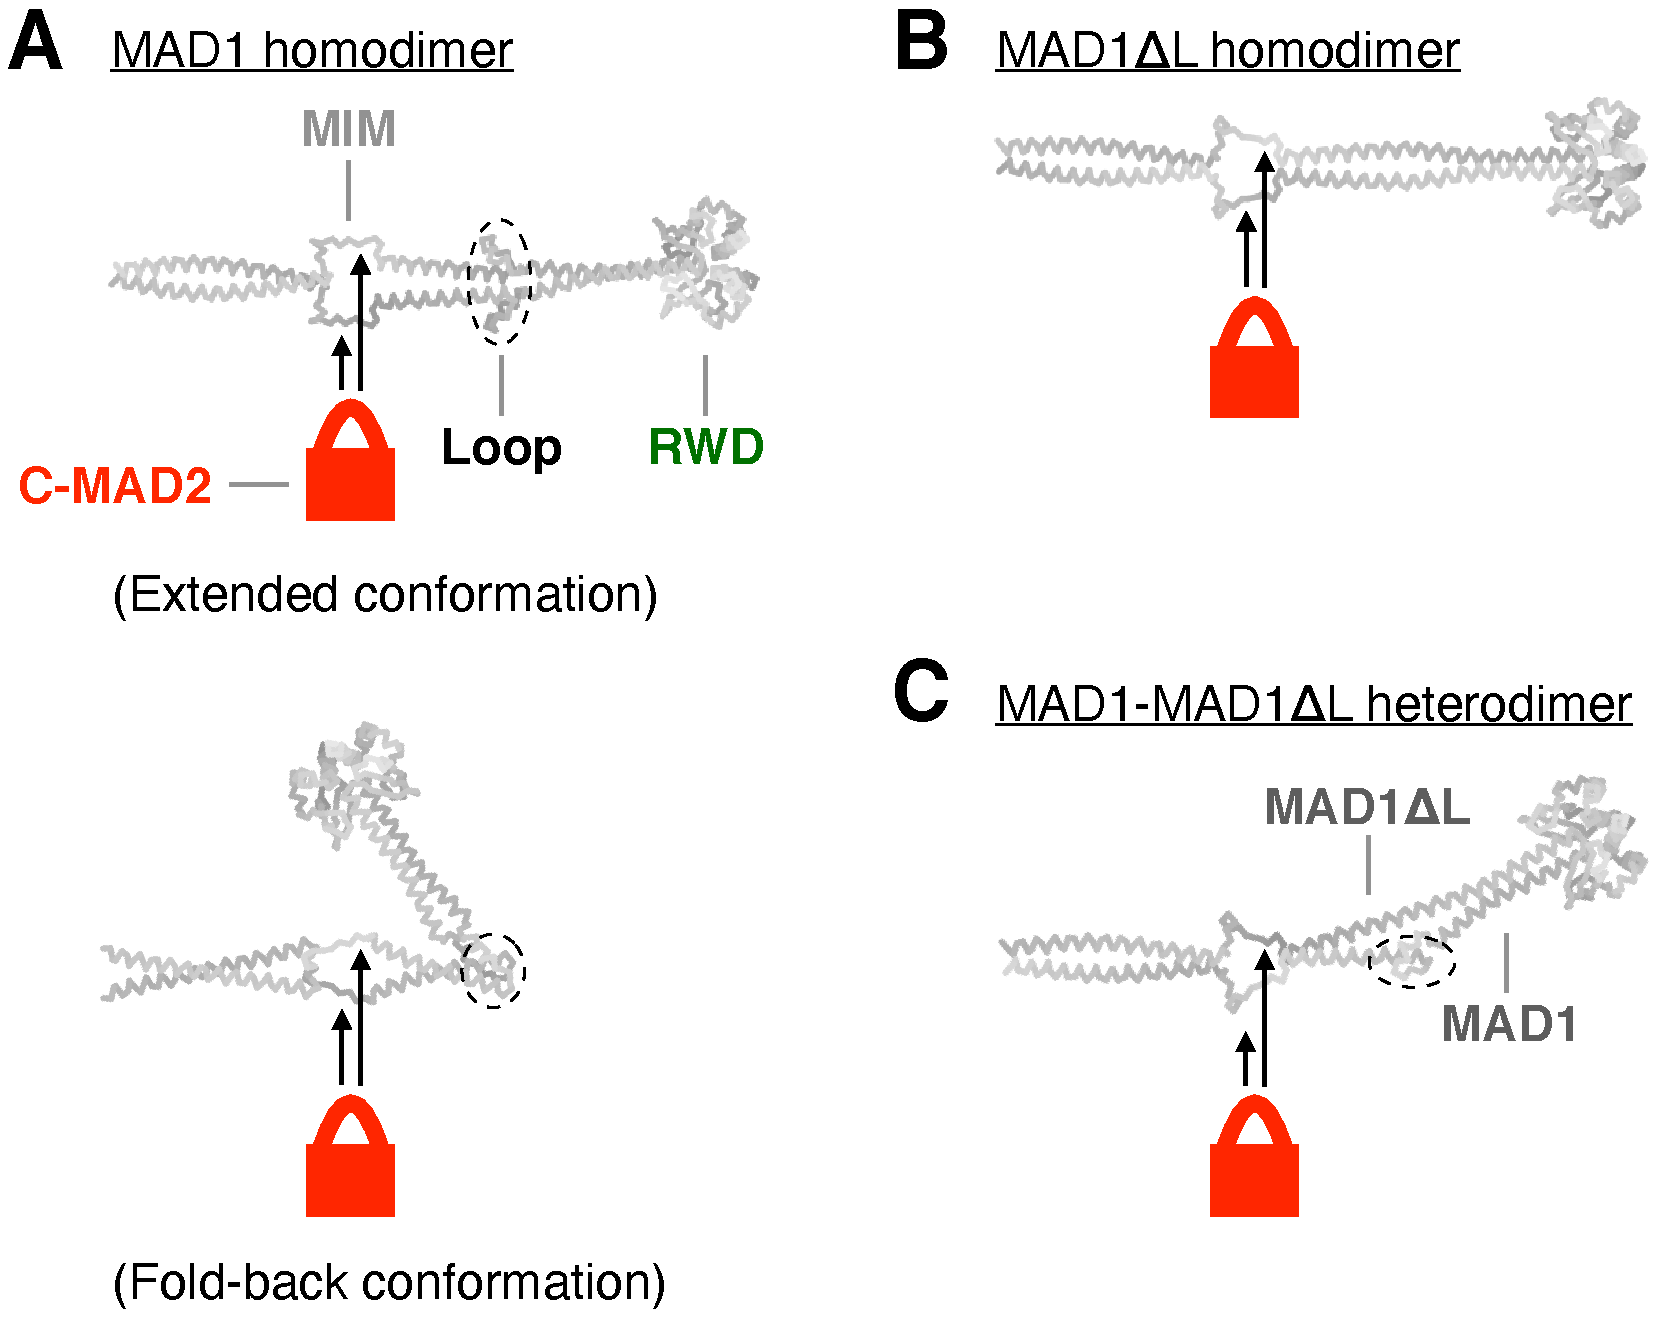
\includegraphics[width=0.85\textwidth]{chapters/figures/ColabFoldPrediction.pdf}
    \phantomsubfiglabel{MAD1_ColabFoldPrediction} % subfigure A
    \phantomsubfiglabel{MAD1DeltaL_ColabFoldPrediction} % subfigure B
    \phantomsubfiglabel{MAD1-MAD1DeltaL_ColabFoldPrediction} % subfigure C
    \caption{\textbf{Representative structures of the C-terminus of the \protein{Mad1} homodimer, the \protein{Mad1}\textDelta{}L homodimer, and the \protein{Mad1}-\protein{Mad1}\textDelta{}L heterodimer were predicted by ColabFold.}}
    \noindent\justifying Representative models (out of five models in total) of the C-terminus of the \protein{Mad1} homodimer (A), the \protein{Mad1}\textDelta{}L homodimer (B), and the \protein{Mad1}-\protein{Mad1}\textDelta{}L heterodimer (C) were predicted by ColabFold using the default parameter settings of ColabFold advanced algorithm. The loop region of wildtype \protein{Mad1} is circled out in (A) and (C). The MIM of \protein{Mad1} where C-\protein{Mad2} binds and the RWD domain at the C-terminal end of \protein{Mad1} where the N-terminal BOX1 of \protein{Cdc20} is anchored are also indicated. The C-terminus of the \protein{Mad1} homodimer may assume a fold-back conformation [see the bottom panel of (A)]. In the predicted structure of the \protein{Mad1}-\protein{Mad1}\textDelta{}L heterodimer, the loop region of the wildtype copy introduces a bulge but the overall conformation is extended. 
    \label{ColabFoldPrediction}
\end{figure}

To confirm such fold-back of \protein{Mad1}, we first noted that about 37\% of purified full-length \protein{Mad1}-\protein{Mad2} heterotetramers do not show distinguishable \protein{Mad1}-MIM-\protein{Mad2} and \protein{Mad1}-RWD domain densities as visualized by electron microscopy using metal shadowing \cite{BUB1-CDC20-MAD1}. This may be explained by that this population of \protein{Mad1}-\protein{Mad2} heterotetramers assumes a fold-back conformation. To further support that the \protein{Mad1} may assume a fold-back conformation \Latin{in vivo}, we resorted to the distance-sensitive FRET measurement. We fused the donor fluorophore mNeonGreen to the C-terminal end of \protein{Mad1} (see \myref{TaggingSACProteins}) and inserted the acceptor fluorophore mScarlet-I into the \textbeta{}5-\textalpha{}C loop of \protein{Mad2} \cite{mSI, beta5-alphaCLoop} (the recombinant protein is henceforth referred to as ``\protein{Mad2}$\wedge$mScarlet-I''; see \myref{MAD2InternalTagging_Strategy}). If the heterotetramer always assumes an extended conformation, the distance between the donor and acceptor will be larger than \SI{10}{nm}, which allows no or minimal FRET between the donor \protein{Mad1}-mNG and the acceptor \protein{Mad2}$\wedge$mScarlet-I \cite{Kukreja2020}. However, if the heterotetramer may assume a fold-back conformation, the distance between the donor and acceptor may be reduced to allow for FRET between the donor and the acceptor.

\begin{figure}
    \centering
    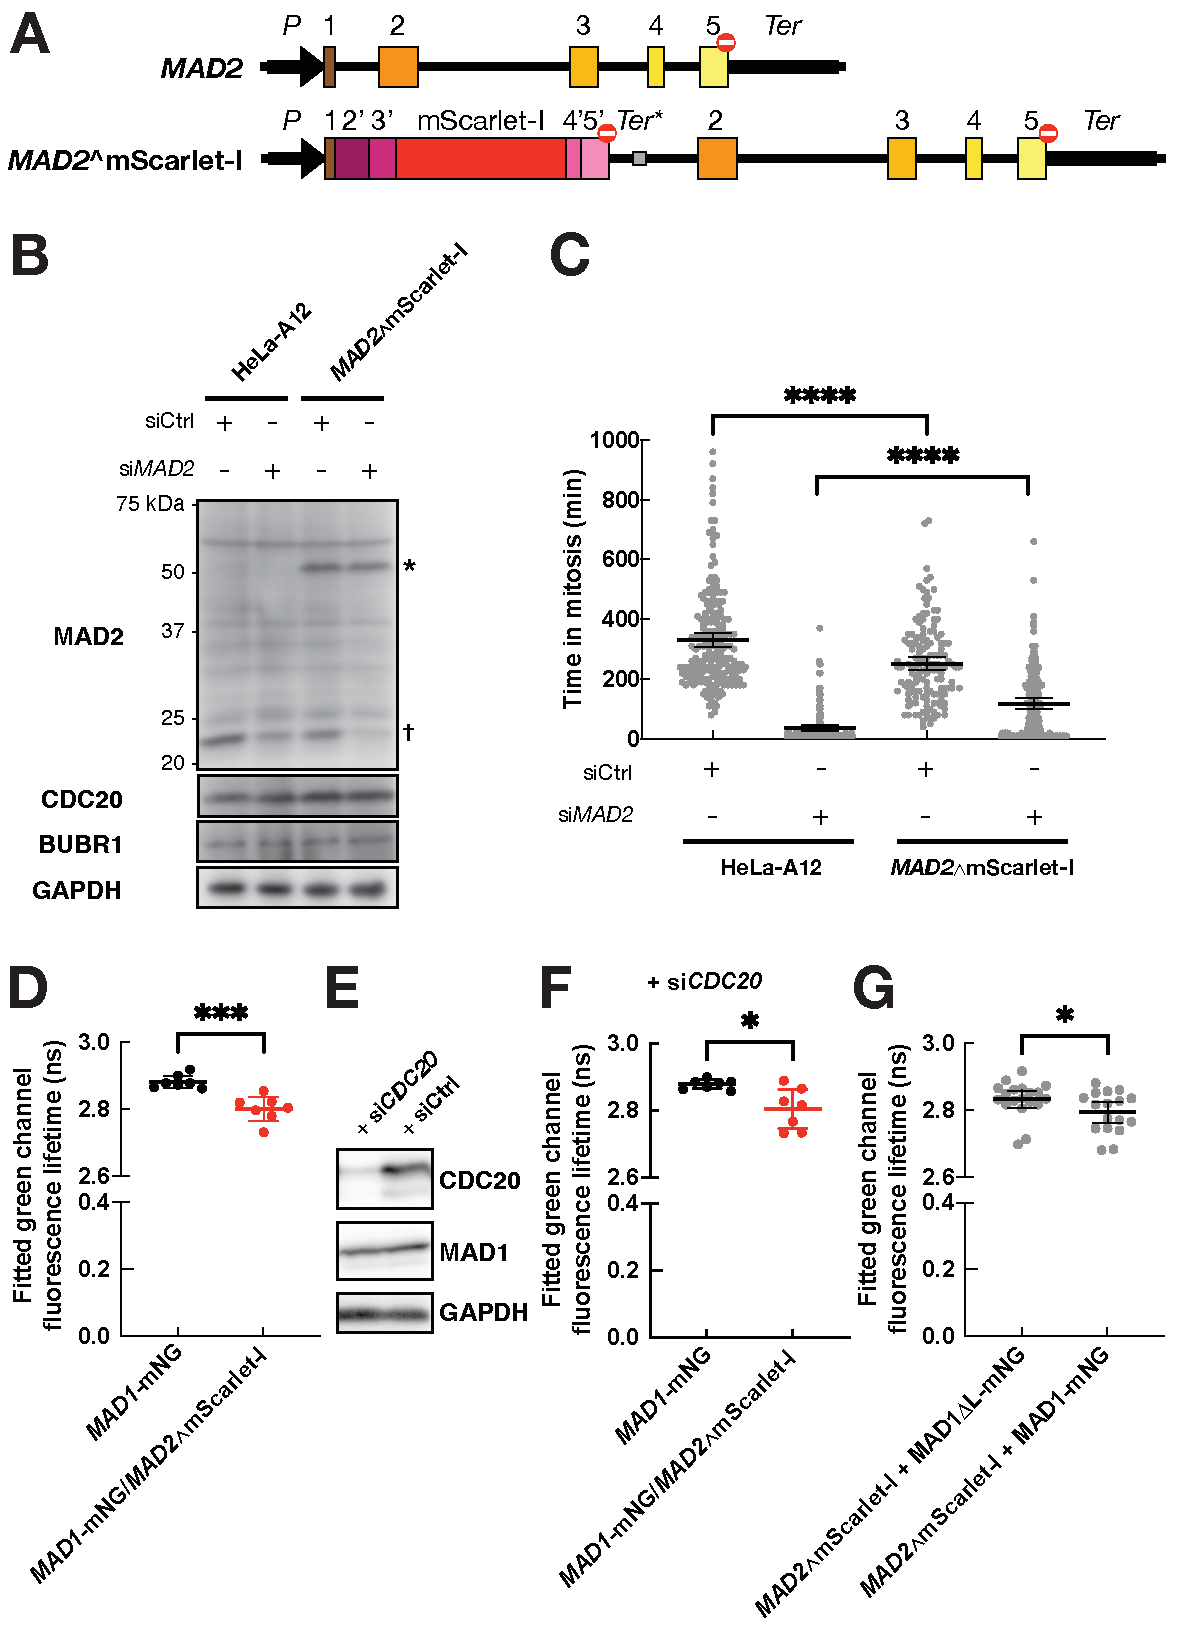
\includegraphics[width=0.91\textwidth]{chapters/figures/InternallyTaggedMAD2+NPCFLIM.pdf}
    \phantomsubfiglabel{MAD2InternalTagging_Strategy} % subfigure A
    \phantomsubfiglabel{MAD2InternalTagging_WB} % subfigure B
    \phantomsubfiglabel{MAD2InternalTagging_SACActivity} % subfigure C
    \phantomsubfiglabel{NosiCDC20_FLIM} % subfigure D
    \phantomsubfiglabel{siCDC20_WB} % subfigure E
    \phantomsubfiglabel{siCDC20_FLIM} % subfigure F
    \caption{\textbf{The observation of FRET between \protein{Mad1}-mNG and \protein{Mad2}$\wedge$mScarlet-I at the interphase/prophase NPC suggested that \protein{Mad1}-\protein{Mad2} heterotetramers may assume a fold-back conformation \Latin{in vivo}.}}
    \label{InternallyTaggedMAD2+NPCFLIM}
\end{figure}
\begin{figure}
    \noindent\justifying \textbf{(Caption of \myref{InternallyTaggedMAD2+NPCFLIM} continued from a previous page)} (A) Diagram of the endogenous gene{Mad2} allele and the genome-edited \gene{Mad2}$\wedge$mScarlet-I allele. Boxes 1--5 represent the exons. The regions between these boxes represent the introns. Boxes 2'--5' encode the same peptides as boxes 2--5 respectively, with the introduction of certain silence mutations that make the recombinant \protein{Mad2}$\wedge$mScarlet-I resistant to si\gene{Mad2}. The black ``\textit{P}'' arrow represents the promoter and the 5'-UTR. The black ``\textit{Ter}'' bar represents the 3'-UTR and the polyadenylation signal. The gray ``\textit{Ter}*'' bar represents the polyadenylation signal of rabbit \textbeta{}-globin. The red stop signs represent stop codons. The sequence of the \gene{Mad2}$\wedge$mScarlet-I allele was confirmed by genotyping and Sanger sequencing (data not shown). (B) Immunoblotting showed that \protein{Mad2}$\wedge$mScarlet-I (labeled by an asterisk, with an expected molecular weight of \SI{51.0}{kDa}) was correctly expressed in the heterozygous \gene{Mad2}$\wedge$mScarlet-I HeLa-A12 cell line and was resistant against si\gene{Mad2}. As a comparison, wildtype \protein{Mad2} (labeled by a cruciform with a molecular weight of \SI{23.5}{kDa}) was effectively knocked down by si\gene{Mad2}. The immunoblot against GAPDH served as the loading control. (C) Unsynchronized cells were treated with respective siRNAs for one day, treated with \SI{50}{nM} nocodazole. Each gray dot represents a cell. The total number of cells in each group $N > 140$. Mean values $\pm 95\%$ confidence intervals are overlaid. Unpaired $t$-tests with Welch's correction were performed in Prism 9. Results are representative of two independent experiments. (D) The average lifetime of \protein{Mad1}-mNG in the \gene{Mad1}-mNG or the \gene{Mad1}-mNG/\gene{Mad2}$\wedge$mScarlet-I double genome-edited HeLa-A12 cell  line using a two-component exponential decay to fit the raw data of FLIM. Each dot represents a single cell. Mean values $\pm 95\%$ confidence intervals are overlaid. The total number of cells in each group $N = 7$. Results are representative of two independent experiments. Unpaired $t$-tests with Welch's correction were performed in Prism 9. (E) Unsynchronized HeLa-A12 cells were treated with si\gene{Cdc20} or a control siRNA for \SI{2}{d} and probed for \protein{Cdc20}, \protein{Mad1}, and GAPDH (loading control). (F) Same as (D), except that cells were treated with si\gene{Cdc20} as in (E).
\end{figure}

We confirmed the expression of full-length \protein{Mad2}$\wedge$mScarlet-I in the heterozygous \gene{Mad2}$\wedge$mScarlet-I genome-edited HeLa-A12 cell line (see \myref{MAD2InternalTagging_WB}), wherein the expression level of either \protein{BubR1} or \protein{Cdc20} was not affected. \protein{Mad2}$\wedge$mScarlet-I could support a certain degree of the SAC signaling activity when the endogenous wildtype \protein{Mad2} was knocked down (see \myref{MAD2InternalTagging_SACActivity}). Using fluorescence lifetime imaging microscopy (FLIM) \cite{FLIM}, we quantified a FRET efficiency of about 3\% between \protein{Mad1}-mNG and \protein{Mad2}$\wedge$mScarlet-I at the interphase/prophase NPC in the heterozygous \gene{Mad1}-mNG, \gene{Mad2}$\wedge$mScarlet-I genome-edited HeLa-A12 cell line (see \myref{NosiCDC20_FLIM,FLIMMethod}). We chose to measure FRET at the interphase/prophase NPC to facilitate data collection by the line-scanning confocal microscope and to avoid the potential intermolecular FRET between a donor from one \protein{Mad1}-\protein{Mad2} heterotetramer and an acceptor from another nearby heterotetramer at the corona of a signaling kinetochore. This FRET persisted even when \gene{Cdc20} was knocked down by RNAi (see \myref{siCDC20_WB,siCDC20_FLIM}), which indicates that this FRET does not depend on \protein{Mad1}'s catalytic role but is rather intrinsic to the structural characteristics of the \protein{Mad1}-\protein{Mad2} heterotetramer. Although we still cannot completely rule out potential intermolecular FRET, we confirmed the existence of the anticipated FRET that may result from the fold-back of \protein{Mad1} \Latin{in vivo}.

\section{\protein{Mad1}'s loop region is important to the SAC signaling activity \Latin{in vivo}}
\label{LoopDeletionSection}

We next sought to determine whether the loop region of \protein{Mad1} that likely enables the fold-back conformation is important to the SAC signaling activity \Latin{in vivo}. We integrated the expression cassette of either \protein{Mad1}-mNG or \protein{Mad1}\textDelta{}L-mNG into the genome of HeLa-A12 cells using Cre-\bacterialgene{lox} RMCE (see \myref{Cre-lox}). We then knocked down endogenous \protein{Mad1} in these cells using two siRNAs that target the 3'-UTR of \gene{Mad1} \cite{siMAD1-3UTR} (henceforth collectively referred to as si\gene{Mad1}'s) and induced the expression of \protein{Mad1}(WT/\textDelta{}L)-mNG (si\gene{Mad1}-resistant due to the lack of the endogenous 3'-UTR) by doxycycline. Our genome-edited \gene{Mad1}-mNG HeLa-A12 cell line served as the reference for the endogenous level of \protein{Mad1} in live-cell fluorescence imaging.

We found out that knocking down \gene{Mad1} crippled the SAC signaling activity (see \myref{MAD1Rescue_Main}), although cells with less than 10\% of the physiological level of \protein{Mad1} on average (see \myref{MAD1Rescue_WB}) still arrested in mitosis for hours when treated with \SI{100}{nM} nocodazole (only about two hours less than the control group with a physiological level of \protein{Mad1}). Increasing the dosage of si\gene{Mad1}'s did not further decrease the SAC activity, reinforcing that even a small pool of \protein{Mad1} could sustain a considerable level of SAC signaling activity (see \myref{MAD1Rescue_LimitPushing}).

\begin{figure}
    \centering
    \includegraphics[trim={0 0 0 19cm},clip,width=\textwidth]{chapters/figures/MAD1Rescue.pdf}
    \phantomsubfiglabel{MAD1Rescue_Main} % subfigure A
    \phantomsubfiglabel{MAD1Rescue_LimitPushing} % subfigure B
    \phantomsubfiglabel{MAD1Rescue_HeterodimerizationWB} % subfigure C
    \phantomsubfiglabel{MAD1Rescue_Localization} % subfigure D
    \phantomsubfiglabel{MAD1Rescue_WB} % subfigure E
    \caption{\textbf{The loop region of \protein{Mad1} is critical to the SAC signaling activity in its own right.}}
    \label{MAD1Rescue}
\end{figure}
\begin{figure}
    \noindent\justifying \textbf{(Caption of \myref{MAD1Rescue} continued from a previous page)} (A) The first two columns on the left used the \gene{Mad1}-mNG genome-edited HeLa-A12 cell line which served as a reference of the endogenous level of \gene{Mad1}. \Latin{In situ} tagging of \gene{Mad1} did not affect the 3'-UTR which si\gene{Mad1}'s target. The effectiveness of si\gene{Mad1}'s against the \gene{Mad1}-mNG allele was confirmed by the greatly diminished green channel fluorescence signal (data not shown). The two columns on the right used Cre-\bacterialgene{lox} RMCE HeLa-A12 cell lines which were treated with si\gene{Mad1}'s and induced to express either \protein{Mad1}-mNG or \protein{Mad1}\textDelta{}L-mNG. Each dot represents a cell ($N \geq 50$ in each group). Results were pooled from at least two technical repeats. The mean value $\pm$ the 95\% confidence interval of each group is overlaid. Unpaired $t$-tests with Welch's correction were performed in Prism 9. (B) The conditions of si\gene{Mad1} treatment were (from left to right): untreated, \SI{40}{nM} each for two days (the standard condition used throughout this study), \SI{100}{nM} each for two days, \SI{100}{nM} each in day one and \SI{100}{nM} each again in day two. The \gene{Mad1}-mNG genome-edited HeLa-A12 cell line was used in each group. Each dot represents a cell ($N \geq 145$ in each group). The mean value $\pm$ the 95\% confidence interval of each group is overlaid. Welch's ANOVA test [$W(\text{DF}n, \text{DF}d) = 0.9885 (2.000, 298.9)$, $p = 0.3733$] was performed for the three columns on the right. The ANOVA test and the unpaired $t$-test with Welch's correction were done in Prism 9. (C) Using immunoblotting to evaluate the immunoprecipitation by the mNeonGreen-Trap Agarose. The cruciform symbol represents the endogenous \protein{Mad1} band. The expected molecular weights of the recombinant \protein{Mad1}-mNG, \protein{Mad1}\textDelta{}L-mNG, and mNeonGreen are \SI{110.2}{kDa}, \SI{108.4}{kDa}, and \SI{26.9}{kDa}, respectively. The immunoblot against GAPDH served as the loading control. Blots shown here are from the same immunoprecipitation experiment representative of two independent repeats. (D) The \gene{Mad2}$\wedge$mScarlet-I genome-edited HeLa-A12 treated with si\gene{Mad1}'s and rescued by \protein{Mad1}(WT/\textDelta{}L)-mNG were imaged using wide-field fluorescence microscopy. Cells were arrested at mitosis using a thymidine--nocodazole synchronization protocol (see \myref{WBMethods}). Representative micrographs are shown in the top panel. Maximum $z$-projected green channel images shown here share the same LUT. Maximum $z$-projected red channel images shown here also share the same LUT. Scale bar, \SI{10}{\micro m}. Due to various expression levels of induced \protein{Mad1}(WT/\textDelta{}L)-mNG in different cells, signaling kinetochores were filtered by the localization of \protein{Mad1}(WT/\textDelta{}L)-mNG (with an arbitrary threshold of 1000--\SI{7000}{AU}). Each gray dot represents a single signaling kinetochore ($N \geq 85$ in each group). The mean value $\pm$ the 95\% confidence interval of each group is overlaid. Unpaired $t$-tests with Welch's correction were performed in Prism 9. (E) Knockdown of the endogenous \gene{Mad1} by si\gene{Mad1}'s had an efficiency of over 90\% based on the intensity of the residual \protein{Mad1} band. The cellular abundance of either \protein{BubR1}, \protein{Cdc20}, or \protein{Bub3} was not affected. The immunoblot against GAPDH served as the loading control. Unsynchronized Cre-\bacterialgene{lox} RMCE HeLa-A12 cells were used.
\end{figure}

Surprisingly, \protein{Mad1}\textDelta{}L-mNG had impaired support for the SAC in a dominant-negative manner: cells treated with si\gene{Mad1}'s and rescued by a physiological level of \protein{Mad1}\textDelta{}L-mNG arrested in mitosis for a significantly shorter duration than cells which were not rescued. As a comparison, wildtype \protein{Mad1}-mNG fully restored the SAC signaling activity (see \myref{MAD1Rescue_Main}). One possible explanation was that \protein{Mad1}\textDelta{}L-mNG might dimerize with the remaining endogenous \protein{Mad1} and restrict its structural flexibility. Structural prediction of the heterodimer between wildtype \protein{Mad1} and \protein{Mad1}\textDelta{}L showed that the loop region of the wildtype copy introduced a bulge but could not enable a fold-back conformation of the heterodimer due to stiffness of the fused \textalpha{}-helices of the \protein{Mad1}\textDelta{}L counterpart (see \myref{MAD1-MAD1DeltaL_ColabFoldPrediction}). To prove this hypothesis, we pulled down doxycycline-induced \protein{Mad1}(wildtype/\textDelta{}L)-mNG from lysates of HeLa-A12 cells in which endogenous \protein{Mad1} was not knocked down. We found that endogenous \protein{Mad1} was also pulled down by both \protein{Mad1}-mNG and \protein{Mad1}\textDelta{}L-mNG, but not by mNeonGreen alone (see \myref{MAD1Rescue_HeterodimerizationWB}). We further confirmed that \protein{Mad1}\textDelta{}L-mNG did not cause defects in the localization of the \protein{Mad1}\textDelta{}L-\protein{Mad2} heterotetramer (see \myref{MAD1Rescue_Localization}) or the expression of \protein{BubR1}, \protein{Cdc20}, or \protein{Bub3} (see \myref{MAD1Rescue_WB}). \Latin{In vitro} reconstitution data from our collaborators (not shown here) also suggested that truncating the loop region of \protein{Mad1} reduced the formation rate of \protein{Cdc20}-\protein{Mad2}. Therefore, although the results of our knockdown-rescue experiments were hindered by the incomplete knockdown of the endogenous \protein{Mad1}, all evidence combined suggested that the loop region of \protein{Mad1} is critical to the SAC signaling activity in its own right.

\section{\protein{Mad1}(Lmut) can fully support the SAC signaling activity}
% The function of \protein{Mad1}'s loop region does not depend on the potential phosphorylation of any serine or threonine residues within it

Many possibilities could underlie the observation that the deleted segment encompassing residues 582--600 in \protein{Mad1}\textDelta{}L is important to the SAC signaling activity. It is known that S598 can be phosphorylated by \protein{Mps1} \Latin{in vitro} \cite{MAD1_pS598}. There could also be a certain unknown protein-protein interaction associated with the loop region of \protein{Mad1} that is important to the SAC. To prove that it is the structural flexibility provided by the loop region that is critical to the SAC signaling activity, we tested two different artificial flexible loops to replace the original segment encompassing residues 582--600: ``AL11'' and ``Lmut'' (see \myref{AL11+Lmut_Lupas+DeepCoil2}). Both of them consist of 19 amino acid residues like the original one. AL11 is a previously characterized flexible linker composed of 11 alanine residues, 7 glycine residues, and 1 threonine residue \cite{AL11}. In Lmut, serine and threonine residues of the original segment are mutated into alanine and valine residues, respectively. The amino acids between the two prolines are adjusted into mostly alanine-glycine-alanine repeats while the proline residues themselves and their N-terminal neighboring residues are preserved. % AL11 starts with glycine-threonine at the N-terminus like the endogenous segment.

\begin{figure}
    \centering
    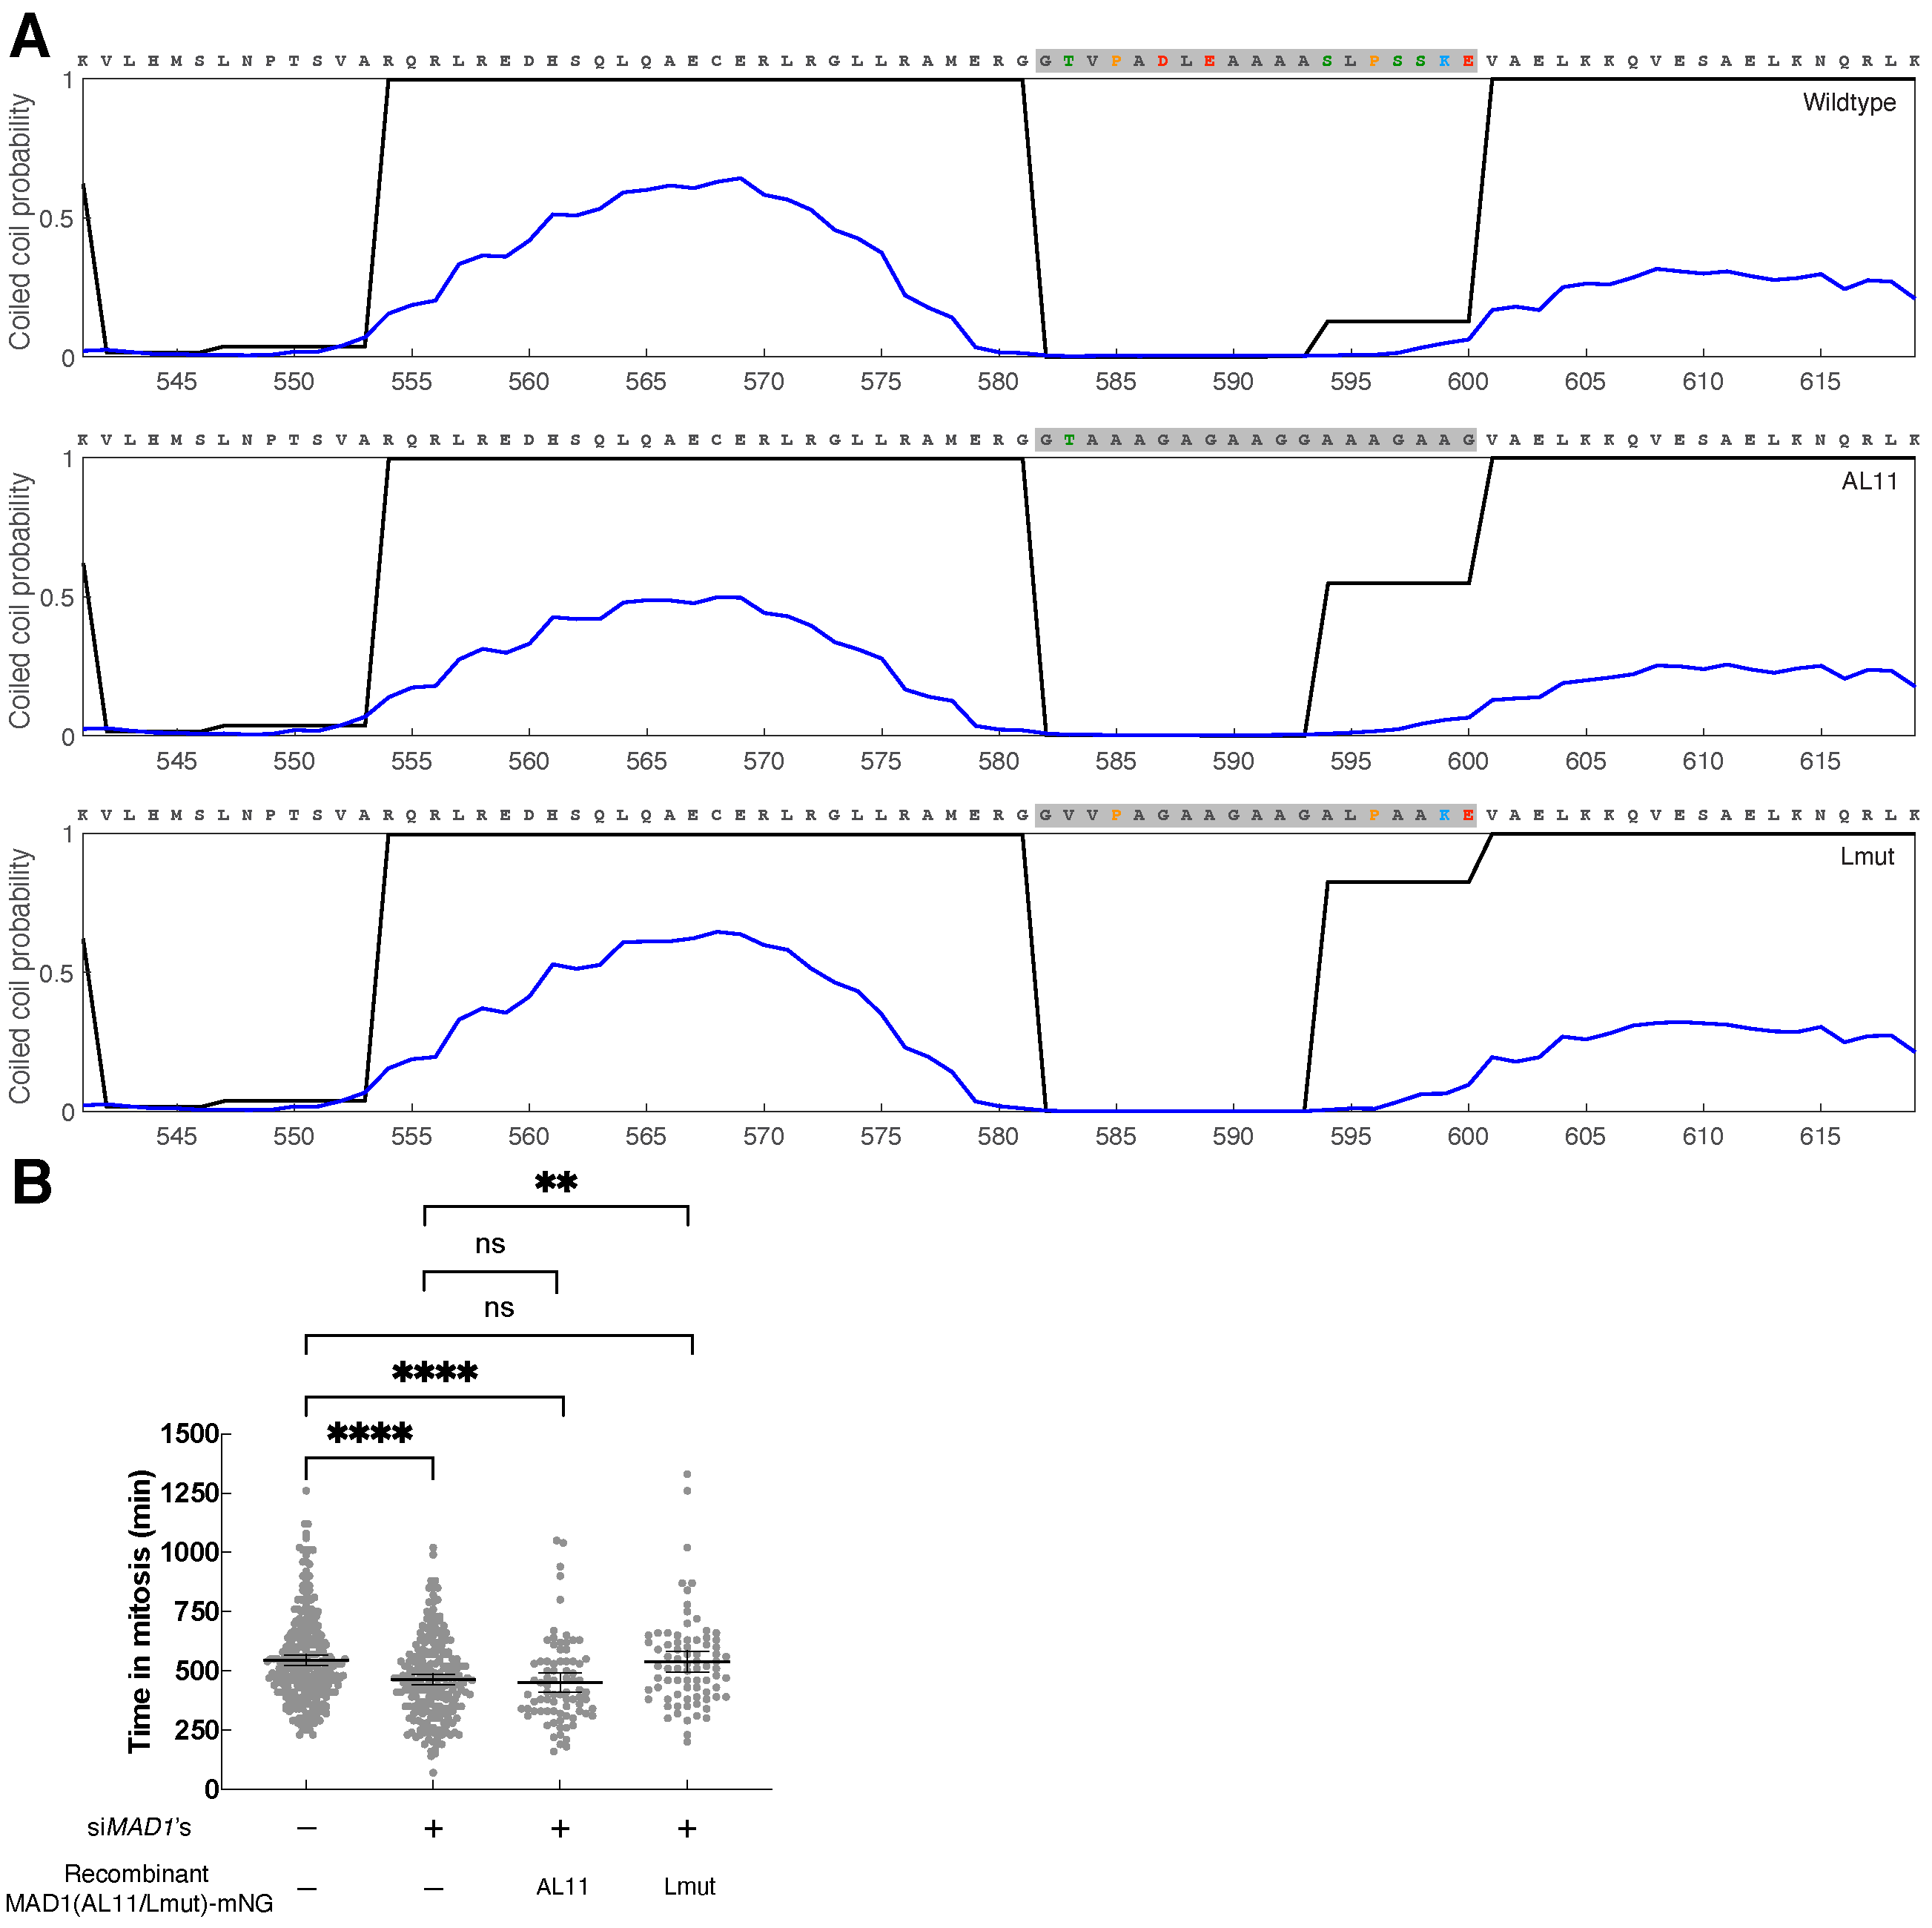
\includegraphics[width=0.95\textwidth]{chapters/figures/AL11+Lmut.pdf}
    \phantomsubfiglabel{AL11+Lmut_Lupas+DeepCoil2} % subfigure A
    \phantomsubfiglabel{AL11+Lmut_Rescue} % subfigure B
    \caption{\textbf{\protein{Mad1}(AL11)-mNG cannot fully rescue the SAC signaling activity but \protein{Mad1}(Lmut)-mNG can.}}
    \noindent\justifying (A) The figure shows coiled-coil predictions of human wildtype \protein{Mad1} (top), \protein{Mad1}(AL11) (middle), \protein{Mad1}(Lmut) (bottom) by the two algorithms as in \myref{MAD1_MIM-RLK_Lupas+DeepCoil2}. The top panel is reproduced from \myref{MAD1_MIM-RLK_Lupas+DeepCoil2}. Segments encompassing residues 582--600 are highlighted by gray boxes. (B) The first two columns on the left used the \gene{Mad1}-mNG genome-edited HeLa-A12 cell line which served as a reference of the endogenous level of \gene{Mad1}. The AllStars negative control siRNA was added to the first group and si\gene{Mad1}'s were added to the second group. The two columns on the right used the Cre-\bacterialgene{lox} RMCE HeLa-A12 cell lines which were treated with si\gene{Mad1}'s and induced to express either \protein{Mad1}(AL11)-mNG or \protein{Mad1}(Lmut)-mNG. Each dot represents a cell ($N \geq 75$ in each group). Results were pooled from at least two technical repeats. The mean value $\pm$ the 95\% confidence interval of each group is overlaid. Unpaired $t$-tests with Welch's correction were performed in Prism 9.
    \label{AL11+Lmut}
\end{figure}

Both \protein{Mad1}(AL11) and \protein{Mad1}(Lmut) were predicted to have a similar coiled-coil propensity profile to that of the endogenous \protein{Mad1} (see \myref{AL11+Lmut_Lupas+DeepCoil2}). Surprisingly, cells treated with si\gene{Mad1}'s and rescued by protein{Mad1}(AL11)-mNG had a lower SAC signaling activity than wildtype cells did (see \myref{AL11+Lmut_Rescue}). As a comparison, \protein{Mad1}(Lmut)-mNG fully restored the SAC signaling activity. We hypothesized that because proline residues may assume the \Latin{cis}-conformation at a higher propensity than many other amino acid residues at equilibrium \cite{Ramachandran1976}, they might facilitate the proper fold-back of \protein{Mad1}.

The fact that Lmut can functionally replace the original segment encompassing residues 582--600 revealed that the SAC likely relies on the structural flexibility but not phosphorylation or unknown protein-protein interactions (other than those that rely solely on the prolines and their N-terminal neighboring residues; see \myref{Chapter4Discussions} for more details) associated with the loop region.

\section{The structural flexibility of \protein{Mad1} enabled by its loop region facilitates the ``knitting'' of the MCC}
\label{FinalKnittingModel}

Based on previous literature and our data, we proposed the following mechanistic model of the catalytic role of \protein{Mad1} in the assembly of \protein{Cdc20}-\protein{Mad2} (see \myref{KnittingModel}). \protein{Mad1} in its fold-back conformation physically positions the MIM of \protein{Cdc20} and \protein{Mad2} closely, facilitating the spatio-temporal coupling of \protein{Mad2}'s conformational switch and the assembly of the \protein{Cdc20}-\protein{Mad2} heterodimer. The avidity binding between the scaffold protein \protein{Mad1} (in its fold-back conformation) and \protein{Cdc20}-\protein{Mad2} energetically favors the formation of the \protein{Mad1}RWD-\protein{Cdc20}-\protein{Mad2}-\protein{Mad1}MIM complex. \protein{Mad1} may switch back to an extended conformation (probably in an ATP-dependent manner), breaking such avidity binding and promoting the release of \protein{Cdc20}-\protein{Mad2} into the cytosol.

\begin{figure}
    \centering
    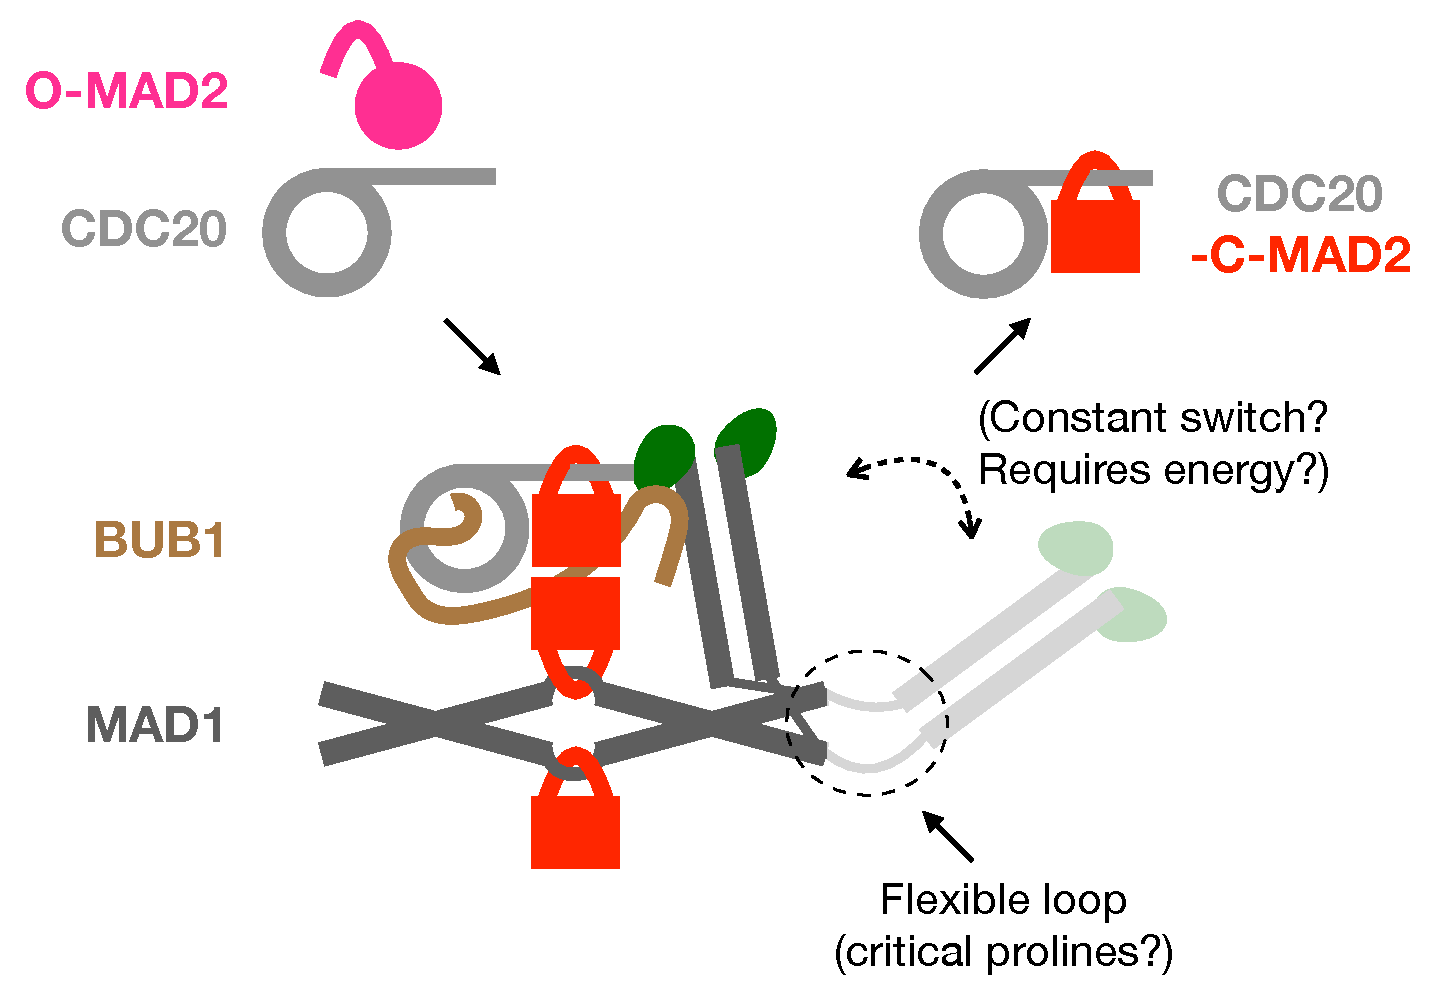
\includegraphics[width=0.75\textwidth]{chapters/figures/KnittingModel.pdf}
    \caption{\textbf{``Knitting'' model: \protein{Mad1}'s structural flexibility may facilitate the spatio-temporal coupling of \protein{Mad2}'s conformational switch and the assembly of the \protein{Cdc20}-\protein{Mad2} heterodimer.}}
    \noindent\justifying The two solid black arrows indicate the formation and release of the \protein{Cdc20}-\protein{Mad2} heterodimer, respectively. T461-phosphorylated CD1 of \protein{Bub1} (458--476) interacts with \protein{Mad1}'s consensus RLK motif located within the coiled coil leading up to the RWD domain \cite{Ji2017eLife, BUB1CD1-MAD1CStructure}. Additionally, the C-terminus of \protein{Bub1}'s CD1 contacts the RWD domain of the opposite \protein{Mad1} copy to whose consensus RLK motif the CD1 interacts with \cite{BUB1CD1-MAD1CStructure}. \protein{Bub1} interacts with \protein{Cdc20} through multiple motifs cooperatively. For example, \protein{Bub1}'s ABBA motif (527--532) binds between Blades 2 and 3 of \protein{Cdc20}'s seven-bladed WD40 fold and \protein{Bub1}'s consensus KEN box (C-terminal to the ABBA motif) likely binds to the center of the top surface of \protein{Cdc20}'s WD40 \cite{BUB1-CDC20-MAD1, CDC20-KEN, ABBA}. \protein{Cdc20} also binds to \protein{Mad1} and \protein{Bub1} cooperatively \cite{BUB1-CDC20-MAD1, Tripartite}. However, whether \protein{Bub1} and \protein{Mad1} cooperate to unravel \protein{Cdc20} and scaffold the assembly of \protein{Cdc20}-\protein{Mad2} is unclear (refer to the two possibilities in \myref{TwoPossibilities}). The proposed avidity binding between the scaffold protein \protein{Mad1} (in its fold-back conformation) and \protein{Cdc20}-\protein{Mad2} involves the \protein{Mad1}RWD-\protein{Cdc20} interaction, the ``safety belt''-like binding between \protein{Cdc20} and \protein{Mad2}, as well as the homodimerization of the \protein{Mad2} in the \protein{Cdc20}-\protein{Mad2} heterodimer and the \protein{Mad2} in the \protein{Mad1}-\protein{Mad2} heterotetramer \cite{TemplateModel, Structure1GO4, beta5-alphaCLoop, I-MAD2, Ji2017eLife, BUB1-CDC20-MAD1}.
    \label{KnittingModel}
\end{figure}

However, there are many missing links towards the ``knitting'' model. For example, do \protein{Bub1} and \protein{Mad1} cooperate to unravel \protein{Cdc20} and scaffold the assembly of \protein{Cdc20}-\protein{Mad2}? Does \protein{Mad1} switch between an extended conformation and the fold-back conformation at a physiologically meaningful rate \Latin{in vivo} and does this switching cycle correlate with the knitting of a \protein{Cdc20}-\protein{Mad2} heterodimer? Does \protein{Mad1}'s conformational switch require energy input? Do the proline residues simply serve to break the coiled coil and shape the flexible loop of \protein{Mad1}, or do they play a more complex role in the proper fold-back of \protein{Mad1}? Future studies are needed to fill these gaps between current experimental evidence and the ``knitting'' model.

\section{Discussions}
\label{Chapter4Discussions}

In this study, we showed for the first time that the \protein{Mad1}-\protein{Mad2} heterotetramer can assume a fold-back conformation both \Latin{in vitro} and \Latin{in vivo}. Our preliminary data indicate that the structural flexibility is enabled by a flexible loop in the C-terminus of \protein{Mad1}, whose secondary structure is conserved. This loop region is important to the SAC signaling activity both \Latin{in vitro} and \Latin{in vivo} and its role does not depend on any potential phospho-regulation of the serine/threonine residues within. We proposed a ``knitting'' model to explain how the structural flexibility of \protein{Mad1}-\protein{Mad2} heterotetramer may facilitate the spatio-temporal coupling between \protein{Mad2}'s conformational change and the formation of \protein{Cdc20}-\protein{Mad2}. It should be noted that even in the absence of \protein{Cdc20}, O-\protein{Mad2} can bind to the \protein{Mad1}-\protein{Mad2} heterotetramer, complete the conformational switch, and dissociate as C-\protein{Mad2} \Latin{in vitro} \cite{Yang2008}. Finding out whether \protein{Cdc20} increases the rate of \protein{Mad2}'s conformational switch will help us further understand the mechanism of the catalysis.

\protein{Mad1} has a long half-life under normal conditions \cite{MAD1MAD2Half-life}. And like \protein{Bub1} \cite{Raaijmakers2018, RZZ-MAD1vsBUB1-MAD1_2018, siROD_Zhang2019}, even a small pool of \protein{Mad1} (at less than 10\% on average of its physiological concentration in our knockdown experiments) can maintain a considerable level of SAC signaling activity in nocodazole-treated cells. Future studies should consider combining RNAi (or induced knockout of \gene{Mad1}) with induced acute degradation of \protein{Mad1} proteins to reduce the contribution of the remaining endogenous \protein{Mad1} homodimer to the SAC signaling activity and to minimize the chance of heterodimerization between the remaining endogenous \protein{Mad1} and the rescuing \protein{Mad1} variants in such knockdown-rescue experiments. %(AID, Trim-Away, etc. for a nuclear protein during the interphase/prophase).

Given the critical role of \protein{Mad1}'s structural flexibility enabled by its loop region, it would be interesting to replace the flexible loop with a turn to lock \protein{Mad1} in the fold-back conformation and see how the SAC signaling activity is affected. Another way to advance our understanding is to investigate whether the two pools of \protein{Mad1} (adopting either the fold-back or extended conformation) inter-convert at a physiologically meaningful rate in the cell using single-molecular approaches. Even though the two proline residues (P585 and P596) in \protein{Mad1}’s loop region may be important to the SAC signaling activity \Latin{in vivo}, no \protein{Mad1}-interacting protein with peptidylprolyl cis-trans isomerase activity has been identified in the PrePPI database using the gene ontology enrichment analysis tool from the PANTHER Classification System as of March 2022 \cite{PrePPI, PANTHER}. Additionally, it might be worth finding out whether the equilibrium between the two conformations in the cell is the same as purified \protein{Mad1}-\protein{Mad2} heterotetramer \Latin{in vitro}, which would tell us if the conformation distribution is under active regulation in the cell that costs energy \cite{MAD2Dynamics}. % However, this does not completely rule out the possibility because the interaction between \protein{Mad1} and a peptidylprolyl isomerase might be transient.

Two missense variants (D587N and A593V) related to \protein{Mad1}’s loop region were recorded in the Genomic Data Commons Data Portal as of March 2022 \cite{GDC}, but the impact of both point mutations is predicted to be benign. Therefore, the physiological impact of potential mutations in \protein{Mad1}’s loop region at the organism level is unclear. It would be interesting to see the physiological impact of introducing point mutations (for example, the multiple proline residues) in \protein{Mad1}’s loop region in various model systems.

In addition to \protein{Cdc20}, closed \protein{Mad2} also interacts with many other proteins (including \protein{Mad1}, \protein{Sgo2} \cite{SGO2-MAD2}, the insulin receptor \cite{MCC_IREndocytosis}, and \protein{Kif20a} \cite{KIF20A-MAD2}), likely by a similar ``safety belt'' mechanism \cite{Structure1GO4}. One question that comes up naturally is whether the same catalytic mechanism (spatio-temporal coupling) similarly applies to how \protein{Mad2} binds to other proteins (or even more generally, whether the same catalytic mechanism applies to how other HORMA domain proteins bind to other proteins \cite{HORMAReview})? One interesting finding is that the S214A mutation in human \protein{Mad1} impairs the homodimerization of \protein{Mad1} as well as the interaction between \protein{Mad1} and \protein{Mad2} \cite{ATMPhosphorylatesMad1S214}. S214A is unlikely to affect the binding of \protein{Mad2} to \protein{Mad1}'s MIM directly, given the structure of the \protein{Mad1}-\protein{Mad2} heterotetramer \cite{Structure1GO4} and the fact that S214 and MIM are over 300 amino acids apart. This suggested that the homodimerization of \protein{Mad1} might facilitate the binding of \protein{Mad2} to \protein{Mad1}. One possibility is that one copy of \protein{Mad1} may trans-activate the binding of \protein{Mad2} to the other copy of \protein{Mad1} in the \protein{Mad1}-\protein{Mad2} heterotetramer. Future experiments are needed to elucidate the structural and catalytic basis of how \protein{Mad2} ``buckles up'' its binding partners, which may unveil how \protein{Mad2} regulates mitosis beyond the assembly of the MCC \cite{Separase-SGO2-MAD2, KIF20A-MAD2}. % is it over-reading?

% Two possibilities of how CDC20 MIM is brought to close proximity with MAD2 are not mutually exclusive.
\Latin{In vitro} reconstitution data from our collaborators suggested that the critical role of the flexibility of \protein{Mad1} in scaffolding the spatio-temporal coupling relies on \protein{Bub1}. In the absence of \protein{Bub1} in the reactions, the formation rates of \protein{Cdc20}-\protein{Mad2} were the same for both \protein{Mad1} and \protein{Mad1}\textDelta{}L (data not shown). However, it is known that the assembly of the MCC also occurs during the interphase and prophase \cite{PremitoticMCC}. There has been no report on \protein{Bub1}'s localization at the NPC where the \protein{Mad1}-\protein{Mad2} heterotetramer is predominantly localized during the interphase and prophase. Therefore, either the flexibility of \protein{Mad1} alone scaffolds the coupling at the NPC or there may be a nucleoporin that functions similarly to \protein{Bub1}. Interestingly, the nuclear basket protein \protein{Tpr}, which directly associates with the \protein{Mad1}-\protein{Mad2} heterotetramer during the interphase and prophase \cite{TPR-MAD1_Lee2008}, is predicted to bind to \protein{Cdc20} directly in the PrePPI database \cite{PrePPI}. Future studies should look into how the \protein{Mad1}-\protein{Mad2} heterotetramer may catalyze the formation of the \protein{Cdc20}-\protein{Mad2} dimer at the NPC during the interphase and prophase.

\section{Materials and Methods}

For methods of cell culture and Cre-\bacterialgene{lox} RMCE, see \myref{CellCulture+RMCE_Methods}. Time-lapse live-cell imaging was performed on an ImageXpress Nano Automated Imaging System as described in \myref{chpt3ImagingMethods}. Wide-field, $z$-stack fluorescence imaging used in the quantification of localization of \protein{Mad1}(WT/\textDelta{}L)-mNG and \protein{Mad2}$\wedge$mScarlet-I at signaling kinetochores was also as described in \myref{chpt3ImagingMethods}.

\subsection{Generating the \gene{Mad2}$\wedge$mScarlet-I genome-edited HeLa-A12 cell line}

The gRNA used in the integration of the coding sequence of \protein{Mad2}$\wedge$mScarlet-I (intron-free, stop codon-containing, and si\gene{Mad2}-resistant by the introduction of silent mutations) and the polyadenylation signal of rabbit \textbeta{}-globin after the first exon of the endogenous \gene{Mad2} gene was \Oligo{ucgcgcaggccaauauaucg}. Synthesis of the sgRNA and assembly of the \Latin{Sp}Cas9-sgRNA RNP complex were as described in \myref{CRISPRMethods}. Plain or \gene{Mad1}-mNG genome-edited HeLa-A12 cell lines were co-transfected with the RNP complex and linearized pCC35, sorted, and validated as described in \myref{CRISPRMethods}. A successfully edited \gene{Mad2}$\wedge$mScarlet-I allele encodes an internally-tagged \protein{Mad2} protein, wherein wildtype \protein{Mad2} and mScarlet-I are separated by short flexible linkers (\Peptide{AGSGSGGAS} between the S114 of \protein{Mad2} and the N-terminus of mScarlet-I; \Peptide{GTGAGSA} between the C-terminus of mScarlet-I and the A115 of \protein{Mad2}).

\subsection{RNAi}

The two siRNAs targeting the 3'-UTR of \gene{Mad1} were from \cite{siMAD1-3UTR}. They were applied to unsynchronized cells at a concentration of \SI{40}{nM} each for two days before imaging or collecting cells for immunoblotting unless specified otherwise. The sense-strand sequence of si\gene{Cdc20} was \Oligo{GGAGCUCAUCUCAGGCCAU} \cite{siCDC20}, which was applied at a concentration of \SI{40}{nM} for two days before FLIM or immunoblotting. The sense-strand sequence of si\gene{Mad2} was \Oligo{GGAAGAGUCGGGACCACAGUU} \cite{BubR1MitosisTurnover}, which was applied at a concentration of \SI{40}{nM} for one day before imaging or immunoblotting. Desalted siRNAs modified by double-deoxythymidine overhangs at 3'-ends of both strands were synthesized by Sigma. The AllStars Negative Control siRNA was used as the control. All siRNAs were transfected into the cells via Lipofectamine RNAiMAX following manufacturer’s instructions.

\subsection{Fluorescence lifetime imaging microscopy (FLIM)}
\label{FLIMMethod}

Similar to \myref{FCSMethods}, all FLIM data were collected on an Alba v5 Laser Scanning Microscope, connected to an Olympus IX81 inverted microscope main body [equipped with a UPLSAPO60XW objective (1.2 NA)]. A Fianium WL-SC-400-8 laser with an acousto-optic tunable filter was used to generate excitation pulses at a wavelength of \SI{488}{nm} and a frequency of about \SI{20}{MHz}. Excitation light was further filtered by a Z405/488/561/635rpc quadband dichroic mirror. The emission light of the green channel was redirected by a 562 longpass dichroic mirror (FF562-Di03, Semrock), filtered by an FF01-531/40-25 filter, and finally detected by an SPCM-AQRH-15 avalanche photodiode. The time-correlated single photon counting module to register detected photon events to excitation pulses was SPC-830. Data acquisition was facilitated by VistaVision.

The instrument response function of the green channel was measured using Rose Bengal (which has poor excitation efficiency at \SI{488}{nm}) freshly dissolved to \SI{1}{\micro M} in \SI{5.6}{M} KI solution \cite{RoseBengal}. The emission light was redirected by a 562 longpass dichroic mirror and filtered by an FF01-582/75-25 filter (Semrock). The data analysis pipeline (implemented in MATLAB) developed in this study is publicly available.

To demonstrate how fluorescence lifetime measurements can quantify the FRET efficiency, consider donor fluorophores with a lifetime of $\tau_0$. In the absence of acceptor fluorophores, the exponential decay $D_0$ of donor fluorescence after the pulse excitation at $t = 0$ is

\begin{equation*}
    D_0(t) = C e^{-\frac{t}{\tau_0}}
\end{equation*}

\noindent and the total fluorescence is

\begin{equation*}
    S_0 = \int_0^{+\infty}D_0(t) dt = C\tau_0,
\end{equation*}

\noindent wherein $C$ is a constant determined by the excitation and detection condition, the total number and properties of fluorophores, and the imaging setup. Without altering any of these conditions, in the presence of acceptor fluorophores and FRET, the longer a donor fluorophore stays in the excited state, the higher the chance FRET may have occurred (note: this is not a rigorous statement because fluorescence emission and FRET quenching are independent stochastic processes and an excited fluorophore can only relax through one route). Suppose that the timing of FRET follows an exponential distribution with a probability density function of

\begin{equation*}
    f(t) \coloneqq \dfrac{1}{\tau'} e^{-\frac{t}{\tau'}}.
\end{equation*}

\noindent The probability that FRET does not happen before $t_0$ will be

\begin{equation*}
    P(t > t_0) = \int_{t_0}^{+\infty} f(t) dt = e^{-\frac{t_0}{\tau'}}.
\end{equation*}

\noindent Excited fluorophores can either take the FRET quenching route or the fluorescence emission route to relax to the ground state (note: a fluorophore may also relax through other ways but the fact that these routes are independent stochastic processes means that it does not affect the following conclusion). Therefore, in the presence of acceptor fluorophores and FRET, the decay $D$ of donor fluorescence becomes

\begin{equation*}
    D(t_0) =  D_0(t_0) \cdot P(t > t_0) = C e^{-\frac{t_0}{\tau_0}} \cdot e^{-\frac{t_0}{\tau'}} \coloneqq C e^{-\frac{t_0}{\tau}},
\end{equation*}

\noindent wherein

\begin{equation*}
    \tau = \dfrac{\tau_0\tau'}{\tau_0 + \tau'}.
\end{equation*}

Thus, the total fluorescence becomes $S =  C\tau$. Therefore,

\begin{equation*}
    \text{FRET efficiency} \coloneqq \frac{S_0-S}{S_0} = \frac{\tau_0-\tau}{\tau_0}.
\end{equation*}

Because the fluorescence lifetime in the absence of quenching is an intrinsic property of a mature fluorescent protein (under a certain temperature) \cite{FLTIsIntrinsic}, the equation above greatly simplifies experiments to measure the FRET efficiency. This equation still applies even if the fluorescence decay has to be fitted by a multi-component exponential decay, as long as the fluorescence lifetime is an average weighted by the corresponding $C$ of each component.

\subsection{Immunoprecipitation using mNeonGreen-Trap}
\label{mNGTrapMethod}

HeLa-A12 cells integrated with the expression cassette (under the regulation of a TRE) of either mNeonGreen, \protein{Mad1}-mNG, or \protein{Mad1}\textDelta{}L-mNG were induced to express the ectopic recombinant protein by \SI{0.1}{\micro g/ mL} doxycycline (for two days until being harvested) and arrested at mitosis using a thymidine--nocodazole synchronization protocol described in \myref{WBMethods}. Cells were harvested by mitotic shake-off, washed once by PBS, pelleted down by centrifugation at 200--\SI{500}{g} for \SI{3}{min}, snap-frozen in liquid nitrogen, and stored at \SI{-80}{\celsius} before the immunoprecipitation experiment.

On the day of the immunoprecipitation experiment, cells were thawed on ice and lysed in the IP lysis buffer [\SI{75}{mM} HEPES-HCl (pH 7.5 at \SI{4}{\celsius}), \SI{150}{mM} KCl, 10\% (by volume) glycerol, \SI{1.5}{mM} \ch{MgCl2}, \SI{1.5}{mM} EGTA, and 1\% (by mass) CHAPS, a zwitterionic detergent] supplemented before usage with \SI{1}{mM} PMSF, the cOmplete\texttrademark{} EDTA-free Protease Inhibitor Cocktail, Phosphatase Inhibitor Cocktail IV (RPI), and a phosphatase inhibitor cocktail (\SI{1}{mM} \ch{Na4P2O7}, \SI{0.1}{mM} \ch{Na3VO4}, \SI{5}{mM} NaF, and \SI{2}{mM} sodium \textbeta-glycerophosphate). For \SI{1}{mg} of wet cell pellet, \SI{40}{\micro L} of \SI{4}{\celsius} IP lysis buffer was added, yielding a total protein concentration of about \SI{5.6}{mg/mL} (if cells were lysed completely). Resuspended cells were rotated for \SI{30}{min} at \SI{4}{\celsius} and then centrifuged at \SI{18000}{g} for \SI{20}{min} at \SI{4}{\celsius}. \SI{600}{\micro L} of supernatant was subsequently cleared by \SI{50}{\micro L} of equilibrated control agarose beads (ChromoTek) to reduce non-specific bindings, rotating for \SI{45}{min} at \SI{4}{\celsius}. The mixture was centrifuged at \SI{2000}{g} for \SI{5}{min} at \SI{4}{\celsius}. \SI{580}{\micro L} of pre-cleared supernatant was then mixed with \SI{30}{\micro L} of equilibrated mNeonGreen-Trap Agarose (nta-20, ChromoTek) and rotated for \SI{1}{h} at \SI{4}{\celsius}. These beads were then pelleted down at \SI{2000}{g} for \SI{5}{min} at \SI{4}{\celsius} and the supernatant was removed. The beads were further washed for four times (rotated for \SI{5}{min} at \SI{4}{\celsius} and then pelleted down at \SI{2000}{g} for \SI{5}{min} at \SI{4}{\celsius}) using \SI{1}{mL} of the IP wash buffer [\SI{75}{mM} HEPES-HCl (pH 7.5 at \SI{4}{\celsius}), \SI{150}{mM} KCl, 10\% (by volume) glycerol, \SI{1.5}{mM} \ch{MgCl2}, and \SI{1.5}{mM} EGTA] each time. The beads were transferred to a fresh tube before the last wash to avoid the non-specific binding of proteins to the wall of the tube. Finally, $2\times$ Laemmli buffer supplemented with \textbeta-mercaptoethanol was added to the beads. Samples were boiled in a boiling water bath for \SI{10}{min} before being subjected to SDS-PAGE and immunoblotting analysis.

\subsection{Immunoblotting}

Samples for immunoblotting were prepared as described in \myref{WBMethods,mNGTrapMethod}. Primary antibodies (and their working dilution factors by volume) used included anti-\protein{BubR1} (Bethyl Laboratories A300-995A-M, $1 : 1000$), anti-\protein{Cdc20} (Santa Cruz Biotechnology sc-13162, $1 : 200$), anti-\protein{Mad2} (Bethyl Laboratories A300-301A-M, $1 : 330$), anti-GAPDH (Proteintech 60004-1-Ig, $1 : 5000$), anti-\protein{Mad1} (GeneTex GTX109519, $1 : 2000$ in \myref{siCDC20_WB} and PLA0092, $1 : 1000$ in \myref{MAD1Rescue_HeterodimerizationWB,MAD1Rescue_WB}), anti-mNeonGreen (Cell Signaling Technology 53061S, $1 : 100$), and anti-\protein{Bub3} (Sigma-Aldrich B7811, $1 : 500$). Digital images were acquired using an Azure C600 or 600 imaging system (Azure Biosystems).
\chapter{Conclusion and Perspective}
\label{chpt:conclusion}

% Prof. David Lubensky: As we discussed, please try to add a bit more context for your work. For example, why is it interesting or important?  Are the mechanisms to create cooperativity that you discovered novel in and of themselves--and if so, are there other situations where they might be employed--or is the interest primarily that you've learned something about a biologically/biomedically important checkpoint?

Through my thesis research, I show that cooperative synergy manifests at multiple layers of the core SAC signaling pathway in human cells, which contributes to its sensitivity (effectively delaying the progression of mitosis in the presence of a small number of unattached or laterally attached kinetochores).

Human \protein{Knl1} possesses 19 putative MELT motifs scattered throughout its middle region \cite{MELTEvolution}. In \myref{chpt:2}, by employing different numbers of MELT motifs in the signaling scaffold in our engineered eSAC activator, we demonstrated the phenomenological synergy among the multiple MELT motifs within a single scaffold \cite{eSAC}. The most striking case was the eSAC activator with six MELT motifs in the signaling scaffold \myref{M6_DoseResponse}, wherein cells with a lower abundance of the eSAC activator may invoke a higher SAC signaling activity. This phenomenon was not apparent when the signaling scaffold incorporated two, three, or four MELT motifs (see \myref{M2_DoseResponse,M3_DoseResponse,M4_DoseResponse}), probably due to the heterogeneity in the sequences of the MELT motifs that determines their differential affinities to \protein{Bub1}-\protein{Bub3} \cite{MELTActivity, eSAC}. We further proved that the variation in the distance between two MELT motifs (in the range of 135--311 residues) minimally affected the SAC signaling activity. In \myref{ProzoneEffectModel}, we proposed a model reminiscent of the hook effect to explain our observations.

The MELT motifs phosphorylated by \protein{Mps1} sequentially recruit other SAC proteins like \protein{Bub1}, \protein{BubR1}, and \protein{Mad1} \cite{Ji2017eLife}. Some of the crucial preconditions in our model proposed in \myref{ProzoneEffectModel} include (1) that the competition among a large number of phosphorylated MELT motifs effectively diminishes the limited pool of freely diffusive SAC proteins in the cytosol and (2) that the co-localization of multiple SAC proteins on the same \protein{Knl1} scaffold superlinearly boosts the SAC signaling activity. In \myref{chpt:3}, we demonstrated a negative correlation between the number of signaling kinetochores in a prometaphase cell and the number of \protein{Bub1}, \protein{BubR1}, and \protein{Mad1} proteins recruited per signaling kinetochore. This observation was not due to potential variation in the phosphorylation of \protein{Knl1} at signaling kinetochores. We further showed for the first time that recruitment of \protein{BubR1} by \protein{Bub1} \Latin{per se} contributes to the activity of the kinetochore-based SAC signaling. Although we have not proved the aforementioned superlinearity in kinetochore-based SAC signaling, these pieces of experimental evidence nonetheless unveiled that the foundation of the phenomenological synergy observed in \myref{chpt:2} was (at least partially) the competition among a large number of phosphorylated MELT motifs for the limited pool of downstream SAC proteins, which promote cooperative SAC signaling when they co-localize in close spatial proximity.

The formation of the \protein{Cdc20}-\protein{Mad2} subcomplex is considered the rate-limiting step in the assembly of the MCC, the effector molecule of the SAC. Recent studies implied that \protein{Cdc20} binds to \protein{Bub1} and \protein{Mad1} cooperatively and that \protein{Mad2}'s conformational switch and the formation of the \protein{Cdc20}-\protein{Mad2} dimer may be spatio-temporally coupled \cite{BUB1-CDC20-MAD1, Tripartite}. We independently scrutinized whether and how \protein{Mad1} may scaffold such coupling using mutational studies. We discovered that the structural flexibility of \protein{Mad1} enabled by its loop region was critical to the SAC signaling activity, which supported the notion of such coupling. Based on our experimental data, we proposed a ``knitting'' model to explain the catalytic mechanism of \protein{Mad1} in promoting the formation of the \protein{Cdc20}-\protein{Mad2} dimer. First, \protein{Mad1} in its fold-back conformation physically positions the MIM of \protein{Cdc20} and \protein{Mad2} closely, facilitating their association. Second, the cooperative interaction between the scaffold protein \protein{Mad1} in its fold-back conformation and \protein{Cdc20}-\protein{Mad2} favors the formation of the \protein{Mad1}RWD-\protein{Cdc20}-\protein{Mad2}-\protein{Mad1}MIM complex. Third, the extended conformation breaks such avidity binding and promotes the release of \protein{Cdc20}-\protein{Mad2} into the cytosol. However, future studies are needed to fill in the gaps between our current experimental evidence and the ``knitting'' model.

It should be recognized that my thesis research has some inherent limitations. First, as addressed in \myref{Sensitivity+Responsiveness,eSACDiscussions}, the sensitivity and responsiveness of the SAC are two sides of the same coin. I only focused on the sensitivity of the SAC by activating the SAC in human cells via the eSAC activator or mitotic drugs. However, during normal mitosis, cells usually do not have to rely on the SAC and delay the progression of mitosis for several hours. Future studies should examine these analyses on the sensitivity of the SAC in a more physiological context, with full consideration of the responsiveness of the SAC in human cells \cite{YeastMELTSpecificity}.

Second, my studies revolved around the assembly of the MCC. However, even in the presence of signaling kinetochores, there is a constant tug-of-war between the SAC signaling activity and the counter-acting SAC silencing activity. The silencing of the SAC is mainly mediated by (1) the dephosphorylation of the MELT motifs by phosphatases as well as the shedding of the corona (which cease the assembly of the MCC) \cite{PP2A-B56, DyneinStripsCorona}, (2) the disassembly or degradation of existing MCCs \cite{BubR1MitosisTurnover, CCT-MCCDisassembly, Ubiquitylation-MCCDisassembly, UBR5-MCCDisassembly, TRIP13-p31-MAD2}, and (3) the attenuation of the affinity between the MCC and the APC/C \cite{APC-SUMO}. Whether the regulations on the mechanisms that silence the SAC also contribute to the sensitivity of the SAC deserves a systematic evaluation \cite{0thOrder, ZeroOrder}.

Finally, mammalian kinetochores usually bind to more than one microtubule in the metaphase and there are two spindle poles from which microtubules may emanate. Therefore, even end-on kinetochore-microtubule attachment could be erroneous. For example, both kinetochores on a duplicated chromosome may attach to microtubules emanating from the same spindle pole (syntelic attachment), and a single kinetochore may attach to microtubules emanating from both spindle poles (merotelic attachment). Cells deploy the error-correction mechanism to correct these erroneous attachment modes to ensure accurate chromosome segregation \cite{Syntelic+Merotelic}. How the sensitivity of the SAC fits into the interplay between the SAC and the error-correction mechanism is a developing topic that may broaden our understanding of the SAC in the physiological context.

% local regulation of cohesin cleavage, MCC, APC/C inhibition.

% Hypothesis-driven top-down approach vs exploratory omics-based bottom-up approach

A more thorough understanding of the SAC may teach us how to prevent or induce its failure and inspire drug discovery to prevent or treat cancers. The revelation of how different molecules orchestrate to build a \Latin{de facto} logic gate from biochemical reactions in the case of the SAC may also spark innovations in biochemical circuit engineering.

\bibliographystyle{unsrt}
\bibliography{references.bib}
%\printbibliography

\end{document}
